\documentclass[10pt,oneside,bigheadings,tablecaptionabove]{scrbook}
\usepackage{scrpage2}

\input{layoutpreamble.tex}

\usepackage{fontspec}      % support opentype text fonts
\usepackage{unicode-math}  % support opentype math fonts
%\usepackage[utf8]{inputenc}

\defaultfontfeatures{Scale=.92}
\setmainfont[Ligatures=TeX]{Lucida Bright OT}
\setsansfont[Ligatures=TeX]{Lucida Sans OT}
\setmonofont[Numbers=SlashedZero]{Lucida Sans Typewriter OT}
\setmathfont{Lucida Bright Math OT}
\setmathtt{Lucida Sans Typewriter OT}

\usepackage[shortlabels]{enumitem}
\usepackage{graphicx}
\usepackage{natbib}
\usepackage{subcaption}
\usepackage{enumitem}
\usepackage[toc,enum,lineno]{tabfigures}

\usepackage[svgnames]{xcolor}
\usepackage{tikz}
\usepackage[listings]{tcolorbox}
\usepackage{listings}
\usepackage{textcomp}

%\usepackage{dot2texi}
\usepackage{tikz}
\usetikzlibrary{shapes,arrows}
\input{codepreamble.tex}

\usepackage{xspace}

\usepackage{pifont}
\newcommand{\weblink}{\ding{43}}  % hand with pointing finger

% For nice fleur fancybreak
%\usepackage{pifont} % for Dingbat fonts
%\renewcommand{\pfbreakdisplay}{%
%\ding{167}\quad\ding{167}\quad\ding{167}}

%\newcommand{\fleur}{\vspace*{0.75ex}\fancybreak{\pfbreakdisplay}\vspace*{0.75ex}}
\newcommand{\edot}{\vspace*{0.5ex}\fancybreak{$\cdots$}\vspace*{0.5ex}}

\newcommand{\latin}[1]{\textit{#1}}
\newcommand{\ktilde}{$\sim$}


% Math related
\newcommand{\Mtx}[1]{\ensuremath{\mathbf{#1}}}
\newcommand{\Inv}[1]{\ensuremath{#1^{-1}}}

% Other
\newcommand{\OSX}{OS\,X\xspace}
\newcommand{\numpy}{NumPy\xspace}
\newcommand{\scipy}{\texttt{SciPy}\xspace}
\newcommand{\ipython}{\texttt{IPython}\xspace}
\newcommand{\ipy}{\texttt{IP[y]}\xspace}
\newcommand{\matplotlib}{\texttt{matplotlib}\xspace}
\newcommand{\Species}[1]{{\rmfamily \itshape #1}}





% For my nice headings
\newcommand*\tikzhead{%
  \begin{tikzpicture}[remember picture,overlay]
    \node[yshift=-0.35in] at (current page.north west)
      {\begin{tikzpicture}[remember picture, overlay]
        \path[fill=\headcolor] (0,0) rectangle
          (\paperwidth,0.35in);
       \end{tikzpicture}
      };
   \end{tikzpicture}}
\newcommand*\headcolor{DarkRed}
\newcommand*\setheadcolor[1]{\renewcommand*\headcolor{#1}}






\input{titlepage.tex}



\usepackage[colorlinks=true,
            citecolor=blue,
            linkcolor=black,
            breaklinks=true,
            linktocpage]{hyperref}


\usepackage[capitalize]{cleveref} % should always be loaded after hyperref


%% Document
\begin{document}
\savegeometry{oldgeom}


\clearscrheadfoot
\pagestyle{scrheadings}
\newgeometry{twocolumn=false,a5paper,%landscape,
            top=0.5in,
            headheight=0.15in,
            headsep=0.25in,
            bottom=0.25in,
            left=0.2in,
            right=0.2in,
            footskip=0in}

\titleLL
\clearpage
%\restoregeometry
\loadgeometry{oldgeom}


\tableofcontents
\clearpage


\clearscrheadfoot
\setheadcolor{DarkRed!3}
\ihead{\tikzhead\headmark}
\ohead{\pagemark}
\setkomafont{pagehead}{\normalfont\sffamily}
\setkomafont{pagenumber}{\normalfont\sffamily}
\pagestyle{scrheadings}
\renewcommand*{\chapterpagestyle}{scrheadings}


\chapter{Getting your feet wet with R}


\input{./hands-on1/acquainted-R.tex}

\input{./hands-on1/visualizing-unidistns.tex}

%!TEX root = ./hands-on1.tex

\newpage
\section{Getting started with literate programming in R}

\subsection{knitr for R}

knitr documents weave together documentation/discussion and code into a
single document. The pieces of code and documentation are referred to as
`chunks'. Knitr comes with a set of tools that allow you to extract just the
code, or to turn the entire document into a nicely formatted report.

You can install knitr using the `Packages' tab in the R studio IDE or at the command line as follows:
%
\begin{R}
install.packages('knitr', dependencies = TRUE)
\end{R}
%
Restart R Studio after installing knitr.

Once knitr is installed, you can create your first knitr document. knitr documents are just plain text files, but R Studio includes some convenient tools to compile such documents in HTML.  In R Studio select |New > R Markdown| to create a new knitr document, delete the template text, and and enter the text shown below: 

\begin{noindentcodeblock}

My First knitr Document
========================

This is very simple knitr document. It includes some *emphasized* and **bold** text, and a single code chunk.

```{r}
z <- rnorm(30, mean=0, sd=1)
summary(z)
```

\end{noindentcodeblock}

Save this as a markdown file |knit1.Rmd| and `knit' the document using the |Knit HTML| button in the R Studio IDE.  If you entered everything correctly, R Studio will pop up a preview window showing the HTML document that was created from your knitr source code.

As you can see, knitr uses a simple way to markup text (using a formatting convention called `Markdown'), and code chunks are delineated from text using three backticks. In the HTML output notice that your text blocks includes some formatted italic and bold text, and that the code chunks are shown in grey boxes.  Note that there's also a table below the code chunk. This shows the result of evaluating the code chunk. 

If you knit the document a second time you'll find that the table output changes slightly. Figure out why this is so by reading the documentation for the |rnorm| function.




\subsubsection{A fancier kintr document}

Let's get a little bit fancier and show how we can create graphics and
use some knitr's formatting features to produce a nicer document.


\begin{noindentcodeblock}
My Second knitr Document
========================

This is a still a simple knitr file. However, now it includes several code chunks, graphics, and mathematical symbols.

## Sampling from the random normal distribution

```{r}
z <- rnorm(30, mean=0, sd=1)
summary(z)
```

That code chunk generated a random sample of 30 observations drawn from a normal distribution with mean zero ($\mu = 0$) and standard deviation one ($\sigma = 1$). 

Note the use of the hashmarks to indicate section headings.  

### Mathematical notation 

knitr uses standard LaTeX conventions for writing mathematical formulas in text blocks.

## Generating figures

We canautomatically imbed graphics in our report. For example, the following will generate a histogram.

```{r}
hist(z)
```
\end{noindentcodeblock}


For a full overview of knitr's capabilities see the documentation and examples at the knitr website \url{http://yihui.name/knitr/}.


% \chapter{Vector Operations and Exploring Bivariate Relationships in R}
% 
\section{Plotting Bivariate Data in R}


Let's use a dataset called |iris| (included in the standard R distribution) to explore bivariate relationships between variables. This data set was made famous by R. A. Fisher who used it to illustrate many of the fundamental statistical methods he developed. The data set consists of four morphometric measurements on specimens of three different iris species. Use the R help to read about the iris data set (\lstinline!?iris!). We'll be using this data set repeatedly in future weeks so familiarize yourself with it.
%
\begin{R}
> ?iris
> names(iris)
[1] "Sepal.Length" "Sepal.Width"  "Petal.Length" "Petal.Width"
[5] "Species"
> unique(iris$Species)
[1] setosa     versicolor virginica
Levels: setosa versicolor virginica
> dim(iris)
[1] 150   5
\end{R}


\subsection{Bivariate scatter plots}
We'll start with the conventional `variable space' representation of bivariate relationships -- the scatter plot.
%
\begin{R}
> plot(iris$Sepal.Length, iris$Sepal.Width)
\end{R}
%
This plots Sepal Length on the x-axis and Petal Length on the y-axis. Here's an alternate way to generate the same plot:
%
\begin{R}
> plot(Petal.Length ~ Sepal.Length, data = iris)
\end{R}
%
Did you notice what is different between the two versions above?  In the second version, you can think of the tilde (`\textasciitilde') as short-hand for `function of'.  So the plotting call above can be translated roughly as ``Plot Petal.Length as a function of Sepal.Length, where these variables can be found in the iris data set''.

From these plot it is immediately obvious that these two variables are positively associated (i.e. when one increases the other tends to increase). You will also notice there seem to be distinct clusters of points in the plot. Recall that the iris data set consists of three different species.  Let's regenerate the plot, this time coloring the points according to the species names.
%
First, let's note that the Species column is a categorical variable, which in R we refer to as a `factor'.
%
\begin{R}
> iris$Species
  [1] setosa     setosa     setosa     setosa ...    
 [51] versicolor versicolor versicolor versicolor ...
[101] virginica  virginica  virginica  virginica  ...
  ....
Levels: setosa versicolor virginica
> is.factor(iris$Species)
[1] TRUE
> levels(iris$Species)
[1] "setosa"     "versicolor" "virginica" 
> nlevels(iris$Species)
[1] 3
> typeof(iris$Species)
[1] "integer"
\end{R}
The |is.factor()| function tests whether a vector is a factor,  the |levels()| function returns the categorical labels associated with the factor, and |nlevels()| gives the total number of levels. Factor levels are represented internally as integers, as the |typeof()| function call illustrates.  You can use the function |unclass()| to show the corresponding integer representations for a vector of factors:
%
\begin{R}
> unclass(iris$Species)
  [1] 1 1 1 1 1 1 1 1 1 1 1 1 1 1 1 1 1 1 1 1 1 1 ...
 [59] 2 2 2 2 2 2 2 2 2 2 2 2 2 2 2 2 2 2 2 2 2 2 ...
[117] 3 3 3 3 3 3 3 3 3 3 3 3 3 3 3 3 3 3 3 3 3 3 ...
attr(,"levels")
[1] "setosa"     "versicolor" "virginica" 
\end{R}
%
As you can see, the `setosa' specimens have the value 1, `versicolor' have the value 2, and `virginica' the value 3.

Because of the mapping between factor levels and integers, we can use a variable of factors as indices into another vector, effectively creating a mapping between the factor levels, and the elements of the vector that is being indexed.  This is shown below:
\begin{R}
> clrs <- c('red','green','blue')
> clrs[iris$Species]
  [1] "red"   "red"   "red"   "red"   "red"   "red"   "red" ...
 [57] "green" "green" "green" "green" "green" "green" "green" ...
 [99] "green" "green" "blue"  "blue"  "blue"  "blue"  "blue" ...
\end{R}
%
With that mapping in mind, let's reconstruct our scatter plot:
\begin{R}
> plot(Petal.Length ~ Sepal.Length, data = iris, col = clrs[iris$Species], main="Petal Length vs. Sepal Length")
> legend( "topleft", pch = 1, col = clrs, legend = levels(iris$Species ))
\end{R}
%
In addition to plotting and coloring the bivariate scatter, we added a title to the plot using the |main| argument and created a legend, using the |legend()| function.  Your output should look like Figure~\ref{fig:irisscatter}.
%
\begin{figure}[htbp]
\centering
\includegraphics[width=0.4\columnwidth]{./figures/hands-on2/iris-scatter.pdf}
\caption{Scatter plot created from the iris data set using the \lstinline!plot! function.}
\label{fig:irisscatter}
\end{figure}




\section{Introducing ggplot2}

Pretty much any statistical plot can be thought of as a mapping between data and one or more visual representations. For example, in a bivariate scatter plot we map two ordered sets of numbers (the variables of interest) to points in the Cartesian plane (x,y-coordinates).  In our example above, we further embellished our plot with another mapping in which we mapped the Species labels to different colors.

This notion of representing plots in terms of their mappings is a powerful idea which is central to an approach for plotting that is represented in the R package |ggplot2|.

\subsection{Installing ggplot2}

Like all R packages, |ggplot2| can be installed either from the command line or via the GUI. Here's a reminder of how to do so from the command line:
%
\begin{R}
> install.packages("ggplot2", dependencies=T)
\end{R}

\subsection{Aesthetic and Geometric mappings in ggplot2}

ggplot2 considers two types of mappings from data to visual representations: 1) `aesthetic mappings', which determine the way that data are represented in a plot (e.g. symbols, colors) and 2) `geometry' or `geom' mappings which determine the type of geometric representation that a plot uses.  

The primary plotting function in |ggplot2| is |ggplot()|. The first argument to |ggplot| is
always a data frame. The data frame is the one that ggplot will use to look for all the mappings that you define in the subsequent pieces of the plot. The nice thing about this is that there is no need to use
the dollar sign notation. As you've seen, you can get similar behavior in base plots by specifying the `data' argument.

The second argument to |ggplot()| is always a function called |aes()|. |aes()| takes named
arguments. Each argument name is the `aesthetic' that you want mapped to a particular variable (column) in the data. 

The final piece of information that we need to draw our plot is the `geom'. All geoms are encoded as R functions. The syntax used to add them to a plot is simply a `+' sign.  There are many different ggplot geoms for different plot types. We'll explore a few of the built-in geoms in this chapter; additional geoms will come up in later weeks.


\subsection{Scatter plots using ggplot2}

Let's recreate our iris scatter plot using the function |ggplot| from the ggplot2 library:
\begin{R}
> library(ggplot2)
> ggplot(iris, aes(x = Sepal.Length, y = Petal.Length, 
                col = Species)) + geom_point()
\end{R}
%
Following the requirement outline above, |iris| is our data frame, the call to |aes| set's up our aesthetic mapping, and we're specifying the use of the point geom (|geom_point()|) to map the x- and y-values in the aesthetic mapping to points in the Cartesian plane. In the function call above, we told |ggplot| that we wanted the sepal length on the x axis, the petal length on the y axis, and the colors to be encoded by the species. However, we could choose any number of other aesthetic mappings. For example, could use shape instead of color to represent the Species labels:
\begin{R}
> ggplot(iris, aes(x = Sepal.Length, y = Petal.Length, 
                shape = Species)) + geom_point()
\end{R}
%
or alternately, size:
%
\begin{R}
> ggplot(iris, aes(x = Sepal.Length, y = Petal.Length, 
                size = Species)) + geom_point()
\end{R}
%
We can even combine multiple aesthetics in a single plot:
%
\begin{R}
> ggplot(iris, aes(x = Sepal.Length, y = Petal.Length, 
                col = Species, shape = Species)) + geom_point()
\end{R}
The resulting plot is shown in Figure~\ref{fig:ggplotscatter}.
%
\begin{figure}[htbp]
\centering
\includegraphics[width=0.5\columnwidth]{./figures/hands-on2/ggplot-scatter.pdf}
\caption{Scatter plot created from the iris data set using the \lstinline!ggplot! function.}
\label{fig:ggplotscatter}
\end{figure}


There's a number of advantages to using |ggplot|  rather than trying
to replicate this plot with base graphics functions in R:
%
\begin{enumerate}
\item The legend is automatically drawn for you.
\item The code is very easy to change. Rather than having to figure out
   how to manually map a point size onto a variable using some
   difficult R code, it's just as simple as saying to set the `size'
   equal to a `variable'.
\item It's easy to swap around variables from one aesthetic mapping to another.
\end{enumerate}
%

Having a good understanding of both the base plotting functions and a powerful package like |ggplot2| allows you maximum flexibility in terms of the statistical graphics you are able to produce.


\subsection{Some additional ggplot geoms}

So far we've only looked at a single geom (|geom_point()|).  Let's revisiting some of the univariate plots from last week using ggplot.

\paragraph{Boxplots}

|geom_boxplot()| constructs boxplots in ggplot.
%
\begin{R}
> ggplot(iris, aes(x = Species, y = Sepal.Length, col=Species)) + 
      geom_boxplot()
\end{R}


\paragraph{Histograms}

|geom_histogram()| is used to construct histogram plots in ggplot.
%
\begin{R}
> ggplot(iris, aes(x = Sepal.Length)) + geom_histogram()
\end{R}
%
Here we let |ggplot| pick the default bin widths.  Below we show how to change the bin width:
%
\begin{R}
> ggplot(iris, aes(x = Sepal.Length)) + geom_histogram(binwidth=0.25)
\end{R}
If we want to color histogram by species identity you need to set the |position = 'identity'| in the call to |geom_histogram|:
\begin{R}
> ggplot(iris, aes(x = Sepal.Length, fill=Species)) + 
        geom_histogram(binwidth=0.25, position='identity',alpha=0.65)
\end{R}
The above code also set the transparency of the bar fills using the |alpha| argument.  As an alternative to overlaying the histogram bins for each species, you can show the bins side-by-side using the argument |position = 'dodge'|.
\begin{R}
> ggplot(iris, aes(x = Sepal.Length, fill=Species)) + 
        geom_histogram(binwidth=0.25, position='dodge')
\end{R}

\paragraph{Density plots}

|geom_density()| creates density plots in ggplot.
%
\begin{R}
> ggplot(iris, aes(x = Sepal.Length, fill=Species)) + 
        geom_density(alpha=0.65)
\end{R}
%
There's also a 2D version of the density plot, created using |geom_density2d()|.  This can be usefully combined with |geom_points()| to create a bivariate scatter plot with density contours.
%
\begin{R}
> ggplot(iris, aes(x = Sepal.Length, y = Petal.Length, col = Species)) + 
    geom_point() + geom_density2d(alpha=0.25)
\end{R}

\paragraph{Scatter plots with marginal density plots}

The file |scatterWithMargins.R| from the course wiki contains a function that uses multiple calls to |ggplot()| to combine two marginal density plots with a scatter plot.  To use this function you'll need to install a package called "gridExtra":
%
\begin{R}
> install.packages("gridExtra", dependencies=T)
\end{R}
Then import the new function from |scatterWithMargins.R| and use it as so:
%
\begin{R}
> source('scatterWithMargins.R')
> scatterWithMargins(iris, "Sepal.Length", "Petal.Length", "Species")
\end{R}
This produces the plot shown in Figure~\ref{fig:ggplotfancy}.
%
\begin{figure}[htbp]
\centering
\includegraphics[width=0.5\columnwidth]{./figures/hands-on2/ggplot-fancy.pdf}
\caption{Figure produced by the \lstinline!scatterWithMargins! function from the course wiki.}
\label{fig:ggplotfancy}
\end{figure}

\newpage


%\section{Bivariate Plots in R}


Let's use a dataset called |iris|, that is included in the standard R distribution, to explore bivariate relationships between variables. This data set was made famous by R. A. Fisher who used it to illustrate many of the fundamental statistical methods he developed. The data set consists of four morphometric measurements for specimens from three different iris species. Use the R help to read about the iris data set (\lstinline!?iris!). We'll be using this data set repeatedly in future weeks so familiarize yourself with it.
%
\begin{R}
> ?iris
> names(iris)
[1] "Sepal.Length" "Sepal.Width"  "Petal.Length" "Petal.Width"
[5] "Species"
> unique(iris$Species)
[1] setosa     versicolor virginica
Levels: setosa versicolor virginica
> dim(iris)
[1] 150   5
\end{R}

For now let's just work with the \Species{I.~setosa} specimens. Read the help file for |subset()|.
\begin{R}
> setosa <- subset(iris, Species == 'setosa', select = -Species)
> dim(setosa)
[1] 50  4
> names(setosa)
[1] "Sepal.Length" "Sepal.Width"  "Petal.Length" "Petal.Width"
\end{R}
Notice how we used the |select| argument to |subset()| in order to drop the Species column. Let's explore the setosa subset with some graphs.
%
\begin{R}
> plot(setosa$Sepal.Length, setosa$Sepal.Width)
> plot(setosa$Sepal.Width ~ setosa$Sepal.Length)
\end{R}
Did you notice what is different between the two versions above? You can
also use the \lstinline!data! argument with plot, like so:
\begin{R}
> plot(Sepal.Width ~ Sepal.Length, data = setosa)
\end{R}
The \lstinline!xyplot()! function from the \lstinline!lattice! package
does pretty much the same thing:
%
\begin{R}
> library(lattice)
> xyplot(Sepal.Width ~ Sepal.Length, data = setosa)
\end{R}

Let's also explore a number of the other bivariate relationships in this data set:
%
\begin{R}
# an alternate way to generate such a plot, using the data argument to specify where the variables are defined
> plot(Petal.Length ~ Sepal.Length, data = setosa)

# same form as the first plot, but changing the character used for the plot using the 'pch' argument. The 'cex' argument increases the size of the characters by the specified factor (1.5x in this case)
> plot(setosa$Sepal.Length, setosa$Petal.Width, pch = 20, cex=1.5)
\end{R}

Often times it's useful to look at many bivariate relationships simultaneously. The |pairs()| function allows you to do this:
%
\begin{R}
> pairs(setosa)
\end{R}
%
\begin{figure}[htbp]
\centering
\includegraphics[width=0.5\columnwidth]{./figures/hands-on2/pairs-output.pdf}
\caption{Output of the \lstinline!pairs()! function for the \Species{I.~setosa} specimens in the \lstinline|iris| dataset.}
\end{figure}

Let's return to our use of the dot product to explore the relationship between variables. First let's add a function to |vecgeom.R| to calculate the cosine of the angle between to vectors.
\begin{R}
# add to vecgeom.R

vec.cos <- function(x,y,center=TRUE) {
  # Calculate the cos of the angle between vectors x and y
  if (center){
    x <- x-mean(x)
    y <- y-mean(y)
  }
  len.x <- veclength(x)
  len.y <- veclength(y)
  return( (x %*% y)/(len.x * len.y) )
}
\end{R}
We can then use this funciton to examine the relationship between the variables in the setosa dataset.
\begin{R}
> source("/Users/pmagwene/Downloads/vecgeom.R")
> vec.cos(setosa$Sepal.Length, setosa$Sepal.Width)
          [,1]
[1,] 0.7425467
> vec.cos(setosa$Sepal.Length, setosa$Petal.Length)
          [,1]
[1,] 0.2671758
> vec.cos(setosa$Sepal.Length, setosa$Petal.Width)
          [,1]
[1,] 0.2780984
\end{R}
Consider the values above in the context of the scatter plots you generated with the |pairs()| function; and then recall that for mean-centered variables, $\mathsf{cor}(X,Y) = r_{XY} = \cos \theta = \frac{\vec{x} \cdot \vec{y}}{\vert \vec{x}\vert \vert \vec{y} \vert}$.  So our |vec.cos()| function is equivalent to calculating the correlation between $x$ and $y$.  Let's confirm this using the built in |cor()| function in R:
\begin{R}
> cor(setosa$Sepal.Length, setosa$Sepal.Width)
[1] 0.7425467
> cor(setosa)  # called like this will calculate all pairwise correlations
             Sepal.Length Sepal.Width Petal.Length Petal.Width
Sepal.Length    1.0000000   0.7425467    0.2671758   0.2780984
Sepal.Width     0.7425467   1.0000000    0.1777000   0.2327520
Petal.Length    0.2671758   0.1777000    1.0000000   0.3316300
Petal.Width     0.2780984   0.2327520    0.3316300   1.0000000
\end{R}

%!TEX root = ./workbook-2011.tex

\section{Vector Operations in R}

As you saw last week R vectors support basic arithmetic operations that
correspond to the same operations on geometric vectors. For example:
%
\begin{R}
> x <- 1:15
> y <- 10:24
> x
 [1]  1  2  3  4  5  6  7  8  9 10 11 12 13 14 15
> y
 [1] 10 11 12 13 14 15 16 17 18 19 20 21 22 23 24
> x + y             # vector addition
 [1] 11 13 15 17 19 21 23 25 27 29 31 33 35 37 39
> x - y             # vector subtraction
 [1] -9 -9 -9 -9 -9 -9 -9 -9 -9 -9 -9 -9 -9 -9 -9
> x * 3             # multiplication by a scalar
 [1]  3  6  9 12 15 18 21 24 27 30 33 36 39 42 45 
\end{R}
%
R also has an operator for the dot product, denoted \lstinline!%*%!.
This operator also designates matrix multiplication, which we will
discuss next week. By default this operator returns an object of the R
matrix class. If you want a scalar (or the R equivalent of a scalar,
i.e.~a vector of length 1) you need to use the \lstinline!drop()!
function.

\begin{R}
> z <- x %*% x
> class(z)      # note use of class() function
[1] "matrix"
> z
     [,1]
[1,] 1240
> drop(z)
[1] 1240
\end{R}

\begin{assignment}
In R, use the dot product operator and the
\lstinline!acos()! function to calculate the angle (in radians) between
the vectors \lstinline!x = [-3, -3, -1, -1, 0, 0, 1, 2, 2, 3]! and
\lstinline!y = [-8, -5, -3, 0, -1, 0, 5, 1, 6, 5]!.
\end{assignment}



%!TEX root = ./workbook-2011.tex

\section{Writing Functions in R}

So far we've been mostly using R's built in functions. However the power of a
true programming language is the ability to write your own functions.

The general form of an R function is as follows:

\begin{R}
funcname <- function(arg1, arg2) {
 # one or more expressions
 # last expression is the object returned
 # or you can explicitly return an object
}
\end{R}
To make this concrete, here's an example where we define a function in
the interpreter and then put it to use:
%
\begin{R}
> my.dot <- function(x,y){
+ # don't type the '+' symbols, these show continuation lines
+   return(sum(x*y))
+ }

> a <- 1:5
> b <- 6:10
> a
[1] 1 2 3 4 5
> b
[1]  6  7  8  9 10
> my.dot(a,b)
[1] 130
> my.dot
function(x,y){
  return(sum(x*y))
}
\end{R}
%
If you type a function name without parentheses R shows you the
function's definition. This works for built-in functions as well
(thought sometimes these functions are defined in C code in which case R
will tell you that the function is a `.Primitive').

\subsection{Putting R functions in Scripts}

When you define a function at the interactive prompt and then close the
interpreter your function definition will be lost. The simple way around
this is to define your R functions in a script that you can than access
at any time.

I R Studio choose \lstinline!File > New > R Script!. This
will bring up a blank editor window. Enter your function into the editor
and save the source file in your R working directory with a name like
\lstinline!vecgeom.R!.

\begin{R}
# functions defined in vecgeom.R

veclength <- function(x) {
  # Given a numeric vector, returns length of that vector
  sqrt(drop(x %*% x))
}

unitvector <- function(x) {
  # Return a unit vector in the same direction as x
  x/veclength(x)
}

\end{R}
There are two functions defined above, one of which calls the other. Both take single vector arguments. These functions have no error checking to insure that the arguments passed to the functions are reasonable but R's built in error handling will do just fine for most cases.

Once your functions are in a script file you can make them accesible by
using the \lstinline!source()! function (See also the
\lstinline!Source! tab button in the R Studio GUI):
%
\begin{R}
> source("vecgeom.R")
> x <- c(1,0.4)
> veclength(x)
[1] 1.077033
> ux <- unitvector(x)
> ux
[1] 0.9284767 0.3713907
> veclength(ux)
[1] 1
> a
[1] 1 2 3 4 5
> veclength(a)
[1] 7.416198
> ua <- unitvector(a)
> ua
[1] 0.1348400 0.2696799 0.4045199 0.5393599 0.6741999
> veclength(ua)
[1] 1
\end{R}
Note that our functions work with vectors of arbitrary dimension.


\begin{assignment}
Write a function that uses the dot product and the \lstinline!acos()! function to calculate the angle (in radians) between two vectors of arbitrary dimension.  By default, your function should return the angle in radians. Also include a logical (Boolean) argument that will return the answer in degrees.  Test your function with the following two vectors: \lstinline!x = [-3, -3, -1, -1, 0, 0, 1, 2, 2, 3]! and
\lstinline!y = [-8, -5, -3, 0, -1, 0, 5, 1, 6, 5]!.  The expected angle for these test vectors is 0.441 radians (25.3 degrees).
\end{assignment}


Let's also add the following function to |vecgeom.R| to aid in visualizaing 2D vectors:
%
\begin{R}
draw.vectors <- function(a, b, colors=c('red', 'blue'), clear.plot=TRUE){

    # figure out the limits such that the origin and the vector
    # end points are all included in the plot
    xhi <- max(0, a[1], b[1])
    xlo <- min(0, a[1], b[1])
    yhi <- max(0, a[2], b[2])
    ylo <- min(0, a[2], b[2])

    xlims <- c(xlo, xhi)*1.10 # give a little breathing space around vectors
    ylims <- c(ylo, yhi)*1.10

    if (clear.plot){
        plot(xlims, ylims, type='n', asp=1, xlab="x-coord", ylab="y-coord")
    }
    arrows(0, 0, a[1], a[2], length=0.1, col=colors[1])
    arrows(0, 0, b[1], b[2], length=0.1, col=colors[2])
}
\end{R}
%
You can use this new function as follows:
\begin{R}
# you need to source the file everytime you change it
> source("/Users/pmagwene/Downloads/vecgeom.R")
> x <- c(1,0.4)
> y <- c(0.2, 0.8)
> draw.vectors(x,y)  # draw the original vectors
\end{R}
%
The resulting figure should resemble the one below.
%
\begin{figure}[htbp]
\centering
\includegraphics[width=0.33\columnwidth]{./figures/hands-on2/vecfig2.pdf}
\caption{Another vector figure.}
\end{figure}

Notice that we included a |clear.plot| argument in our |draw.vectors| function. I included this so we could add additional vectors to our plot, without overwriting the old vectors, as demonstrated below:
\begin{R}
# draw the unit vectors that point in the same directors as the original vectors
> ux <- unitvector(x)
> uy <- unitvector(y)
> draw.vectors(ux, uy, colors=c('black', 'green'), clear.plot=F)
\end{R}
%
Unlike the other functions we wrote, |draw.vectors| only works properly with 2D vectors. Since any pair of vectors defines a plane, it is possible to generalize this function to work with arbitrary pairs of vectors.


\begin{assignment}
Write a function, |vproj()|, that takes two vectors, $\vec{x}$ and $\vec{y}$, and returns a list containing the projection of $\vec{y}$ on $\vec{x}$ and the component of $\vec{y}$ in $\vec{x}$:

\lstDeleteShortInline|

\[P_{\vec{x}}(\vec{y}) = \left(\frac{\vec{x} \cdot \vec{y}}{|\vec{x}|}\right) \frac{\vec{x}}{|\vec{x}|}\]
and
\[C_{\vec{x}}(\vec{y}) = \frac{\vec{x} \cdot \vec{y}}{|\vec{x}|}\]

\lstMakeShortInline|
Use the test vectors from Assignment 2.1 to test your function.  The list returned by your function for these test vectors should resemble that shown below:
\begin{R}
> vproj(x, y)

$proj
 [1] -6 -6 -2 -2  0  0  2  4  4  6

$comp
[1] 12.32883  
\end{R}
\end{assignment}





\section{Vector Geometry of Correlation and Regression}

Let's return to our use of the dot product to explore the relationship between variables. First let's add a function to our module, |vecgeom.R|, to calculate the cosine of the angle between to vectors.
\begin{R}
# add to vecgeom.R

vec.cos <- function(x,y) {
  # Calculate the cos of the angle between vectors x and y
  len.x <- veclength(x)
  len.y <- veclength(y)
  return( (x %*% y)/(len.x * len.y) )
}
\end{R}


We can then use this function to examine the relationships between the variables in the iris dataset. For now let's just work with the \Species{I.~setosa} specimens. Read the help file for |subset()|.
\begin{R}
> setosa <- subset(iris, Species == 'setosa', select = -Species)
> dim(setosa)
[1] 50  4
> names(setosa)
[1] "Sepal.Length" "Sepal.Width"  "Petal.Length" "Petal.Width"
\end{R}
%
Often times it's useful to look at many bivariate relationships simultaneously. The |pairs()| function allows you to do this:
%
\begin{R}
> pairs(setosa)
\end{R}
%
\begin{figure}[htbp]
\centering
\includegraphics[width=0.5\columnwidth]{./figures/hands-on2/pairs-output.pdf}
\caption{Output of the \lstinline!pairs()! function for the \Species{I.~setosa} specimens in the \lstinline|iris| dataset.}
\end{figure}


First we'll center the setosa dataset using the |scale()| function. |scale()| has two logical arguments |center| and |scale|. By default both are |TRUE| which will center \emph{and} scale the variables. But for now we just want to center the data. |scale()| returns a matrix object so we use the |data.frame| function to cast the object back to a data frame.
\begin{R}
> source("/Users/pmagwene/Downloads/vecgeom.R")
> ctrd <- scale(setosa,center=T,scale=F)
> class(ctrd)
[1] "matrix"
> names(ctrd)
NULL
> ctrd <- data.frame(scale(setosa,center=T,scale=F))
> class(ctrd)
[1] "data.frame"
> names(ctrd)
[1] "Sepal.Length" "Sepal.Width"  "Petal.Length" "Petal.Width"
> vec.cos(ctrd$Sepal.Length, ctrd$Sepal.Width)
          [,1]
[1,] 0.7425467
> vec.cos(ctrd$Sepal.Length, ctrd$Petal.Length)
          [,1]
[1,] 0.2671758
> vec.cos(ctrd$Sepal.Length, ctrd$Petal.Width)
          [,1]
[1,] 0.2780984
\end{R}

Consider the values above in the context of the scatter plots you generated with the |pairs()| function; and then recall that for mean-centered variables, $\mathsf{cor}(X,Y) = r_{XY} = \cos \theta = \frac{\vec{x} \cdot \vec{y}}{\vert \vec{x}\vert \vert \vec{y} \vert}$.  So our |vec.cos()| function, when applied to centered data, is equivalent to calculating the correlation between $x$ and $y$.  Let's confirm this using the built in |cor()| function in R:
\begin{R}
> cor(setosa$Sepal.Length, setosa$Sepal.Width)
[1] 0.7425467
> cor(setosa)  # called like this will calculate all pairwise correlations
             Sepal.Length Sepal.Width Petal.Length Petal.Width
Sepal.Length    1.0000000   0.7425467    0.2671758   0.2780984
Sepal.Width     0.7425467   1.0000000    0.1777000   0.2327520
Petal.Length    0.2671758   0.1777000    1.0000000   0.3316300
Petal.Width     0.2780984   0.2327520    0.3316300   1.0000000
\end{R}


\subsection{Bivariate Regression in R}

R has a flexible built in function, |lm()| for fitting linear models. Bivariate regression is the simplest case of a linear model.
%
\begin{R}
> setosa.lm <- lm(Sepal.Width ~ Sepal.Length, data=setosa)
> class(setosa.lm)
[1] "lm"
> names(setosa.lm)
 [1] "coefficients"  "residuals"     "effects"       "rank"
 [5] "fitted.values" "assign"        "qr"            "df.residual"
 [9] "xlevels"       "call"          "terms"         "model"
> coef(setosa.lm)
 (Intercept) Sepal.Length 
  -0.5694327    0.7985283 
\end{R}
The function |coef()| will return the intercept and slope of the line representing the bivarariate regression. For a more complete summary of the linear model you've fit use the |summary()| function:
\begin{R}
> summary(setosa.lm)

Call:
lm(formula = Sepal.Width ~ Sepal.Length, data = setosa)

Residuals:
     Min       1Q   Median       3Q      Max
-0.72394 -0.18273 -0.00306  0.15738  0.51709

Coefficients:
             Estimate Std. Error t value Pr(>|t|)
(Intercept)   -0.5694     0.5217  -1.091    0.281
Sepal.Length   0.7985     0.1040   7.681 6.71e-10 ***
---
Signif. codes:  0 ‘***’ 0.001 ‘**’ 0.01 ‘*’ 0.05 ‘.’ 0.1 ‘ ’ 1

Residual standard error: 0.2565 on 48 degrees of freedom
Multiple R-squared: 0.5514, Adjusted R-squared: 0.542
F-statistic: 58.99 on 1 and 48 DF,  p-value: 6.71e-10
\end{R}
%
As demonstrated above, the |summary()| function spits out key diagnostic information about the model we fit.  Now let's create a plot illustrating the fit of the model.
%
\begin{R}
> plot(Sepal.Width ~ Sepal.Length, data=setosa, xlab="Sepal Length (cm)", ylab="Sepal Width (cm)", main="Iris setosa")
> abline(setosa.lm, col='red', lwd=2, lty=2)  # see ?par for info about lwd and lty
\end{R}
Your output should resemble the figure below. Note the use of the function \lstinline!abline()! to plot the regression
line. Calling \lstinline!plot()! with an object of class \lstinline!lm!
shows a series of diagnostic plots. Try this yourself.
%
\begin{figure}[htbp]
\centering
\includegraphics[width=0.5\columnwidth]{./figures/hands-on2/regression.pdf}
\caption{Linear regression of Sepal Width on Sepal Length for \Species{I.~setosa}.}
\end{figure}

% \begin{assignment}
% Write your own regression function (i.e.~your
% code shouldn't refer to the built in regression functions) for mean
% centered vectors in R. The function will take as it's input two vectors,
% $\vec{x}$ and $\vec{y}$. The function should return:

% \begin{enumerate}[1.]
% \item
%   a list containing the mean-centered versions of these vectors
% \item
%   the regression coefficient $b$ in the mean centered regression
%   equation $\vec{\widehat{y}} = b\vec{x}$
% \item
%   the coefficient of determination, $R^2$
% \end{enumerate}
% Demonstrate your regression function by using it to carry out
% regressions of Sepal.Length on Sepal.Width separately for the `versicolor'
% and `virginica' specimens from the iris data set. Include |ggplot| created plots in which you use the
% \lstinline!geom_point()! and \lstinline!geom_abline()! functions to illustrate your
% calculated regression line. To test your function, compare your regression coefficients and coefficient of determination to the same values returned by the built in |lm()| function.

% \end{assignment}





%\input{./hands-on2/basic-stats-in-R.tex}



% \chapter{Matrices and matrix operations in R}
% \input{./hands-on3/hands-on3.tex}

% \chapter{Multiple Regression in R}
% \section{Introduction to Literate Programming Using knitr}



|knitr| documents weave together documentation/discussion and code into a
single document. The pieces of code and documentation are referred to as
`chunks'. Using |knitr| you can turn the entire document into a nicely formatted report, or you can extract just the code parts.

I recommend you use |knitr| from inside RStudio, which has a Markdown aware editor and is pre-configured to compile |knitr| documents into HTML. The first thing you'll need to do is install the |knitr| and |markdown| packages, either from the command line using|install.packages()| or from the |Tools > Install Packages| menu (make sure you include the dependencies). Once you've installed |knitr| you can create a Markdown document using |File > New > R Markdown|.

RStudio gives you a template  file that illustrates the basic Markdown syntax.  For more info about Markdown click the `MD' button, which will bring up a quick reference guide.  Replace the template with the following, and save it as |knitr1.Rmd|. Note that the |.Rmd| extension is recognized by RStudio as an R markdown file. I suggest that you get in the habit of using this extension for your markdown files.

\begin{codeblock}
# Getting started with knitr

This is a very simple knitr Markdown file. It includes only a single
code chunk.

```{r}
z <- rnorm(30, mean=0, sd=1)
summary(z)
```

The code chunk above generated a random sample of 30 observations
drawn from a normal distribution with mean zero and standard
deviation one.
\end{codeblock}

Let's break down the various pieces of the document. The first line is a header.  |#| generates a level one header, |##| generates a level two header, etc.  This header is than followed by a couple of lines of text, which will appear in the output.

The R code chunk begins and ends with sets of three backticks.  The |{r}| immediately after the first set of backticks tells knitr to treat  the code as R code (you can also process other languages such as Python). The final set of backticks tells knitr that you're going back to writing documentation
chunks.

After saving your document you can compile it using the |Knit HTML| button or from the R console as:
\begin{R}
> library(knitr)
> knit2html('knit1.Rmd')
\end{R}
%
Either of the above approaches will generate two new file |knit1.md| and |knit1.html|. RStudio will automatically open the HTML file in a built-in viewer, or you can open the HTML file in any browser. Notice how the code from the code chunk is in the output file as well as the output that you would have generated had you typed the code in at the R console.


\subsection{A fancier knitr document}

Let's get a little bit fancier and show how we can create graphics and
use some Markdown formatting features to produce a nicer document.
%
\begin{codeblock}
# My Second knitr Report
# John Q. Public

This is a still a simple knitr document. However,
now it includes several code chunks and several
markdown formatting commands.

## Sampling from the random normal distribution

```{r}
z <- rnorm(30, mean=0, sd=1)
summary(z)
```

That code chunk generated a random sample of 30
observations drawn from a normal distribution with mean
zero ($\mu = 0$) and standard deviation one ($\sigma = 1$).


### Generating figures#

We can also automatically imbed graphics in our
report. For example, the following will generate
a histogram.

```{r fig=TRUE, fig.width=4, fig.height=4}
hist(z)
```
\end{codeblock}

In the second document chunk we included some text between dollar signs.  knitr recognizes this as mathematical text, using \LaTeX\ based formatting. Also notice how we put an argument, \lstinline!fig=TRUE! within the second
code chunk delimiter. This will tell knitr to automatically imbed a
figure with the histogram graphic we created into our report.  We also specified the dimensions of this figure using |fig.width| and |fig.height|.  Save the document
as \lstinline!knit2.Rmd! and repeat the above steps to compile it into
a PDF report.

For a full overview of knitr's capabilities see the documentation for
knitr availabe at
\url{http://yihui.name/knitr/}.


% 

\section{Multiple Regression in R}

To illustrate multiple regression in R we'll use a built in dataset called |trees|. |trees| consists of measurements of the girth, height, and volume of 31 black cherry trees (|?trees| for more info). We'll start with some summary tables and diagnostic plots to familiarize ourselves with the data:
%
\begin{R}
> names(trees)
[1] "Girth"  "Height" "Volume"
> dim(trees)
[1] 31  3
> summary(trees)
     Girth           Height       Volume
 Min.   : 8.30   Min.   :63   Min.   :10.20
 1st Qu.:11.05   1st Qu.:72   1st Qu.:19.40
 Median :12.90   Median :76   Median :24.20
 Mean   :13.25   Mean   :76   Mean   :30.17
 3rd Qu.:15.25   3rd Qu.:80   3rd Qu.:37.30
 Max.   :20.60   Max.   :87   Max.   :77.00
> library(PerformanceAnalytics)
> chart.Correlation(trees)
\end{R}
%
As one might expect, the scatterplot matrix shows that all the variables are positively correlated, and girth and volume have a  particularly strong correlation.

Let's assume we're lumberjacks, but our permit only allows us to harvest a fixed number of trees.  We get paid by the total volume of wood we harvest, so we're interested in predicting a tree's volume (hard to measure directly) as a function of its girth and height (relatively easy to measure), so we can pick the best trees to harvest.  We'll therefore calculate a multiple regression of volume on height and width. Let's start by taking a look at the 3D scatter of the data using the plot3d function from the |rgl| package.
%
\begin{R}
> library(rgl)
> plot3d(trees, col='red', size=1, type='s') # use your mouse to rotate the plot
\end{R}
%
From the 3D scatter plot it looks like we ought to be able to find a plane through the data that fits the scatter fairly well. Let's use the |lm()| function to calculate the multiple regression:
%
\begin{R}
> l <- lm(Volume ~ Girth + Height, data=trees)
\end{R}
%
To visualize the multiple regression, let's use the |scatterplot3d| package to draw the 3D scatter of plots and the plane that corresponds to the regression model:
%
\begin{R}
> library(scatterplot3d)
> p <- scatterplot3d(trees,angle=55,type='h')
> title('Tree Volume as\na function of Girth and Height')
> p$plane3d(l, col='orangered')
> dev.copy(pdf, 'trees-regrfit.pdf')  # copy plot to a pdf file
> dev.off()  # write the file
\end{R}
%
Notice the use of |dev.copy()| and |dev.off()| to save the plot from the console.  The output this generates should look similar to Fig.~\ref{fig:treesregr}.
%
\begin{figure}[htbp]
\centering
\includegraphics[width=0.5\columnwidth]{./figures/hands-on4/trees-regrfit.pdf}
\caption{Multiple regression plot of cherry tree volume on girth and height, generated using the \texttt{scatterplot3d} library\label{fig:treesregr}}
\end{figure}

From the figure it looks like the regression model fits pretty well, as we anticipated  from the pairwise relationships.  Let's use the |summary()| function to obtain details of the model:
\begin{R}
> summary(l)

Call:
lm(formula = Volume ~ Girth + Height, data = trees)

Residuals:
    Min      1Q  Median      3Q     Max
-6.4065 -2.6493 -0.2876  2.2003  8.4847

Coefficients:
            Estimate Std. Error t value Pr(>|t|)
(Intercept) -57.9877     8.6382  -6.713 2.75e-07 ***
Girth         4.7082     0.2643  17.816  < 2e-16 ***
Height        0.3393     0.1302   2.607   0.0145 *
---
Signif. codes:  0 ‘***’ 0.001 ‘**’ 0.01 ‘*’ 0.05 ‘.’ 0.1 ‘ ’ 1

Residual standard error: 3.882 on 28 degrees of freedom
Multiple R-squared: 0.948,  Adjusted R-squared: 0.9442
F-statistic:   255 on 2 and 28 DF,  p-value: < 2.2e-16
\end{R}
%
The regression equation is: $\hat{y} = 4.71x_1 + 0.34x_2$, where $y$ is Volume, and $x_1$ and $x_2$ are Girth and Height respectively. Since they're on different scales the coefficients for Girth and Height aren't directly comparable. Both coefficients are significant at the $p<0.05$ level, but that Girth is the much stronger predictor. In fact the addition of height explains only a minor additional fraction of variation in tree volume, so from the lumberjack's perspective the additional trouble of measuring height probably isn't worth it.

\subsection{Exploring the Vector Geometry of a Regression Model}

The object returned by the |lm()| function hold lots of useful information:
%
\begin{R}
> names(l)
 [1] "coefficients"  "residuals"     "effects"       "rank"          "fitted.values" "assign"
 [7] "qr"            "df.residual"   "xlevels"       "call"          "terms"         "model"
\end{R}
%
The |fitted.values| correspond to the predicted values of the outcome variable ($\hat{y}$). Let's use our knowledge of vector geometry to further explore the relationship between the predicted Volume and the predictor variables.  By definition the vector representing the predicted values lies in the plane defined by Height and Girth, so let's do some simple calculations to understand their length and angular relationships:
%
\begin{R}
# proportional to length of vectors
> sd(l$fitted.values)
[1] 16.00434
> sd(trees$Height)
[1] 6.371813
> sd(trees$Girth)
[1] 3.138139

# cosines of angles btw vectors
> cor(trees$Height, trees$Girth)
[1] 0.5192801
> cor(trees$Height, l$fitted.values)
[1] 0.6144545
> cor(trees$Girth, l$fitted.values)
[1] 0.9933158

# angles btw vectors in degrees
> acos(cor(trees$Height, l$fitted.values)) * (180/pi)
[1] 52.08771
> acos(cor(trees$Girth, l$fitted.values)) * (180/pi)
[1] 6.628322
> acos(cor(trees$Girth, trees$Height)) * (180/pi)
[1] 58.71603
\end{R}
%
Using those calculations above you should now be able to sketch out by hand, a diagram depicting the vector relationships between Height, Girth, and the predicted Volume.  Once you've finished with your sketch, discuss it with your fellow classmates.  Did you get similar answers? If not, discuss it and try to come up with an agreed upon representation.

\subsection{Exploring the Residuals from the Model Fit}

Now let's look at the residuals from the regression. The residuals represent the `unexplained' variance:
\begin{R}
> plot(trees$Volume,l$residuals, xlab='Volume',ylab='Regression Residuals')
> abline(h=0, lty='dashed', col='red')
\end{R}
%
Ideally the residuals should be evenly scatter around zero, with no trends as we go from high to low values of the outcome value.  As you can see in Fig.~\ref{fig:trees-resid} it looks like that the residuals on the left tend to be below zero, while those on the far right of the plot are consistently above zero, suggesting that there may be a non-linear aspect of the relationship that our model isn't capturing.
%
\begin{figure}[htbp]
\centering
\includegraphics[height=1.5in]{./figures/hands-on4/trees-residuals.pdf}
\caption{Residual plot based on the multiple regression plot of cherry tree volume on girth and height,\label{fig:trees-resid}}
\end{figure}

Let's think about the relationships we're actually modeling for a few minutes.  For the sake of simplicity let's consider the trunk of a tree to be a cylinder.  How do the dimensions of this cylinder relate to it's volume? You can look up the formula for the volume of a cylinder, but the key thing you'll want to note is that volume of the cylinder should be proportional to a characteristic  length of the cylinder  ($V \propto \mathrm{L}^3$). This suggests that if we want to fit a linear model we should relate Girth to $\sqrt[3]{\mathrm{Volume}}$. Let's explore this a little. Since our initial multiple regression suggested that height had relatively little predictive power, we'll simplify our model down to a single predictor:
%
\begin{R}
> cuberoot.V <- trees$Volume^0.33
> cor(trees$Volume, trees$Girth)
[1] 0.9671194
> cor(cuberoot.V, trees$Girth)
[1] 0.9777078
> l.orig <- lm(trees$Volume~ trees$Girth)
> l.transf <- lm(cuberoot.V ~ trees$Girth)
> summary(l.orig)

Call:
lm(formula = trees$Volume ~ trees$Girth)

Residuals:
   Min     1Q Median     3Q    Max
-8.065 -3.107  0.152  3.495  9.587

Coefficients:
            Estimate Std. Error t value Pr(>|t|)
(Intercept) -36.9435     3.3651  -10.98 7.62e-12 ***
trees$Girth   5.0659     0.2474   20.48  < 2e-16 ***
---
Signif. codes:  0 ‘***’ 0.001 ‘**’ 0.01 ‘*’ 0.05 ‘.’ 0.1 ‘ ’ 1

Residual standard error: 4.252 on 29 degrees of freedom
Multiple R-squared: 0.9353, Adjusted R-squared: 0.9331
F-statistic: 419.4 on 1 and 29 DF,  p-value: < 2.2e-16

> summary(l.transf)

Call:
lm(formula = cuberoot.V ~ trees$Girth)

Residuals:
     Min       1Q   Median       3Q      Max
-0.18919 -0.09775 -0.01488  0.07855  0.26427

Coefficients:
            Estimate Std. Error t value Pr(>|t|)
(Intercept)  0.82543    0.08856   9.321 3.18e-10 ***
trees$Girth  0.16324    0.00651  25.076  < 2e-16 ***
---
Signif. codes:  0 ‘***’ 0.001 ‘**’ 0.01 ‘*’ 0.05 ‘.’ 0.1 ‘ ’ 1

Residual standard error: 0.1119 on 29 degrees of freedom
Multiple R-squared: 0.9559, Adjusted R-squared: 0.9544
F-statistic: 628.8 on 1 and 29 DF,  p-value: < 2.2e-16
\end{R}
%
Comparing the summary tables, we see indeed that using the cube root of Volume improves the fit of our model some. Let's examine the residuals.
%
\begin{R}
> layout(c(1,2), widths=c(3,3), heights=c(2,2))
> plot(trees$Volume, l.orig$residuals, xlab='Volume', ylab="Residuals")
> abline(h = 0, col='red', lty='dashed')
> plot(cuberoot.V, l.transf$residuals, xlab='Volume^0.33', ylab='Residuals')
> abline(h = 0, col='red', lty='dashed')
> dev.copy(pdf, 'compare-residuals.pdf')
> dev.off()
\end{R}
%
\begin{figure}[htbp]
\centering
\includegraphics[height=2in]{./figures/hands-on4/compare-residuals.pdf}
\caption{Residual plot based on the bivariate regression of tree volume on girth, or $\sqrt[3]{V}$ on girth \label{fig:compare-resid}}
\end{figure}
%
As we can see the transformation we applied to the data did seem to make our residuals more uniform across the range of observations. Note the use of the |layout()| function to put multiple plots in the same figure.

Above we transformed the volume data in order to fit a straight line relationship between $\sqrt[3]{V}$  and Girth. However, we could just as easily have applied a cubic regression to the original variables as shown below (remember this is still linear regression in the coefficients):

\begin{R}
> lm.3 <- lm(Volume ~ I(Girth^3), data=trees)
> summary(lm.3)

Call:
lm(formula = Volume ~ I(Girth^3), data = trees)

Residuals:
   Min     1Q Median     3Q    Max
-4.526 -3.036  0.215  2.419  8.291

Coefficients:
             Estimate Std. Error t value Pr(>|t|)
(Intercept) 8.0426960  1.0426698   7.714 1.66e-08 ***
I(Girth^3)  0.0081365  0.0003118  26.098  < 2e-16 ***
---
Signif. codes:  0 ‘***’ 0.001 ‘**’ 0.01 ‘*’ 0.05 ‘.’ 0.1 ‘ ’ 1

Residual standard error: 3.379 on 29 degrees of freedom
Multiple R-squared: 0.9592, Adjusted R-squared: 0.9578
F-statistic: 681.1 on 1 and 29 DF,  p-value: < 2.2e-16

> lm.3$coefficients
(Intercept)  I(Girth^3)
8.042696007 0.008136533
> a0 = lm.3$coefficients[[1]]
> B1 = lm.3$coefficients[[2]]
> x <- seq(8,20,0.25) # range of values to evaluate model over
> fit <- a0 + B1*x^3
> plot(Volume ~ Girth, data=trees)
> lines(x,fit,col='red')
> figtext <- paste(c("Volume = ", round(a0,2), "+", round(B1,4), "*Girth^3"),collapse='')
> text(12, 60, figtext)
\end{R}
%
\begin{figure}[htbp]
\centering
\includegraphics[height=2in]{./figures/hands-on4/cubic-regr.pdf}
\caption{Cubic regression of tree volume on girth \label{fig:cubic-regr}}
\end{figure}
%


\medskip
\begin{assignment}
In the same R markdown docoument you created for Assignment 4.1, write a function, |mult.regr(X,y)| that calculates the multiple regression of $y$ on multiple predictors, $x_1, x_2, \ldots x_k$ \emph{using matrix operations}. Your function should take two arguments, |X| and |y|, where |X| is a matrix representing the predictor variables and |y| is a vector for the outcome variable.  Your function should return a list containg the vector of regression coeffients, $B$, the coefficient of determination ($R^2$), and a vector, $\hat{y}$, representing the fitted values.  Refer to the slides from lecture 4 (and possibly lecture 2 if you need a refresher) to review the matrix  solution to the regression problem.
\end{assignment}

% \chapter{Eigenanalysis and PCA in R}
% \input{./hands-on5/hands-on5.tex}

% \chapter{Singular value decomposition}
% 
\section{SVD in R}

If \Mtx{A} is an $n \times p$ matrix, and the singular value decomposition of \Mtx{A} is given by $\Mtx{A} = \Mtx{U} \Mtx{S} \Mtx{V}^T$, the columns of the  matrix $\Mtx{V}^T$ are the eigenvectors of the square matrix $\Mtx{A}^T \Mtx{A}$ (sometimes refered to  as the minor product of \Mtx{A}). The singular values of \Mtx{A} are equal to the square roots of the eigenvalues of $\Mtx{A}^T \Mtx{A}$.

The \verb|svd()| function computes the singular value decomposition of an arbitrary rectangular matrix. Below I demonstrate the use of the \verb|svd()| function and confirm the relationships described above:

\begin{R}
> A <- matrix(c(2,1,2,3),nrow=2)
> A
     [,1] [,2]
[1,]    2    2
[2,]    1    3
> a.svd <- svd(A)
> a.svd$u
           [,1]       [,2]
[1,] -0.6618026 -0.7496782
[2,] -0.7496782  0.6618026
# R uses the notation A = u d v' rather than A = u s v'
> a.svd$d
[1] 4.1306486 0.9683709
> all.equal(A, a.svd$u %*% diag(a.svd$d) %*% t(a.svd$v))
[1] TRUE
> AtA <- t(A) %*% A
> eigen.AtA <- eigen(AtA)
> eigen.AtA
$values
[1] 17.0622577  0.9377423
$vectors
          [,1]       [,2]
[1,] 0.5019268 -0.8649101
[2,] 0.8649101  0.5019268
> all.equal(a.svd$d, sqrt(eigen.AtA$values))
[1] TRUE
\end{R}

As we discussed in lecture, the eigenvectors of square matrix, \Mtx{A}, point in the directions that are unchanged by the transformation specified by \Mtx{A}.

\subsection{Writing our own PCA function}

In lecture we discussed the relationship between SVD and PCA.  Let's walk through some code that carries out PCA via SVD, and then we'll impliment our own PCA function.
%
\begin{R}
> i.sub <- subset(iris, select=-Species)
> i.ctr <- scale(i.sub, center=T, scale=F)
> i.svd <- svd(i.ctr)

> U <- i.svd$u
> S <- diag(i.svd$d)
> V <- i.svd$v

> pc.scores <- U %*% S
# compare to fig 5.5 in your workbook
> plot(pc.scores, asp=1, col=c('red', 'darkolivegreen', 'blue')[iris$Species], pch=16)

> n <- nrow(i.ctr)
> pc.sdev <- sqrt((S**2/(n-1)))
> pc.sdev
         [,1]      [,2]      [,3]      [,4]
[1,] 2.056269 0.0000000 0.0000000 0.0000000
[2,] 0.000000 0.4926162 0.0000000 0.0000000
[3,] 0.000000 0.0000000 0.2796596 0.0000000
[4,] 0.000000 0.0000000 0.0000000 0.1543862


> V
            [,1]        [,2]        [,3]       [,4]
[1,]  0.36138659 -0.65658877  0.58202985  0.3154872
[2,] -0.08452251 -0.73016143 -0.59791083 -0.3197231
[3,]  0.85667061  0.17337266 -0.07623608 -0.4798390
[4,]  0.35828920  0.07548102 -0.54583143  0.7536574
\end{R}
%
For comparison, here's what the builtin |prcomp| function gives us:
\begin{R}
> i.pca <- prcomp(i.ctr)
> i.pca$sdev
[1] 2.0562689 0.4926162 0.2796596 0.1543862
> i.pca$rotation
                     PC1         PC2         PC3        PC4
Sepal.Length  0.36138659 -0.65658877  0.58202985  0.3154872
Sepal.Width  -0.08452251 -0.73016143 -0.59791083 -0.3197231
Petal.Length  0.85667061  0.17337266 -0.07623608 -0.4798390
Petal.Width   0.35828920  0.07548102 -0.54583143  0.7536574
\end{R}

Now that we have a sense of the key calculations, let's turn this into a function. Save the following code in file named |mypca.R|.

\bigskip
\begin{codeblock}
# a user defined version of principal components analysis
PCA <- function(X, center=T, scale=F){
   x <- scale(X, center=center, scale=scale)
   n <- nrow(x)
   p <- ncol(x)

   x.svd <- svd(x)
   U <- x.svd$u
   S <- diag(x.svd$d)
   V <- x.svd$v

   # check for zero eigenvalues
   tolerance = .Machine$double.eps^0.5
   has.zero.singval <- any(x.svd$d <= tolerance)
   if(has.zero.singval)
     print("WARNING: Zero singular values detected")

   pc.scores <- U %*% S
   pc.sdev <- diag(sqrt((S**2/(n-1))))
   return(list(vectors = V, scores=pc.scores, sdev = pc.sdev))
}
\end{codeblock}

Note I also included some code to warn the user when the covariance matrix is singular. Use the help to read about variables defined in `.Machine`.

Let's put our function through it's paces:
%
\begin{R}
> source('mypca.R')
> iris.pca <- PCA(i.sub)
> plot(iris.pca$scores, asp=1)

> sing.pca <- PCA(t(i.sub))  # should have singular values equal to zero
[1] "WARNING: Zero singular values detected"

> tree.pca <- PCA(trees)
> tree.pca$sdev
[1] 17.1834214  4.9820035  0.7485858
> prcomp(trees)$sdev # compare to prcomp
[1] 17.1834214  4.9820035  0.7485858
\end{R}

To bring things full circle, let's make sure that the covariance matrix we reconstruct from our PCA analysis is equal to the covariance matrix calculated directly from the data set:
\begin{R}
> n <- nrow(i.sub)
> V <- iris.pca$vectors
> S <- diag( sqrt(iris.pca$sdev**2 * (n-1)) ) # turn sdev's back into singular values
> reconstructed.cov <- (1/(n-1)) * V %*% S %*% S %*% t(V) # see pg. 11 of slides
> all.equal(reconstructed.cov, cov(i.sub), check.attributes=F)
[1] TRUE
\end{R}
Great! I seems like things are working as expected.

\section{Creating Biplots in R}

To illustrate the construction of biplots we'll use the iris data set. The built-in R function is |biplot()|.

\begin{R}
# leave out the Species variable
> iris.vars <- subset(iris, select=-Species)
# read the prcomp docs and note differnces from princomp
> iris.pca <- prcomp(iris.vars)
> summary(iris.pca)

Importance of components:
                          PC1     PC2    PC3     PC4
Standard deviation     2.0563 0.49262 0.2797 0.15439
Proportion of Variance 0.9246 0.05307 0.0171 0.00521
Cumulative Proportion  0.9246 0.97769 0.9948 1.00000

> ?biplot  # read the help for biplot
> ?biplot.prcomp  # more detailed info on how biplot works with objects return by prcomp
> biplot(iris.pca, scale=1)  # scale = 1 - alpha
# change the biplot scaling - how does this differ?
> biplot(iris.pca, scale=0)
\end{R}

Note that the |scale| argument to biplot sets the $\alpha$ value we discussed during lecture, however |scale| = $1-\alpha$ (i.e. if |scale| = 1, $\alpha=0$, and if |scale| = 0, $\alpha=1$).

\medskip
\begin{assignment}
\begin{enumerate}
  \item Apply PCA to the \verb|yeast-subnetwork-clean.txt| data set.
  \item Create biplots in the first two principal components using both $\alpha=0$ and $\alpha=1$ (i.e. the |scale| argument to biplot).
  \item In your biplots change the labels for the observations to integers using the \verb|xlabs| argument to \verb|biplot()|. To make the plot more readable use the |cex| argument to |biplot| to make the font size for the observations half the size of the variable labels.
  \item An obvious pattern emerges in the biplot with respect to the gene MEP2. What is this pattern? What subset of conditions (rownames) is most closely related to the vector representing MEP2?
\end{enumerate}
\end{assignment}



% \subsection{`Seriating' samples using SVD}

% The term `seriation' refers to the process of finding an ordering of objects or variables such that they follow a natural ordering with respect to some criteria (e.g. time, similarity, etc.). One way to think about this problem is in terms of ordering objects on a line (i.e. a 1D approximation).  Since we've learned that SVD can be used to provide optimal approximations (in the least squares sense) it seems natural to apply the technique to the problem of seriation. We'll illustrate this application by seriating both experimental conditions (samples) and variables (genes) for the yeast expression data set we've been working with.  There's some support for the assertion that seriation by SVD is a better method for re-ordering data matrices for heat maps than the more commonly used hierarchical clustering methods that you see in many microarray papers (Wilkinson, L. and M. Friendly. The History of the Cluster Heat Map. The American Statistician. May 1, 2009, 63(2): 179-184. \href{http://dx.doi.org/10.1198/tas.2009.0033}{doi link})



% \begin{R}
% >>> from matplotlib import pyplot
% >>> import numpy as np, numpy.linalg as la
% >>> # first let's look at the original matrix
% >>> yeast = np.loadtxt('yeast-subnetwork-clean.txt',skiprows=1, usecols=range(1,15))
% >>> yeast.shape
% (173, 14)
% >>> fig = pyplot.figure(figsize=(4,8))
% >>> ax = pylab.imshow(yeast, cmap='seismic')
% >>> fig.axes[0].set_aspect(0.2)
% >>> fig.show()
% \end{python}

% Since we're going to be creating several figures you essentially the same code let's take a moment to create a function that will take care of the key steps for us.

% \begin{codeblock}[python]
% # yeastdraw.py
% from matplotlib import pylab, pyplot

% def draw_yeast_matrices(matrices = [], titles = [], cmap='seismic'):
%     """ draw an image represent of a set of matrices

%     matrices and titles should be lists containing np.arrays and strings
%     respectively. See the matplotlib docs for color maps other than 'seismic'
%     """
%     nmtx = len(matrices)
%     width = nmtx * 4
%     height = 8

%     fig = pyplot.figure(figsize=(width,height))

%     # look at the Python docs to read about how the enumerate fxn
%     for i, mtx in enumerate(matrices):
%         fig.add_subplot(1, nmtx, i+1)
%         ax = pylab.imshow(mtx, cmap=cmap)
%         fig.axes[i].set_aspect(0.2)
%         try:  # try and set title
%             fig.axes[i].set_title(titles[i])
%         except IndexError:  # if the title doesn't exist
%             pass            # just continue with the plotting tasks
%     return fig

% \end{codeblock}

% Having created that function we can now put it to use to visualization our seriation of the yeast expression data set.


% \begin{python}
% >>> import yeastdraw as yd
% >>> # now do the SVD
% >>> u,s,vt = la.svd(yeast)
% >>> u1 = u[:,0] # first column of u

% # ths specifies how to sort the samples relative to the largest left
% # singular vector
% >>> u1sort = np.argsort(u1)
% # lookup the help for argsort so you understand what it does
% >>> help(np.argsort)
% >>> s1 = yeast[u1sort] # yeast data with rows sorted by u1

% # now create a figure showing original and new ordering
% >>> fig = yd.draw_yeast_matrices([yeast, s1],
%             ['Original ordering', 'SVD re-ordering of rows'])
% >>> fig.show()

% # let's repeat it where we sort both rows and cols
% >>> v1sort = np.argsort(vt[0])
% >>> s2 = s1[:,v1sort]
% >>> fig = yd.draw_yeast_matrices([yeast,s1, s2],
%         ['Original ordering', 'SVD re-ordering of rows',
%         'SVD, rows and cols re-ordered'])
% >>> fig.show()
% \end{python}

\section{Data compression and noise filtering using SVD}

Two common uses for singular value decomposition are for data compression and noise filtering. Will illustrate these with two examples involving matrices which represent image data. This example is drawn from an article by David Austin, found on a tutorial about SVD at the American Mathematical Society Website (\href{http://www.ams.org/samplings/feature-column/fcarc-svd}{link}).

\subsection{Data compression}

Download the file |zeros.dat| from the course wiki. This is a $25 \times 15$ binary matrix that represents pixel values in a simple binary (black-and-white) image.

\begin{R}
> z <- read.delim('zero.dat',header=F)
> z
   V1 V2 V3 V4 V5 V6 V7 V8 V9 V10 V11 V12 V13 V14 V15
1   1  1  1  1  1  1  1  1  1   1   1   1   1   1   1
2   1  1  1  1  1  1  1  1  1   1   1   1   1   1   1
... output truncated ...

# we'll use the image() function to visualize z
> image(1:15,1:25,t(z),col=c('black','white'),asp=1)
\end{R}

This matrix data is shown below in a slightly different form that emphasizes the individual elements of the matrix.  As you can see, this matrix can be thought of as being composed of just three types of vectors.


\begin{figure}[ht!]
\begin{center}
\subcaptionbox{The `zero' matrix.}[0.4\linewidth]{%
\includegraphics[height=1in]{./figures/hands-on6/zero.jpg}%
}
\subcaptionbox{The three vector types in the `zero' matrix.}[0.4\linewidth]{%
\includegraphics[height=1in]{./figures/hands-on6/zero-vecs.jpg}%
}
\end{center}
\end{figure}

If SVD is working like expected it should capture that feature of our input matrix, and we should be able to represent the entire image using just three singular values and their associated left- and right-singular vectors.

\begin{R}
> zsvd <- svd(z)
> round(zsvd$d,2)
 [1] 14.72  5.22  3.31  0.00  0.00  0.00  0.00  0.00  0.00  0.00  0.00  0.00  0.00  0.00
[15]  0.00
> D <- diag(zsvd$d[1:3])
> D
         [,1]     [,2]     [,3]
[1,] 14.72425 0.000000 0.000000
[2,]  0.00000 5.216623 0.000000
[3,]  0.00000 0.000000 3.314094
> U <- zsvd$u[,1:3]
> V <- zsvd$v[,1:3]
> newZ <- U %*% D %*% t(V)
> all.equal(newZ, z, check.attributes=F)
[1] TRUE

# and let's double check using the image() function
> image(1:15,1:25,t(newZ),col=c('black','white'),asp=1)
\end{R}

Our original matrix required $25 \times 15$ ($= 375$) storage elements. Using the SVD we can represent the same data using only $15 \times 3 + 25 \times 3 + 3 = 123$ units of storage (corresponding to the truncated U, V, and D in the example above). Thus our SVD allows us to represent the same data with at less than $1/3$ the size of the original matrix. In this case, because all the singular values after the 3rd were zero this is a lossless data compression procedure.


\subsection{Noise filtering using SVD}

The file |noisy-zero.dat| is the same 'zero' image, but now sprinkled with Gaussian noise draw from a normal distribution ($N(0,0.1)$. As in the data compression case we can use SVD to approximate the input matrix with a lower-dimensional approximation. Here the SVD is `lossy' as our approximation throws away information.  In this case we hope to choose the approximating dimension such that the information we lose corresponds to the noise which is `polluting' our data.

\begin{R}
> nz <- as.matrix(read.delim('noisy-zero.dat',header=F))
> dim(nz)
[1] 25 15
> x <- 1:15
> y <- 1:25
# create a gray-scale representation of the matrix
> image(x,y,t(nz),asp=1,xlim=c(1,15),ylim=c(1,25),col=gray(seq(0,1,0.05)))
> round(nz.svd$d,2)
 [1] 13.63  4.87  3.07  0.40  0.36  0.31  0.27  0.26  0.21  0.19  0.13  0.11  0.09  0.06
[15]  0.04
# as before the first three singular values dominate
> nD <- diag(nz.svd$d[1:3])
> nU <- nz.svd$u[,1:3]
> nV <- nz.svd$v[,1:3]
> approx.nz <- nU %*% nD %*% t(nV)

# now plot the original and approximating matrix side-by-side
> par(mfrow=c(1,2))
> image(x,y,t(nz),asp=1,xlim=c(1,15),ylim=c(1,25),col=gray(seq(0,1,0.05)))
> image(x,y,t(approx.nz),asp=1,xlim=c(1,15),ylim=c(1,25),col=gray(seq(0,1,0.05)))
\end{R}

As you can see from the images you created the approximation based on the approximation based on the SVD manages to capture the major features of the matrix and filters out much of (but not all) the noise.

\section{Image Approximation Using SVD in R}

R doesn't have native support for common image files like JPEG and PNG.  However, there are a couple of packages we call install that will allow us to read in such files and treat them as matrices:
%
\begin{R}
> install.packages("png", dependencies=T)
> install.packages("jpeg", dependencies=T)
\end{R}

The |png| and |jpeg| libraries provide simple functions for reading and writing image files.  The following code shows how to read in the |chesterbw.jpg| image which can be found in the course datasets. %The |ReadImages| provides more functions for manipulating image data, including functions for converting color images to grayscale, and for normalizing image values so they conform to what R expects for raster images.


The function |grid.raster| in the |grid| library can be used to draw the matrix of image data returned from the |readJPEG|.  There is also a lower-level |rasterImage()| function that can be used to draw images, as shown below. The |image()| function included in R base will also draw images, but to do so conveniently we'll write a simple wrapper function called |GreyscaleImage()|.

%
\begin{R}
> library(jpeg)
> img <- readJPEG("chesterbw.jpg")
> dim(img)
[1] 556 605
> typeof(img)
[1] "double"
> class(img)
[1] "matrix"
> ny <- dim(img)[1]  # rasterImage will draw rows along vertical axis
> nx <- dim(img)[2]
> max.pixels <- max(nx,ny)
> plot(0:max.pixels, 0:max.pixels, type='n', xlab='', ylab='',asp=1)
> ?rasterImage
> rasterImage(img, 0, 0, nx, ny)
> library(grid) # provides grid.raster function
> ?grid.raster
> grid.raster(img)  # more convenient but less flexible than rasterImage
> GreyscaleImage <- function(im){
+    rotated <- t(im[rev(1:nrow(im)), rev(1:ncol(im))])
+    image( rotated, col= grey(seq(0,1, length=256)), useRaster=TRUE )
+ }
> GreyscaleImage(img)
\end{R}
The output of the code above is shown in Fig~\ref{fig:chester}.
\begin{figure}[ht!]
  \center{\includegraphics[width=0.28\textwidth]{./figures/hands-on6/fig-chesterorig.pdf}}
  \caption{My ever-faithful companion Chester.\label{fig:chester}}
\end{figure}


Now we'll use SVD to create a low-dimensional approximation of this image.
%
\begin{R}
> img.svd <- svd(img)
> U <- img.svd$u
> S <- diag(img.svd$d)
> Vt <- t(img.svd$v)

> U15 <- U[,1:15]  # first 15 left singular vectors
> S15 <- S[1:15,1:15]  # first 15 singular values
> Vt15 <- Vt[1:15,]  # first 15 right singular values, NOTE: we're getting rows rather than columns here

> approx15 <- U15 %*% S15 %*% Vt15
> GreyScaleImage(approx15)
\end{R}
%
The output of our approximate image is shown in Fig~\ref{fig:chester15}.
\begin{figure}[ht!]
  \center{\includegraphics[width=0.28\textwidth]{./figures/hands-on6/fig-chesterapprox15.pdf}}
  \caption{A low-dimensional approximation of Chester.\label{fig:chester15}}
\end{figure}


Above we created a rank 15 approximation to the rank 556 original image matrix. This approximation is crude (as judged by the visual quality of the approximating image) but it does represent a very large savings in space. Our original image required the storage of $605 \times 556 = 336380$ integer values. Our approximation requires the storage of only $15 \times 556 + 15 \times 605 + 15 = 17430$ integers. This is a saving of roughly 95\%. Of course, as with any lossy compression algorithm, you need to decide what is the appropriate tradeoff between compression and data loss for your given application.

Finally, let's look at the `error term' associated with our approximation, i.e. what we \emph{did not} capture in the 15 singular vectors.
%
\begin{R}
> img.diff <- img - approx15
> GreyScaleImage(img.diff)
\end{R}
%
An image representing the information our approximation didn't capture is shown in Fig~\ref{fig:chesterdiff}.
%
\begin{figure}[ht!]
  \center{\includegraphics[width=0.28\textwidth]{./figures/hands-on6/fig-chesterdiff15.pdf}}
  \caption{A representation of the information \emph{not} captured by our approximation.\label{fig:chesterdiff}}
\end{figure}
  

\begin{assignment}
\small
Write a function, |svd_img()|, that automates the creation of a lower dimensional approximation of a grayscale image using SVD.
%
\begin{enumerate}
  \item Your function should take as input a matrix representing the original image and an integer specifying the approximating dimension -- i.e. function will be called as \verb|svd_img(imgmtx,dim)|.

  \item Your function should return a list of two objects: 1) an array representing the approximated image; and 2) an array representing the difference between the original and approximating images (i.e. original - approximation).

  \item Test your function on various images using a variety of approximating dimensions (e.g. 5,10, 25, 50, 100, 250) on the \verb|chesterbw.jpg| image.
\end{enumerate}


In addition to your code consider the following questions:
%
\begin{itemize}
\item When analyzing \texttt{chesterbw.jpg}, at some approximating dimensions you'll notice interesting artifacts. How do these relate to the original image?

\item What is the lowest approximating dimension where you would you consider the image to be recognizable as a dog?

\item At what approximating dimension would you judge the  image to be ``close enough"  to the original by the casual observer? What is the storage saving of this approximation relative to the original image?

\item How does the difference array change as the approximating dimension changes? Is there a particular type of image information that seems most prominent in the difference array?
\end{itemize}


\end{assignment}






% \chapter{ANOVA and Discriminant Analysis}
% 
\section{ANOVA in R}

We'll start our introduction to ANOVA in R by reconstructing the example used in the lectures slides:

\begin{R}
> y <- c(20, 17, 17, 21, 16, 14, 17, 16, 15, 8, 11, 8)
> groups <- c(1,1,1, 2,2,2, 3,3,3, 4,4,4)
> group.factor <- as.factor(groups)
\end{R}
%
Since we're doing this example by hand, let's check that our entries were correct by comparing the grand and group means to the example in the slides:
%
\begin{R}
> mean(y)  # grand mean
[1] 15

# means of each group
> mean(y[group.factor == 1])
[1] 18
> mean(y[group.factor == 2])
[1] 17
> mean(y[group.factor == 3])
[1] 16
> mean(y[group.factor == 4])
[1] 9
\end{R}

The |aov()| function in R is suitable for doing ANOVA with balanced designs.
\begin{R}
> ex.anova <- aov(y ~ group.factor)
> ex.anova
Call:
   aov(formula = y ~ group.factor)

Terms:
                group.factor Residuals
Sum of Squares           150        40
Deg. of Freedom            3         8

Residual standard error: 2.236068 
Estimated effects may be unbalanced
> summary(ex.anova)
             Df Sum Sq Mean Sq F value  Pr(>F)   
group.factor  3    150      50      10 0.00441 **
Residuals     8     40       5                   
---
Signif. codes:  0 ‘***’ 0.001 ‘**’ 0.01 ‘*’ 0.05 ‘.’ 0.1 ‘ ’ 1   
> coefficients(ex.anova)
  (Intercept) group.factor2 group.factor3 group.factor4 
           18            -1            -2            -9 
\end{R}

The ANOVA table shown by |summary()| looks the same as what I presented in the slides, but the model coefficients don't look the same because by default |aov()| uses dummy coding. To ee how R creates contrasts from our grouping variable use the |contrasts()|:
\begin{R}
> contrasts(group.factor)
  2 3 4
1 0 0 0
2 1 0 0
3 0 1 0
4 0 0 1
\end{R}
%
We can interpret the above as saying that samples from group 1 get coded as `0 0 0', those from group 2 as `1 0 0', etc.

We can  use |contrasts()| in combination with |contr.sum()| to change this to effect coding. The argument to |contr.sum()| should be the total number of groups:
%
\begin{R}
> contrasts(group.factor) <- contr.sum(4)
> contrasts(group.factor)
  [,1] [,2] [,3]
1    1    0    0
2    0    1    0
3    0    0    1
4   -1   -1   -1
\end{R}
%
Now that we've changed the matrix of contrasts, let's refit the model:
\begin{R}
> anova.2 <- aov(y ~ group.factor)
> summary(anova.2)
             Df Sum Sq Mean Sq F value  Pr(>F)   
group.factor  3    150      50      10 0.00441 **
Residuals     8     40       5                   
---
Signif. codes:  0 ‘***’ 0.001 ‘**’ 0.01 ‘*’ 0.05 ‘.’ 0.1 ‘ ’ 1 
> coefficients(anova.2)
  (Intercept) group.factor1 group.factor2 group.factor3 
           15             3             2             1 
\end{R}

\subsection{ANOVA via Multiple Regression}

In lecture we discussed how ANOVA can be fit as a multiple regression, using grouping variables as the predictor variables.  Let's confirm that, first by hand and then using the |lm()| function:
\begin{R}
> Y <- matrix(y)
> X <- model.matrix(~group.factor)  
>    # will be effect coding if you used the contr.sum function above
>    # otherwise will be dummy coding
> X
   (Intercept) group.factor1 group.factor2 group.factor3
1            1             1             0             0
2            1             1             0             0
3            1             1             0             0
4            1             0             1             0
5            1             0             1             0
6            1             0             1             0
7            1             0             0             1
8            1             0             0             1
9            1             0             0             1
10           1            -1            -1            -1
11           1            -1            -1            -1
12           1            -1            -1            -1
attr(,"assign")
[1] 0 1 1 1
attr(,"contrasts")
attr(,"contrasts")$group.factor
  [,1] [,2] [,3]
1    1    0    0
2    0    1    0
3    0    0    1
4   -1   -1   -1

> 
> b <- solve(t(X) %*% X) %*% t(X) %*% Y
> b
              [,1]
(Intercept)     15
group.factor1    3
group.factor2    2
group.factor3    1
> 
> yhat <- X %*% b
> yhat.ctr <- yhat - mean(yhat)
> len.yhat <- t(yhat.ctr) %*% yhat.ctr
> dim.yhat <- 3
> 
> e <- Y - yhat
> len.e <- t(e) %*% e
> dim.e <- 8
> 
> F <- (dim.e * len.yhat)/(dim.yhat * len.e)
> F
     [,1]
[1,]   10
\end{R}

And now, more compactly with the |lm()| function:
\begin{R}
> a.lm <- lm(y ~ group.factor)
> anova(a.lm)
Analysis of Variance Table

Response: y
             Df Sum Sq Mean Sq F value   Pr(>F)   
group.factor  3    150      50      10 0.004407 **
Residuals     8     40       5                    
---
Signif. codes:  0 ‘***’ 0.001 ‘**’ 0.01 ‘*’ 0.05 ‘.’ 0.1 ‘ ’ 1 
> summary(a.lm)

Call:
lm(formula = y ~ group.factor)

Residuals:
   Min     1Q Median     3Q    Max 
 -3.00  -1.00  -1.00   1.25   4.00 

Coefficients:
              Estimate Std. Error t value Pr(>|t|)    
(Intercept)    15.0000     0.6455  23.238 1.25e-08 ***
group.factor1   3.0000     1.1180   2.683   0.0278 *  
group.factor2   2.0000     1.1180   1.789   0.1114    
group.factor3   1.0000     1.1180   0.894   0.3972    
---
Signif. codes:  0 ‘***’ 0.001 ‘**’ 0.01 ‘*’ 0.05 ‘.’ 0.1 ‘ ’ 1 

Residual standard error: 2.236 on 8 degrees of freedom
Multiple R-squared: 0.7895, Adjusted R-squared: 0.7105 
F-statistic:    10 on 3 and 8 DF,  p-value: 0.004407 
\end{R}

\subsection{Graphical Depictions of ANOVA}

The |granova| package provides nice graphical representations of ANOVA. We'll apply this to a dataset called |genotypes| available in the |MASS| package (part of the basic R installation).  As described in the R help, rats with four different genotypes (A, B, I, and J) were separated from their natural mothers at birth, and give to foster mothers to rear.  There are two grouping variables we can explore here, the genotype of the foster mother and that of the litter.
\begin{R}
> install.packages("granova", dependencies=T)
> library(MASS)
> attach(genotype) # read about attach/detach in the docs
> aov.litter <- aov(Wt ~ Litter)
> summary(aov.litter)
            Df Sum Sq Mean Sq F value Pr(>F)
Litter       3     60   20.05   0.283  0.838
Residuals   57   4040   70.88               
> g.litter <- granova.1w(Wt, Litter)


> aov.mother <- aov(Wt ~ Mother)
> summary(aov.mother)
            Df Sum Sq Mean Sq F value  Pr(>F)   
Mother       3    772   257.2   4.405 0.00743 **
Residuals   57   3329    58.4                   
---
Signif. codes:  0 ‘***’ 0.001 ‘**’ 0.01 ‘*’ 0.05 ‘.’ 0.1 ‘ ’ 1 
> g.mother <- granova.1w(Wt, Mother)
\end{R}
%
% \begin{R}
% > install.packages("granova", dependencies=T)
% > attach(iris)  # read about attach/detach in the docs
% > aov.sl <- aov(Sepal.Length ~ Species)
% > summary(aov.sl)
%              Df Sum Sq Mean Sq F value Pr(>F)    
% Species       2  63.21  31.606   119.3 <2e-16 ***
% Residuals   147  38.96   0.265                   
% ---
% Signif. codes:  0 ‘***’ 0.001 ‘**’ 0.01 ‘*’ 0.05 ‘.’ 0.1 ‘ ’ 1 
% > granova.1w(Sepal.Length, Species)
% $grandsum
%     Grandmean        df.bet       df.with        MS.bet       MS.with        F.stat 
%          5.84          2.00        147.00         31.61          0.27        119.26 
%        F.prob SS.bet/SS.tot 
%          0.00          0.62 

% $stats
%            Size Contrast Coef Wt'd Mean Mean Trim'd Mean Var. St. Dev.
% setosa       50         -0.84      5.01 5.01        5.00 0.12     0.35
% versicolor   50          0.09      5.94 5.94        5.91 0.27     0.52
% virginica    50          0.74      6.59 6.59        6.55 0.40     0.64
% \end{R}

The output of the |granova.1w()| function is shown below. Use your common sense and the |granova.1w| docs to understand what the different elements of the plot mean.  For more details about the |granova| plots check out the paper the authors have made \href{http://rmpruzek.com/wp-content/uploads/2011/07/ElementalGraphicsForANOVA.finalJune11.pdf}{available on the web}.

\begin{figure}[ht!]
  \center{\includegraphics[width=0.5\textwidth]{./figures/hands-on7/fig-granova.pdf}}
  \caption{A graphical representation of a one-way ANOVA, created using the \texttt{granova} package.\label{fig:granova}}
\end{figure}


\section{Discriminant Analysis in R}

The function \texttt{lda()}, found in the R library \texttt{MASS}, carries out linear discriminant analysis (i.e. canonical variates analysis). 


\begin{R}
> library(MASS) #load the MASS package
> z <-lda(Species ~ Sepal.Length + Sepal.Width + Petal.Length + Petal.Width,
+           iris, prior=c(1,1,1)/3)
> z
Call:
lda(Species ~ Sepal.Length + Sepal.Width + Petal.Length + Petal.Width, 
    data = iris, prior = c(1, 1, 1)/3)

Prior probabilities of groups:
    setosa versicolor  virginica 
 0.3333333  0.3333333  0.3333333 

Group means:
           Sepal.Length Sepal.Width Petal.Length Petal.Width
setosa            5.006       3.428        1.462       0.246
versicolor        5.936       2.770        4.260       1.326
virginica         6.588       2.974        5.552       2.026

Coefficients of linear discriminants:
                    LD1         LD2
Sepal.Length  0.8293776  0.02410215
Sepal.Width   1.5344731  2.16452123
Petal.Length -2.2012117 -0.93192121
Petal.Width  -2.8104603  2.83918785

Proportion of trace:
   LD1    LD2 
0.9912 0.0088 
\end{R}

The |prior| argument given in the |lda()| function call isn't strictly necessary because by default the |lda| function will assign equal probabilities among the groups. However I included this argument call to illustrate how to change the prior if you wanted. The output give some simple summary statistics for the group means for each of the variables and then gives the coefficients of the canonical variates.  The `Proportion of trace' output above tells us that 99.12\% of the between-group variance is captured along the first discriminant axis.

\subsection{Shorthand Formulae in R}

You've encountered the use of model formulae in R several times, such as in the call to |lda()| above and when carrying out various regressions.  The document ``An Introduction to R" (distributed with R and available at the R project website) gives a concise summary and a number of examples of how to construct formulae in R (see \href{http://cran.r-project.org/doc/manuals/R-intro.html#Formulae-for-statistical-models}{Defining statistical models: formulae}).

Relevant to our current example is a shorthand way for specifying multiple variables in a formula. In the example above we called the |lda()| function with a formula of the form: 
\begin{R}
Species ~ Sepal.Length + Sepal.Width + ....
\end{R}

Writing the names of all those variables is tedious and error prone and would be unmanageable if we were analyzing a data set with tens or hundreds of variables. Luckily we can use the shorthand name `|.|' to specify all other variables in the data frame except the variable on the left.  For example, we can rewrite the |lda()| call above as:

\begin{R}
> z <- lda(Species ~ ., data = iris, prior = c(1,1,1)/3)
\end{R}

\subsection{Fine Tuning Your Plot}

To get a graphical representation of the specimens in the space of the canonical variates you can use the |plot()| function on the object returned by the call to |lda()|.

\begin{R}
> plot(z) # 2D scatter plot of specimens in CVs 1 and 2
> plot(z, abbrev=T) # use abbreviated group names
\end{R}

You can also create a plot to look at group variation along just the first canonical variate:

\begin{R}
> plot(z, dimen=1,type='both') # plot histograms and density plots for each group along 1st CV 
\end{R}


The plot call on the object returned by |lda()| allows some additional customization of the plot, but the extent of graphical tuning is limited:

\begin{R}
> plot(z, abbrev=T, xlab='CV1', ylab='CV2') # change the x- and y- labels
\end{R}

If you want to do any more fine tuning of the plot you'll have to calculate the CV scores from the coefficients and reconstruct the plot to your liking. Below I give an example of how to do that:

\begin{R}
> iris.data <- subset(iris,select=-Species)
> iris.mtx <- as.matrix(iris.data)
> dim(iris.mtx)
[1] 150   4
> iris.cv <- iris.mtx %*% z$scaling # gives scores in the CV space
> dim(iris.cv)
[1] 150   2
> group.symbols <- (1:3)[iris$Species] # specify the symbols for each group
> plot(iris.cv, pch=group.symbols, asp=1, xlab="CV1", ylab="CV2")
\end{R}

The definition of |group.symbols| and the use of the |pch| argument require a little explanation. |pch| is short-hand for `plotting  character' and specifies the symbols used to represent each observation in the plot.  These symbols can either be letters or integers in the range 0-25. The integers refer to a standard set of symbols shapes defined in R. Figure~1 gives those symbols.

\begin{figure}
\begin{center}

\includegraphics[width=0.5\columnwidth]{./figures/hands-on7/pch-symbols}

\end{center}
\caption{Standard R symbols, and their corresponding integer values, accessible via the \texttt{pch} argument to plot.}
\end{figure}

If you'd like to see a function that prints out all the standard symbols type |?points| and check out the |pchShow| function defined in the example at the bottom of the documentation page.  To see this example in action type |example(points)|. After typing |example(points)| you can call the |pchShow| function directly (that's how I generated the figure).

The |group.symbols <- ...| line constructs a vector of length $n$ (where $n$ is the length of the \lstinline|iris$Species| vector) where each element of the |group.symbols| vector has the value 1, 2 or 3 according to which species the corresponding specimen represents.  A simpler example might make this clearer:

\begin{R}
> sexes = as.factor(c('M','F','F','M','F'))
> sexes
[1] M F F M F
Levels: F M
> c("a","b")[sexes]
[1] "b" "a" "a" "b" "a"
\end{R}

Here I created a simple example involving five specimens where each specimens was categorized by sex. The |as.factor| function tells R to treat the characters in the vector as factor levels. I then assigned each specimen a label, either``a" or ``b" depending on its sex.  If I wanted to extend that example to our three species iris data set I could do something like:

\begin{R}
> group.symbols = c("a","b","c")[iris$Species]
> plot(iris.cv, pch=group.symbols, cex=0.75, asp=1, xlab="CV1", ylab="CV2")
\end{R}

This draws each specimen with the label ``a", ``b", or ``c" depending on which species it is assigned to. Notice that in the last example I used the |cex| argument to make the symbols smaller than normal.  

What if i wanted to also plot the group means in the canonical variate space?  The following example shows how to do that:

\begin{R}
> group.symbols = c(0,2,4)[iris$Species] # I switched back to symbols 
> group.colors = c('red','darkorange','blue')[iris$Species] # I also want to use colors 
> cv1.means <- tapply(iris.cv[,1], iris$Species, mean)
> cv1.means
    setosa versicolor  virginica 
  5.502493  -3.930156  -7.887657 
> cv2.means <- tapply(iris.cv[,2], iris$Species, mean)
> cv2.means
    setosa versicolor  virginica 
  6.876606   5.933573   7.174239 
> plot(iris.cv, pch=group.symbols, cex=0.75, asp=1, 
+       xlab="CV1", ylab="CV2", col=group.colors)
> points(cv1.means, cv2.means, pch=16, cex=1.5, col='black')
\end{R}

Note the use of the |points()| function. This function draws on top of rather than erasing the previous plot.  Note too the use of the |col| argument in the |plot()| call to specify different colors.  If you'd like to see a chart of all the colors in R check out this web page: \href{http://research.stowers-institute.org/efg/R/Color/Chart/}{A Chart of R Colors}.

I stated in lecture that for the canonical variate diagram we can estimate the $100(1-\alpha)$ confidence region for a group mean as a circle centered at the mean having a radius $(\chi^{2}_{\alpha,r}/n_i)^{1/2}$ where $r$ is the number of canonical variate dimensions considered. Using similar reasoning the $100(1-\alpha)$ confidence region for the whole population is given by a hypersphere centered at the mean with radius $(\chi^{2}_{\alpha,r})^{1/2}$.  
To calculate these confidence regions you could look up the appropriate value of the the  $\chi^2$ distribution in a book of statistical tables, or we can use the |qchisq()| function which gives the inverse cumulative probability distribution for the $\chi^2$ function:

\begin{R}
> chi2 = qchisq(0.05,2, lower.tail=F)
> chi2
[1] 5.991465
> group.lengths = tapply(iris$Species, iris$Species, length)
> group.lengths
    setosa versicolor  virginica 
        50         50         50 
> mean.radii = sqrt(chi2/group.lengths)
> pop.radii = rep(sqrt(chi2),3)
> help.search("circle")  # I don't remember off hand how to draw circles so let's look it up
> library(tripack) # Let's use the circles function in the 'tripack' package
> circles(cv1.means, cv2.means, pop.radii,lty='dashed') 
> circles(cv1.means, cv2.means, mean.radii,lty='dotted')
\end{R}

Let's put the finishing touch on our plots by adding some color coded rug plots to the first CV axis. For completeness I'll include all the previous steps used to generate the plot:

\begin{R}
> plot(iris.cv, pch=group.symbols, cex = 0.75, asp=1, xlab="CV1", ylab="CV2", col=group.colors)
> points(cv1.means, cv2.means, pch=16, cex=1.5,col='red')
> circles(cv1.means, cv2.means, pop.radii,lty='dashed')
> circles(cv1.means, cv2.means, mean.radii, lty='dotted')
> rug(iris.cv[,1][iris$Species=="setosa"],col="red")
> rug(iris.cv[,1][iris$Species=="versicolor"],col="darkorange")
> rug(iris.cv[,1][iris$Species=="virginica"],col="blue")
> title("Canonical Variates Analysis\nof Anderson's Iris Data")
\end{R}


If you did everything right (and I cut and pasted correctly!) you should get a plot that looks like \cref{fig:cva}.  If I was going to be repeatedly generate these types of plots I would wrap up the key steps discussed above into a convenient function.


\begin{figure}
\begin{center}
\includegraphics[height=0.5\columnwidth]{./figures/hands-on7/iris-cva-fancy}
\end{center}
\caption{Ordination of iris specimens in the space of the first two canonical variates.  The dashed circles surrounding each species distribution give the approximate 95\% tolerance regions for the population distributions. See text for details on the construction of this plot.} \label{fig:cva}.
\end{figure} 

\subsection{Calculating the Within and Between Group Covariance Matrices}

The |lda()| function conveniently carries out the key steps of a canonical variates analysis for you.  However, what if we wanted some of the intermediate matrices relevant to the analysis such as the within- and between group covariances matrices? The code below shows you how to calculate these:

\begin{R}
> g = iris$Species
> group.means <- rowsum(iris.mtx, g)/as.vector(table(g))
> group.means
           Sepal.Length Sepal.Width Petal.Length Petal.Width
setosa            5.006       3.428        1.462       0.246
versicolor        5.936       2.770        4.260       1.326
virginica         6.588       2.974        5.552       2.026
> Dwin <- iris.mtx - group.means[g,]
> nobs <- dim(iris.mtx)[1]
> ngroups <- length(levels(g))
> win.cov <- 1/(nobs-ngroups) * t(Dwin) %*% Dwin
> btw.cov.unweighted <- cov(group.means)
\end{R}

Having now calculated the within group covariance matrix we can calculate the Mahalanobis distance between the means of each group as follows:

\begin{R}
> mahalanobis(group.means, group.means[1,], win.cov)
    setosa versicolor  virginica 
   0.00000   89.86419  179.38471 
> mahalanobis(group.means, group.means[2,], win.cov)
    setosa versicolor  virginica 
  89.86419    0.00000   17.20107 
> mahalanobis(group.means, group.means[3,], win.cov)
    setosa versicolor  virginica 
 179.38471   17.20107    0.00000 
\end{R}

\medskip
\begin{assignment}
\small

Identify a paper from the literature relevant to your research interests that employs one or more of the following multivariate statistical techniques:

\begin{enumerate}
\item Multivariate regression
\item Principal Component Analysis
\item Singular Value Decomposition
\item Canonical Variate Analysis (or an alternate discriminant function)
\end{enumerate}

Write a short report discussing the use of these techniques in the paper and how the application of these methods contributed to the author's conclusions or understanding of the data.  Your report should touch on any assumptions (explicit or implicit) that are relevant to the statistical analysis and discuss whether you feel the author's conclusions are justified or well supported (again based on the statistical anlaysis).  Did the author(s) provide sufficient detail for you repeat the analysis if you had the data?  Have the authors(s) made their multivariate data set available?

\medskip
Include in your report a brief outline (bullet points) that lays out the key steps (e.g. handling of missing data, normalization) and the primary R functions that you would use to repeat the analysis yourself. You don't actually have to carry out the analysis, but rather give a `road map' for doing so.


\end{assignment}




% \chapter{Introduction to Python}
% 

%!TEX root = ./hands-on8.tex

\section{About Python}

Python is a programming language invented in the early 1980's by a Dutch programmer named Guido van Rossum who was working at the Dutch National Research Institute for Mathematics and Computer Science.  Python is a high-level programming language with a simple syntax that is easy to learn. The language supports a variety of programming paradigms including procedural programming, object-oriented programming, as well as some functional programming idioms. The name of the language is a whimsical nod toward Monty Python's Flying Circus.

Python has a very active development community. There is a stable core to the language, but new language features are also being developed. Python has an extensive standard library that includes facilities for a wide range of programming tasks. There is a very large user community the provides support and helps to develop an extensive set of third-party libraries. Python is also highly portable -- it is available on pretty much any computing platform you're likely to use. Python is also open-source and free!

\section{Python Resources}

There are many resources available online and in bookstores for learning Python. A few handy resources are listed here:

\begin{itemize}
 \item \href{http://www.python.org/}{Python Website} -- the official website for the programming language.
 \item \href{http://docs.python.org/tutorial/}{The Python Tutorial} -- the `official' Python tutorial.
 \item \href{http://docs.python.org/library/}{Python Library Reference} -- a reference guide to the many modules that come included with Python.
 \item \href{http://greenteapress.com/thinkpython/thinkpython.html}{Think Python: How to Think Like a Computer Scientist} --  a free book that provides an introduction to programming using Python.
\end{itemize}


\section{Starting the Python interpretter}

The Python interpretter can be started in a number of ways. The simplest
way is to open a shell (terminal) and type |python|. You can open a terminal as follows:
%
\begin{itemize}
    \item On a Mac (OS X) run the terminal program available under |Applications > Utilities|
    \item On Windows open up a command prompt, available from |Start Menu > Accessories|. 
\end{itemize}
%

Once you're at the command prompt type the following command:
\begin{bash}
python
\end{bash}
% 
If everything is working correctly you should see something like:
%
\begin{python}
Enthought Python Distribution -- www.enthought.com
Version: 7.2-2 (32-bit)

Python 2.7.2 |EPD 7.2-2 (32-bit)| (default, Sep  7 2011, 09:16:50) 
[GCC 4.0.1 (Apple Inc. build 5493)] on darwin
Type "packages", "demo" or "enthought" for more information.
>>>     
\end{python}
%
If that command didn't work, please see me for further help configuring your Python installation. From within the default
interpretter you can type |Ctrl-d| (Unix, \OSX) , |Ctrl-z| (Windows) or type |quit()| to stop the interpretter and return to the
command line.

For interactive use, the default interpretter isn't very feature rich,
so the Python community has developed a number of GUIs or shell
interfaces that provide more functionality. For this class we will be
using a shell interface called \href{http://ipython.org/}{IPython}. \ipython is one of the tools that was included when you installed the Enthought Python Distribution.

Recent versions of IPython provides both terminal and GUI-based
shells. The EPD installer will place a number of shortcuts on your Start
Menu or in Launchpad on OS X 10.7, including ones that read
|PyLab| and |QtConsole|. These are a terminal based
and GUI based versions of IPython respectively, both of which
automatically load key numerical and plotting libraries. Click on both
of these icons to compare their interfaces.

To get the functionality of |PyLab| from the terminal, run the
following command from your shell:
%
\begin{bash}
ipython --pylab
\end{bash}
%
Again, |Ctrl-d| or |Ctrl-z| will quit the terminal.

To get the equivalent of |QtConsole| you can run ipython with
the following arguments:
%
\begin{bash}
ipython qtconsole --pylab
\end{bash}
%
QtConsole is a recent addition to IPython and there may still be bugs to
be sorted out, but it provides some very nice features like `tooltips'
(shows you useful information about functions as you type) and the
ability to embed figures and plots directly into the console, and the
ability to save a console session as a web page (with figures
embedded!).

\subsection{Quick IPython tips}

IPython has a wealth of features, many of which are detailed in its
\href{http://ipython.org/documentation.html}{documentation}. There are
also a number of videos available on the IPython page which demonstrate
some of it's power. Here are a few key features to get you started and
save you time:

\begin{itemize}
\item
  \emph{Don't retype that long command!} --- You can scroll back and
  forth through your previous inputs using the up and down arrow keys
  (or |Ctrl-p| and |Ctrl-n|); once you find what you
  were looking forward you can edit or change it. For even faster
  searching, start to type the beginning of the input and then hit the
  up arrow.
\item
  \emph{Navigate using standard Unix commands} --- IPython lets you use
  standard Unix commands like |ls| and |cd| and
  \lstinline!pwd! to navigate around your file system (even on Windows!)
\item
  \emph{Use \texttt{<Tab>} for command completion} ---
  when your navigating paths or typing function names in you can hit the
  |<Tab>| key and IPython will show you matching functions or
  filenames (depending on context). For example, type
  |cd ./<Tab>| and IPython will show you all the files and
  subdirectories of your current working directory. Type a few of the
  letters of the names of one of the subdirectories and hit
  |<Tab>| again and IPython will complete the name if it finds
  a unique match. Tab completeion allows you to very quickly navigate
  around the file system or enter function names so get the hang of
  using it.
\end{itemize}


\subsection{IP[y] Notebooks}

For most of this class we'll be using a web-browser based `notebook' to interface with Python. This notebook tool, called \ipy, is included with \ipython.   \ipy notebooks are similar to Mathematica notebooks, or Sweave/Knitr documents, in that you can weave together code and text.

To start an \ipy notebook first open up a terminal or command prompt and type the following command:
%
\begin{bash}
ipython notebook --pylab=inline
\end{bash}
%
If \ipython was installed correctly this will open up a new tab or window in your webbrowser, as show in \cref{fig:ipystart}. Click the ``New Notebook" button in the upper right and you'll be presented with an interface like the one show in \cref{fig:ipynotebook}.

\begin{figure}[!ht]
    \centering
    \includegraphics[width=0.5\columnwidth]{./figures/hands-on8/ipy-start.png}
    \caption{The web-browser based \ipy Notebook is a new feature of \ipython, available in version 0.12.}\label{fig:ipystart}
\end{figure}

\begin{figure}[!ht]
    \centering
    \includegraphics[height=0.5\textheight]{./figures/hands-on8/ipy-interface.png}
    \caption{The \ipy Notebook interface.}\label{fig:ipynotebook}
\end{figure}

\subsection{Entering commands in IP[y] Notebooks}

Unlike the normal Python interpreter, when you hit |Enter| in an \ipy notebook, the commands you enter in a notebook cell are not immediately evaluated. You have to use |Shift-Enter| (hold the |Shift| key while you hit the |Enter| key) when you want a cell to be evaluated.

In the examples that follow, lines that begin with |>>>| indicate lines that you should enter in the \ipy notebook. Lines that follow will indicate the output produced by that command (sometimes the output will be omitted).

\subsection{Exploring some of the power Python}

Let's start off by demonstrating some of the cool things you can do with Python. This will also serve to demonstrate some of the powerful features of the \ipy notebook format. The examples should be fairly self-explanatory; I will defer explanation of specific function calls and the various libraries until later.
%
\begin{python}
>>> x = array([1,2,3,4,5,6,7,8,9,10])
>>> plot(x, x**2)
\end{python}

\begin{alert}
    When entering these lines from inside \ipy, remember to hit |Shift-Enter| to evaluate the commands!
\end{alert}

Now click on the notebook cell with the |plot| command, change it to the following, and hit |Shift-Enter| to re-evaluate the cell.
%
\begin{python}
plot(x, x**2, color='red', marker='o')
xlabel("Length")
ylabel("Area")
title("Length vs. Area for Squares")
\end{python}
%
One of the coolest features of \ipy notebooks is that they allow you to interactively enter some code, evaluate the results, and then go back and fix, edit or change the code and re-evaluate it without having to reload or compile anything. This is particularly useful for interactively creating complex graphics.
%
% \begin{figure}[!ht]
%     \centering
%     \includegraphics[width=0.75\columnwidth]{fig-simpleplot.png}
%     \caption{A basic plot.}\label{fig:simpleplot}
% \end{figure}

Let's create a more complicated figure, illustrating a histogram of random draws from a normal distribution, compared to the expected probability distribution function (PDF) for a normal distribution with the same parameters:
\begin{python}
mean = 100
sd = 15

# draw 1000 random samples from a normal distn
normaldraw = normal(mean, sd, size=1000)

# draw a histogram
# "normed" means normalize the counts
n, bins, patches = hist(normaldraw, bins=50, normed=True)
xlabel("x")
ylabel("density")

# draw the normal PDF for the same parameters
# evaluated at the bins we used to construct the histogram
y = normpdf(bins, mean, sd)
l = plot(bins, y, "r--", linewidth=2)    
\end{python}
%
This produces the plot shown in \cref{fig:histexample}.
\begin{figure}[!ht]
    \centering
    \includegraphics[width=0.5\columnwidth]{./figures/hands-on8/fig-histexample.png}
    \caption{A histrogram created using \ipy and the \matplotlib library.}\label{fig:histexample}
\end{figure}

In this final set of examples we create several representations of the function $z = \cos(x) \sin(y)$.
%
\begin{python}
def f(x,y):
    # multiply by pi/180 to convert degrees to radians
    return cos(x*pi/180) * sin(y*pi/180)

# note we set the upper boundary as 361
# so that 360 get's included
x,y = ogrid[0:361:10, 0:361:10]
z = f(x,y)

# ravel insures the x and y are 1d arrays
# try with 'contour' rather than 'contourf'
p = contourf(ravel(x), ravel(y),z)

lx = xlabel("x (degrees)")
tx = xticks(arange(0,361,45))
ly = ylabel("y (degrees)")
tx = yticks(arange(0,361,45))
\end{python}
%
And the same function represented in 3D, that produces \cref{fig:3dplot}.
%
\begin{python}
from mpl_toolkits.mplot3d import Axes3D
fig = figure()
ax = Axes3D(fig)

# create x,y grid
x,y = meshgrid(arange(0,361,10), arange(0,361,10))
z = f(x,y) # uses fxn f from previous cell
ax.plot_surface(x,y,z,rstride=2,cstride=2,cmap="jet")

# setup axes labels
ax.set_xlabel("x (degrees)")
ax.set_ylabel("y (degrees)")
ax.set_zlabel("z")

# set elevation and azimuth for viewing
ax.view_init(68,-11) 
fig.show()
\end{python}
%
\begin{figure}[!ht]
    \centering
    \includegraphics[width=0.5\columnwidth]{./figures/hands-on8/fig-3dplot.png}
    \caption{A 3D representation of $z = \cos(x) \sin(y)$}\label{fig:3dplot}
\end{figure}


% The |plot()| function is not a built-in function in Python, but rather is provided by a plotting library for Python called \href{http://matplotlib.sourceforge.net/}{\matplotlib}. \matplotlib provides powerful 2D and 3D plotting functions that facilitate the production of publication quality figures.

\subsection{Accessing the Documentation}

Python comes with extensive \href{http://docs.python.org/}{HTML documentation}. If you have a network connection, you can access the online documentation for Python (and several other packages) by clicking the appropriate button under ``Help" in the left-hand frame of \ipy. Alternately, you can use the |help()| function (a built-in function in Python), or the |?| command (specific to \ipython):
%
\begin{python}
>>> help(len)
>>> ?len
\end{python}



\section{Using Python as a Calculator}

As with R, the simplest way to use Python is as a fancy calculator.
Let's explore some simple arithmetic operations:
%
\begin{python}
>>> 2 + 10   # this is a comment
12
>>> 2 + 10.3
 12.300000000000001  # 0.3 can't be represented exactly in floating point precision
>>> 2 - 10
-8
>>> 1/2  # integer division
0
>>> 1/2.0  # floating point division
0.5
>>> 2 * 10.0
20.0
>>> 10**2  # raised to the power 2
100
>>> 10**0.5  # raised to a fractional power
3.1622776601683795
>>> (10+2)/(4-5)
-12
>>> (10+2)/4-5  # compare this answer to the one above 
-2
\end{python}
%
In addition to integers and reals (represented as floating points
numbers), Python knows about complex numbers:
%
\begin{python}
>>> 1+2j  # Engineers use 'j' to represent imaginary numbers
(1+2j)
>>> (1 + 2j) + (0 + 3j)
(1+5j)
\end{python}

Some things to remember about mathematical operations in Python:
\begin{itemize}
\item
  Integer and floating point division are not the same in Python.
  Generally you'll want to use floating point numbers.
\item
  The exponentiation operator in Python is |**|
\item
  Be aware that certain operators have precedence over others. For
  example multiplication and division have higher precedence than
  addition and subtraction. Use parentheses to disambiguate potentially
  confusing statements.
\item
  The standard math functions like |cos()| and
  |log()| are not available to the Python interpeter by
  default. To use these functions you'll need to |import| the
  math library as shown below.  This doesn't apply when you're using an 
  interpetter environment like `ipython --pylab' which automatically
  imports the commonly used math functions.
\end{itemize}

For example:
%
\begin{python}  
>>> cos(0.5)
Traceback (most recent call last):
  File "<pyshell#2>", line 1, in -toplevel-
    cos(0.5)
NameError: name 'cos' is not defined
>>> import math  # make the math module available
>>> math.cos(0.5) # cos() function in the math module
0.87758256189037276
>>> pi   # pi isn't defined in the default namespace
Traceback (most recent call last):
  File "<pyshell#5>", line 1, in -toplevel-
    pi
NameError: name 'pi' is not defined
>>> math.pi # however pi is defined in math
3.1415926535897931
>>> from math import * # bring everything in the math module into the current namespace
>>> pi
3.1415926535897931
>>> cos(pi)
-1.0
\end{python}

\subsection{Comparison Operators in Python}

The comparison operators in Python work the same was as they do in R
(except they don't work on lists default). Repeat the comparison
excercises given above.

\section{More Data Types in Python}

You've already seen the three basic numeric data types in Python -
integers, floating point numbers, and complex numbers. There are two
other basic data types - Booleans and strings.

Here's some examples of using the Boolean data type:

\begin{python}
>>> x = True
>>> type(x)
<type 'bool'>
>>> y = False
>>> x == y
False
>>> if x is True:
...     print 'Oh yeah!'
... 
Oh yeah!
>>> if y is True:
...     print 'You betcha!'
... else:
...     print 'Sorry, Charlie'
... 
Sorry, Charlie
>>>
\end{python}
%
And some examples of using the string data type:
%
\begin{python}
>>> s1 = 'It was the best of times'
>>> type(s1)
<type 'str'>
>>> s1  # show representation of string
'It was the best of times'
>>> print s1  # print the string, notice difference from above
It was the best of times
>>> s2 = 'it was the worst of times'
>>> s1 + s2
'It was the best of timesit was the worst of times'
>>> s1 + ', ' + s2
'It was the best of times, it was the worst of times'
>>> 'times' in s1  # is 'times' a substring of s1?
True
>>> s1.count('t')  # count the occurences of 't' in s1
4
>>> s3 = "You can nest 'single quotes' in double quotes"
>>> s4 = 'or "double quotes" in single quotes'
>>> s5 = "but you can't nest "double quotes" in double quotes"
  File "<stdin>", line 1
    s5 = "but you can't nest "double quotes" in double quotes"
                                   ^
SyntaxError: invalid syntax
\end{python}
%
Note that you can use either single or double quotes to specify strings.


% \section{Setting the PYTHONPATH}

% Like the operating system, Python searches a set of default directories whenever you ask it to load a specific module.  Python knows where to find all of it's base modules, and a well written package will install it's files into one of the standard locations.

% To see the directories that your Python installation searches by default try the following commands in the Python interpreter (your output will be different):
% %
% \begin{python}
% >>> import sys
% >>> import sys
% >>> sys.path
% ['', '/Library/Frameworks/Python.framework/Versions/7.1/bin', '/Users/pmagwene', 
% '/Users/pmagwene/synchronized/pyth', '/Users/pmagwene/pytest', 
% ... output truncated ...
% \end{python}

% For your own code it's useful to setup a separate directory. Create a directory called |pycode| in your home directory. In order for Python to "see" the code in this directory you must add it to your |PYTHONPATH|.

% To temporarily add a new directory to |sys.path|:
% \begin{python}
% >>> sys.path.append('/Users/pmagwene/pycode') # substitute the path to the directory you used
% >>> print sys.path
% ['', '/Library/Frameworks/Python.framework/Versions/7.1/bin', '/Users/pmagwene', 
% '/Users/pmagwene/synchronized/pyth', '/Users/pmagwene/pytest', 
% ... output truncated...
% '/Users/pmagwene/pycode']
% \end{python}

% This change applies only to your current interpreter and lasts until you close the interactive prompt. To make persistent changes to the Python seach path you need to create an environment variable called |PYTHONPATH| and add the desired directories.  You do this the same way you set your system |PATH|, but modify your shell initialization file (Unix or OS X) or using the System Properties tool in the control panel to create a new environment variable (Windows). For example, on OS X add the following line to your |.bash_profile| (found in your home directory, create it if doesn't already exist):
% %
% \begin{bash}
% export PYTHONPATH=$PYTHONPATH:$HOME/pycode   
% \end{bash}
% %
% If you are keeping your Bio723 code somewhere other than |~/pycode| than change the location as needed. To have this change take effect, start a new Terminal window or re-start \ipy.

% For more info on setting PATH variables see: \url{https://github.com/pmagwene/Bio313/wiki/setting-paths}.



% \section{Plotting Geographic Data using Basemap}

% There are a number of toolkits available for Matplotlib that extend the
% functionality of the package. The mplot3d is one of those toolkits which
% has now been incorporated into the standard distribution. Basemap is
% another toolkit that provides the ability to plot 2D data on maps. The
% Basemap toolkit supports a variety of mapping projections and coordinate
% transformations and has the ability to plot things likes water bodies
% and political boundaries.

% The EPD edition of Python includes Basemap but in the interest of space
% they have removed the high resolution maps that the normal Basemap
% distribution includes. In order to use those maps you can download a
% basemap binary (for Windows) or the source code (on OS X) from the
% \href{http://sourceforge.net/projects/matplotlib/files/matplotlib-toolkits/basemap-1.0.1/}{here}.

% On Windows just run the executable installer (make sure you get the
% version that is appropriate to your EPD distribution; either 32-bit or
% 64-bit).

% On OS X, once you have downloaded the source tarball
% (\lstinline!basemap-1.0.1.tar.gz!), open up a bash shell, navigate to
% the directory where you saved the tarball, and type:

% \begin{python}[language=bash]
% tar xvzf basemap-1.0.1.tar.gz
% \end{python}
% This will decompress and unarchive the source code into a directory
% called \lstinline!basemap-1.0.1!. Navigate to the directory where the
% mapping data is stored:

% \begin{python}[language=bash]
% cd basemap-1.0.1/lib/mpl_toolkits/basemap/data
% \end{python}
% And then copy all the \lstinline!.dat! files to your Python
% installation:

% \begin{python}[language=bash]
% cp *.dat /Library/Frameworks/Python.framework/Versions/Current/lib/python2.7/site-packages/mpl_toolkits/basemap/data
% \end{python}
% \subsection{Using Basemap}

% In our first basemap example we show how to plot the US lower 48 and we
% add a red dot to represent the city of Durham, NC. Save this code as
% \lstinline!mapex.py! and run it from the command line
% (\lstinline!python mapex.py!).

% \begin{codeblock}[python]
% # Derived from: Tosi, Sandro. Plotting Geographical Data using Basemap
% # url: http://www.packtpub.com/article/plotting-geographical-data-using-basemap

% import numpy as np
% from matplotlib import pyplot
% from mpl_toolkits.basemap import Basemap

% # Lambert Conformal map of USA lower 48 states
% m = Basemap(llcrnrlon=-119, llcrnrlat=22, urcrnrlon=-64,
%   urcrnrlat=49, projection='lcc', lat_1=33, lat_2=45,
%   lon_0=-95, resolution='l', area_thresh=10000)

% # draw the coastlines of continental area
% m.drawcoastlines()
% # draw country boundaries
% m.drawcountries(linewidth=2)
% # draw states boundaries (America only)
% m.drawstates()

% # fill the background (the oceans)
% m.drawmapboundary(fill_color='aqua')
% # fill the continental area and lakes
% m.fillcontinents(color='coral',lake_color='aqua')

% # draw pt. indicating durham/raleigh area
% # Durham, latitude:  35deg 52min N, longitude:78deg 47min W
% dlat, dlong = 35.86, -78.78 # west is minus

% # this maps latitude and longitude to map coordinates
% mcoordx, mcoordy = m(dlong,dlat)
% pyplot.plot(mcoordx,mcoordy, 'ro') # draw red dot
% pyplot.text(mcoordx+36000, mcoordy-18000, 'Durham')

% # finally show the file
% pyplot.show()    
% \end{codeblock}
% %
% In our second example let's assume you've been studying the population
% genetics of the beautiful and rare North Carolina Blue Snouter (mammals
% of the order Rhinogradentia; see Stümpke 1967. The snouters: form and
% life of the Rhinogrades). You've been sampling snouter populations from
% across NC and you want to make a figure for a paper showing all your
% sampling locations. Download the file \lstinline!nc-sites.txt! from the
% course wiki, and place it in the same directory as the following module
% (\lstinline!mapex2.py!).

% \begin{codeblock}[python]
% # mapex2.py

% import numpy as np
% from matplotlib import pyplot
% from mpl_toolkits.basemap import Basemap

% m = Basemap(llcrnrlon=-85, llcrnrlat=33, urcrnrlon=-75,
%   urcrnrlat=37, projection='lcc', lat_0=35.774, lon_0=-78.634,
%   resolution='l', area_thresh=10000)

% m.drawcoastlines()
% m.drawcountries(linewidth=2)
% m.drawstates()
% m.drawmapboundary(fill_color='aqua')
% m.fillcontinents(color='coral',lake_color='aqua')

% sites = np.loadtxt('nc-sites.txt')

% for row in sites:
%     lat, lon = row[0], row[1]
%     x,y = m(lon, lat) # note how longitude (x-direction) comes first
%     # use blue +'s to plot sites
%     pyplot.plot(x,y, 'b+', markersize=8,markeredgewidth=2) 

% pyplot.show()    
% \end{codeblock}
% %
% The \lstinline!mapex2.py! code will produce a figure like the one below.

% \begin{figure}[htbp]
% \centering
% %\includegraphics[width=0.6\columnwidth]{./figures/hands-on3/mapfig.pdf}
% \caption{Output of the mapex2.py module}
% \end{figure}





% \chapter{Clustering Methods}
% 

\section{Hierarchical Clustering in R}

The function |hclust()| provides a simple mechanism for carrying out standard hierarchical clustering in R. The |method| argument determines the group distance function used (single linkage, complete linkage, average, etc.).

The input to |hclust()| is a dissimilarity matrix. The function |dist()| provides some of the basic dissimilarity measures (e.g. Euclidean, Manhattan, Canberra; see method argument of |dist()|) but you can convert an arbitrary square matrix to a distance object by applying the |as.dist()| function to the matrix.

\begin{R}
> iris.data <- subset(iris, select=-Species) 
> iris.cl <- hclust(dist(iris.data), method='single')
> plot(iris.cl) # plot a dendrogram
# let's improve the look a little bit
> plot(iris.cl, labels=iris$Species, cex=0.7)
> # use neg. values of hang to make labels on leaves line up
> plot(iris.cl, labels=iris$Species,  hang=-0.1, cex=0.7)
\end{R}

Other functions of interested related to dendrograms include |cuttree()| for cutting the tree at a specified height (or number of groups) and |identify()| for graphically highlighting a cluster of interest in a dendrogram.

\begin{R}
> plot(iris.cl, labels=iris$Species, cex=0.7)
> interesting.cluster <- identify(iris.cl) # use left-mouse to choose, right-mouse to stop choosing
> interesting.cluster
# [output ommitted]
\end{R}

Fancy formatting of dendrogram plots in R is awkward. You need to use the |plot()| function in combination with the |as.dendrogram()| function to access many options. See the help for 'dendrogram' in R for a discussion of options and type |example(dendrogram)| to see some possibilities. A few of them are illustrated here:

\begin{R}
> plot(as.dendrogram(iris.cl)) # contrast this with plot(iris.cl)
> plot(as.dendrogram(iris.cl), horiz=T) # draw horizontally
> # here's one way to change the labels
> iris.cl$labels <- iris$Species
> levels(iris.cl$labels) <- factor(c("S","Ve","Vi"))
> iris.dend <- as.dendrogram(iris.cl)
> plot(iris.dend)
\end{R}

The |heatmap()| function combines a false color image of a matrix with a dendrogram. Here's we apply it to the yeast-subnetwork data set from previous weeks.

\begin{R}
> yeast <- read.delim('yeast-subnetwork-clean.txt')
> ymap <- heatmap(as.matrix(yeast), labRow=NA) # suppress the numerous row labels
> ymap <- heatmap(as.matrix(yeast),labRow=rownames(yeast)) # w/row labels, kinda messy

\end{R}

The R package |cluster| provides some slightly fancier clustering routines. The basic agglomerative clustering methods in |cluster| are accessed via the function |agnes()| 

Compare the results of different hierarchical clustering methods (single linkage, complete linkage, etc.) as applied to the iris data set using the hclust() or agnes() functions. For single and average linkage use both Euclidean and Manhattan distance as the dissimilarity measures.



\subsection{Neighbor joining in R}

The package |ape| provides an implementation of neighbor joining in R (and many other useful phylogenetic methods). Here's a couple of examples of using neighbor joining taken from the |ape| documentation:

\begin{R}
library(ape) # install ape if need be
### From Saitou and Nei (1987, Table 1):
x <- c(7, 8, 11, 13, 16, 13, 17, 5, 8, 10, 13, 10, 14, 5, 7, 10, 7, 11, 8, 11, 8, 12, 5, 6, 10, 9, 13, 8)
M <- matrix(0, 8, 8)
# create a symmetric matrix by filling upper and lower triangles
# of the matrix M
M[row(M) > col(M)] <- x
M[row(M) < col(M)] <- x
rownames(M) <- colnames(M) <- 1:8
tree <- nj(M)
plot(tree, "u")

### a less theoretical example
?woodmouse  # check out the info about the 
            # woodmouse data set in the ape package
data(woodmouse)
dist <- dist.dna(woodmouse) # see the help on the dist.dna fxn
tree.mouse <- nj(dist)
plot(tree.mouse)
\end{R}


\section{Hierarchical Clusting in Python}

The |scipy| library provide a variety of hierarchical clustering routines for Python.  These are found in the module |scipy.cluster.hierarchy|.  The clustering routines take as input an array giving the pairwise distances between the objects you want to cluster.  Functions for calculating various dissimilarity measures are found in |scipy.spatial.distance|.  The code below illustrates how to use these two packages to do single-linkage clustering.

\begin{python}
In [6]: import numpy as np
In [7]: iris = np.loadtxt('iris.txt',skiprows=1,usecols=range(3))
In [8]: iris.shape
Out[8]: (150, 3)

In [9]: import scipy.spatial.distance as dist
In [10]: d = dist.pdist(iris, 'euclidean')

In [11]: d.shape
Out[11]: (11175,)

In [12]: (150*149)/2  # check number of pairs of specimens
Out[12]: 11175

In [13]: import scipy.cluster.hierarchy as hier
In [14]: ilink = hier.linkage(d)
In [15]: dendro = hier.dendrogram(ilink)
In [16]: dendro = hier.dendrogram(ilink, color_threshold=0.5) # colors the subtrees at a different threshold

# get species names from data file
In [17]: species = np.loadtxt('iris.txt', dtype=str, skiprows=1, usecols=[4]) 

# redraw dendrogram w/species names as labels
# root of tree to the left
In [18]: dendro = hier.dendrogram(ilink, color_threshold=0.5,labels=species, orientation='right', leaf_font_size=10)
\end{python}

And here's the equivalent version using city block (i.e. Manhattan) distance and UPGMA.

\begin{python}
In [26]: d2 = dist.pdist(iris, 'cityblock')
In [27]: iupgma = hier.average(d2)
In [30]: dendro2 = hier.dendrogram(iupgma, labels=species, orientation='right', leaf_font_size=10)
\end{python}

See the SciPy documentation for the full details on \href{http://docs.scipy.org/doc/scipy/reference/cluster.hierarchy.html}{scipy.cluster.hierarchy} and \\
\href{http://docs.scipy.org/doc/scipy/reference/spatial.distance.html}{scipy.spatial.distance}.




\section{Minimum Spanning Tree in R}

The package \texttt{ape} has an \texttt{mst()} function. Several others packages, including vegan also have minimum spanning tree functions. The |mst()| function takes a dissimilarity matrix as its input and returns a square adjacency matrix, $A$, where $A_{ij} = 1$ if $(i,j)$ is an edge in the MST or 0 otherwise.

Here's an application of the MST function to the cities example you completed above.

\begin{R}
> library(ape) # install ape first if necessary
> city.mst <- mst(as.dist(cities))
> city.mst # see the adjacency matrix return by mst
\end{R}

If you want to create a nice looking plot you can use the  |mat2listw()| function in the package |spdep|. |mat2listw|  converts the adjacency matrix into a form that you can extract the neighbor information from:

\begin{R}
> library(spdep) # install spdep first if necessary
> plot(city.location, type='n', xlab='PCoord1', ylab='PCoord2')
> text(city.location, labels=names(cities))

# note British spelling of 'neighbours'
> plot(mat2listw(city.mst)$neighbours, city.location, add=T) 
\end{R}



\section{K-means Clustering in R}

The \texttt{kmeans()} function calcualtes standard k-means clusters in R.  The input is a data matrix (perhaps transformed before hand) and $k$, the number of clusters. Alternatively you can specify starting cluster centers. You can also run the algorithm multiple times with different random starting positions by using the \texttt{nstart} argument.

\begin{R}
# generate data set w/two groups (one of size 50, the other of size 75)
# note the different means and std dev between the two groups
> test.data <- rbind(matrix(rnorm(100, mean=0, sd=0.2),ncol=2), 
                  matrix(rnorm(150,mean=1,sd=0.5),ncol=2))
> colnames(test.data) <- c("x", "y")
> plot(test.data)
> cl <- kmeans(test.data, 2)
> names(cl)
[1] "cluster"  "centers"  "withinss" "size"    
> cl$cluster #  which cluster each object is assigned to
... output deleted ...
> plot(test.data, col = cl$cluster)
> cl$centers  # compare to the "true" means for the groups
            x         y
1 0.009479636 0.1182016
2 1.109641398 1.0427396
> points(cl$centers, col = 1:2, pch = 8, cex=2)

> # what if we pick the wrong number of clusters?
> cl <- kmeans(test.data, 5)
> plot(test.data, col = cl$cluster)
> points(cl$centers, col = 1:5, pch = 8, cex=2)

> # as above but using nstart argument
> cl <- kmeans(test.data, 5, nstart=25)
> plot(test.data, col = cl$cluster)
> points(cl$centers, col = 1:5, pch = 8, cex=2)
\end{R}

\subsection{Applying K-means to the iris data set}

Now that we've seen how to apply k-mean clustering to a synthetic data set, let's go ahead and apply it to our old friend the iris data set. Note that this is a four dimensional data set so we'll need to pick a projection in which to depict the cluster.  The space of the first two principal components is a natural choice (but note that the fact that we're using the PCA space doesn't impact the k-means clustering in this context).

\begin{R}
# drop the fifth column (species names)
# we'll assume we know how many groups there are    
> k.iris <- kmeans(as.matrix(iris[,-5]), 3)    
> iris.pca <- prcomp(iris[,-5])
# the following plot colors the specimens by the group
# they were assigned to by the k-means clustering
> plot(iris.pca$x,col=k.iris$cluster)

# this plot colors speciemsn by k-means grouping
# and chooses plot symbol by real species grouping.
# This can help us quickly pick out the misclasssified
# specimens
> plot(iris.pca$x, col=k.iris$cluster, pch=c(1,2,16)[iris[,5]])
\end{R}




% \chapter{Mixture Modeling and Multidimensional Scaling}
% 

\section{Gaussian Mixture Models in R}

There are multiple packages for fitting mixture models in R.  We'll look at two -- |mixtools| and |MCLUST|.

\subsection{Installing mixtools}

The package |mixtools| can be installed via the GUI or the |install.packages| command. A \href{http://cran.r-project.org/web/packages/mixtools/vignettes/vignette.pdf}{mixtools vignette} can be downloaded from the CRAN website.

\subsection{Using mixtools}

We'll look at how to use mixtools using a data set on eruption times for the Old Faithful geyser in Yellowstone National Park (|?faithful| for details). We'll fit a univariate Gaussian mixture model to the time between eruptions data (\verb|faithful$waiting|).

\begin{R}
# allows us to refer to the variables within waiting time
# without using the standard list "$" syntax
> attach(faithful)

# create a nice histogram
> hist(waiting, main = "Time between Old Faithful eruptions",
xlab = "Minutes", ylab = "", cex.main = 1.5, cex.lab = 1.5, cex.axis = 1.4)

> library(mixtools)
> ?normalmixEM  # read the docs!
> wait.mix <- normalmixEM(waiting)

> names(wait.mix)
[1] "x"          "lambda"     "mu"         "sigma"      "loglik"     "posterior"
[7] "all.loglik" "restarts"   "ft"

# lambda is what we called "pi" in the lecture notes
> wait.mix[c("lambda","mu","sigma")]

> class(wait.mix)
[1] "mixEM"
> ?plot.mixEM  # read about the plotting options for the mixEM object
> plot(wait.mix, density=TRUE)
> plot(wait.mix, loglik=FALSE, density = TRUE, cex.axis = 1.4, cex.lab = 1.4, cex.main = 1.8, main2 = "Time between Old Faithful eruptions", xlab2 = "Minutes")
\end{R}


\begin{figure}[!ht]
    \centering
    \includegraphics[width=0.5\columnwidth]{./figures/hands-on10/faithful-R.pdf}
    \caption{A Gaussian mixture model for the Old Faithful dataset, estimated using the mixtools module in R.}\label{fig:faithfulR}
\end{figure}


\subsection{Installing MCLUST}
The package |MCLUST| is one of another package that provides maximum likelihood based estimation of mixture models.  You will need to install the package (and it's dependencies) from the R GUI or using the |install.packages| command.

\subsection{Using MCLUST}

We're going to use two data set to illustrate some of |MCLUST|'s capabilities -- the iris data set we've worked with before, and the bivariate version of the Old Faithful data set. We'll start off with  the old faithful data set.

\begin{R}
> plot(faithful$eruptions, faithful$waiting)
\end{R}

From visual inspection of the bivariate scatter plot, it looks like there two clusters. Let's apply the |Mclust| function and see what it suggests:

\begin{R}
> library(mclust)
> fclust <- Mclust(faithful)
> fclust

 best model: elliposidal, equal variance with 3 components
\end{R}

Now that we've running the mixture model, let's look at the results graphically. The following call to |plot| will produce a series of plots.

\begin{R}
> plot(fclust)
\end{R}

The first plot gives is a diagnostic plot that shows the likelihood of the model as a function of  the number of groups (see BIC below). In general, when considering many possible models you want to pick the simplest model that has a highest likelihood. The second graphically represents the classification. The third plots highlights those objects for which the cluster assignment is most uncertain. The fourth plot gives a graphical representation of the Gaussian densities.

The |Mclust| function used a likelihood criterion called the ``Bayesian Information Criterion" (BIC) to estimate the number of components (clusters) in the mixture model. By this criterion it suggested 3 components. BIC, like other information criteria (the Akaike Information Criterion is another popular one), is designed to help choose among parametric models with different numbers of parameters. It tries to choose the simplest model that provides a good fit to the data.

\begin{R}
> names(fclust)
 [1] "modelName"      "n"              "d"              "G"              "BIC"
 [6] "bic"            "loglik"         "parameters"     "z"              "classification"
[11] "uncertainty"
> ?mclust  # check out the docs to read about all the returned parameters
\end{R}

Of course you don't have to accept the number of clusters that the |Mclust| function estimated. Here's how you'd calculate the mixture model with a user determined number of clusters:

\begin{R}
> fclust2 <- Mclust(faithful, G=2)
> plot(fclust2)
\end{R}

% Now let's generate some diagnostic plots for the mixture model:

% \begin{R}
% > plot(fclust)
% \end{R}

If you wanted to generate some of those plots individually you can do the following:

\begin{R}
# generate a plot showing the classifications predicted by mixture model
> mclust2Dplot(data = faithful, what = "classification", identify = TRUE,
    parameters = fclust$parameters, z = fclust$z)
\end{R}

See the docs for the |mclust2Dplot| function for other options.

\subsection{Mixture Models for the Iris data set}

The |MCLUST| package includes the function |clPairs|, a very nice extension of the |pairs| function, for creating scatter plot matrices with group information. The following code illustrates this:

\begin{R}
> names(iris) # remind yourself of the variables in the iris data set
[1] "Sepal.Length" "Sepal.Width"  "Petal.Length" "Petal.Width"  "Species"

# 5th variable is the Species classification
> clPairs(data=iris[,-5], classification=iris[,5])
\end{R}

\begin{figure}[!ht]
    \centering
    \includegraphics[width=0.5\columnwidth]{./figures/hands-on10/iris-clpairs.pdf}
    \caption{Output of the \texttt{clpairs} function for the iris data set.}\label{fig:clpairs}
\end{figure}

Let's see what |Mclust| makes of the iris data set:

\begin{R}
> iclust <- Mclust(iris[,-5])
> iclust

 best model: ellipsoidal, equal shape with 2 components
> plot(iclust)
\end{R}

Blind to the actual group structure the BIC suggests just two components, whereas we know there are three groups (though \textit{I. versicolor} is thought to be an allopolyploid hybrid; see Kim et al. (2007) Ann Bot, 100: 219-224. ). Examine the first graph produced by the |plot| call above to see how the 2 and 3 component models compare with respect to the BIC.

Now let's see how the mixture model does when we give it the true number of clusters:

\begin{R}
> iclust3 <- Mclust(iris[,-5], G=3)
> plot(iclust3)
\end{R}

To calculate the classification error rate we can compare the estimated clustering to the "true" (known) classification with the |classError| function (|?classError| for details):

\begin{R}
> classError(iclust3$classification, iris[,5])
$misclassified
[1] 69 71 73 78 84

$errorRate
[1] 0.03333333
\end{R}

The |uncerPlot| command allows us to visualize the uncertainty implied by the mixture model to see how uncertain the model was about the misclassified samples.

\begin{R}
> uncerPlot(iclust3$z, iris[,5])
\end{R}

In the uncertainty plot the vertical lines indicate the misclassified samples. As you can see those tend to be among the observations that the mixture model was most uncertain about with respect to which component they belonged to.


\subsection{More details on MCLUST}

See the \href{http://www.stat.washington.edu/research/reports/2006/tr504.pdf}{MCLUST docs} for in depth discussion of the use of |MCLUST|. The examples illustrated above were drawn from this documentation.


\subsection{Mixture Modeling in Python}

The package \href{http://scikit-learn.org/stable/}{scikit-learn} extends the SciPy library with a number of common machine learning algorithms, including an implementation of Gaussian mixture modeling.  |scikit-learn| is included with the EPD distribution you have already installed. The code below demonstrates how to use |scikit-learn| to carry out mixture modeling.

Before you get started use the the |write.table()| function in R to create a tab-delimited version of the |faithful| dataset (hint: use |"\t"| to specify tabs as the separator character, and dont include row names in the file). If you've properly formatted the file you should be able to open it as follows, and create a histogram:
%
\begin{python}
In [1]: f = np.loadtxt('faithful.txt', skiprows=1)
In [2]: f.shape
Out[2]: (272, 2)
\end{python}
%
Assuming that worked, let's import |scikit-learn| and fit a mixture model:
%
\begin{python}
In [4]: from sklearn import mixture
In [6]: classifier = mixture.GMM(n_components = 2)
In [7]: fit = classifier.fit(f[:,1])

In [22]: fit.means_  # means of the estimated subdistributions
Out[22]:
array([[ 80.12056513],
       [ 54.6623402 ]])

In [23]: fit.covars_  # (co)variances of the estimated substrituions
Out[23]:
array([[ 34.08969904],
       [ 34.95662279]])

In [66]: fit.weights_   #  weighting factors (pi in slides)
Out[66]: array([ 0.63770034,  0.36229966])

In [32]: x = linspace(40, 100, 200) # points at which to evaluate the model

# plot histogram using prob density rather than straight up frequency
In [33]: hist(f[:,1], normed=True, alpha=0.2, color='gray')

# draw the PDFs for the two estimated subdistributions
# notice how we multiply each normal PDF by it's weight

In [63]: plot(x, fit.weights_[0] * normpdf(x, fit.means_[0], sqrt(fit.covars_[0])),color='red')
In [64]: plot(x, fit.weights_[1] * normpdf(x, fit.means_[1], sqrt(fit.covars_[1])),color='blue')
In [73]: xlabel("Waiting Time")
In [74]: ylabel("Density")
In [75]: title("Time between Old Faithful eruptions")
\end{python}

\begin{figure}[!ht]
    \centering
    \includegraphics[width=0.5\columnwidth]{./figures/hands-on10/faithful-python.pdf}
    \caption{A Gaussian mixture model for the waiting time variable in the Old Faithful dataset, estimated using the scikit-learn module in Python.}\label{fig:faithfulpy}
\end{figure}

Now let's look at the binary data:
%
\begin{python}
In [4]: plot(f[:,0], f[:,1], 'k.')  # 'k.' gives small black dots as plot points
In [8]: xlabel("Eruption time (mins)")
In [9]: ylabel("Waiting time to next eruption (mins)")

# specify covariance_type = 'full' to estimate complete covariance matrices
In [10]: classifier2 = mixture.GMM(n_components=2, covariance_type='full')
In [11]: fit2 = classifier2.fit(f)

# setup grid to evaluate mixture model over
In [12]: x = linspace(1.5,5,200)
In [13]: y = linspace(40,100,100)
In [14]: X,Y = meshgrid(x, y)
In [23]: XY = np.c_[X.ravel(), Y.ravel()] # like R's c()

# evaluate the mixture model over the grid
In [24]: Z = log(-fit2.eval(XY)[0])
In [25]: Z = Z.reshape(X.shape)
In [26]: cntr = contour(X, Y, Z)
\end{python}
Check out the |scikit-learn| docs for more details and examples.

\begin{figure}[!ht]
    \centering
    \includegraphics[width=0.5\columnwidth]{./figures/hands-on10/faithful2d-python.pdf}
    \caption{A Gaussian mixture model for 2D Old Faithful dataset, estimated using the scikit-learn module in Python.}\label{fig:faithfulpy2}
\end{figure}


\begin{assignment}
Download the dataset |ddata.txt| from the course wiki. This data set consists of 64 variables measured on 720 specimens. Use the various clustering and ordination techniques you've learned over the course of the semester to explore this data set and estimate the number of clusters in the data.  Use code and figures to support your conclusion.  Hint: you might consider using a lower dimensional approximation of the data to facilitate your analyses.

\end{assignment}


\section{Multidimensional scaling in R}

\subsection{Metric MDS}

The implementation of classic metric scaling in R is carried out using the |cmdscale()| function. Read the documentation for |cmdscale| and then work through the example showing the application of MDS to analysis of road distances between US cities available at the following link (but see notes below first):

\href{http://personality-project.org/r/mds.html}{http://personality-project.org/r/mds.html}.

\medskip
As you work through your example note the following:

\begin{itemize}
\item You can use the |source()| function not only with a local file but also with a URL.  This is convenient but potentially a security issue so don't run code willy nilly without checking out what it does.

\item You can download the code at \href{http://personality-project.org/r/useful.r}{http://personality-project.org/r/useful.r} and check out the functions that it includes. I thought the |read.clipboard()| function was particularly nice.
\end{itemize}





\subsection{Non-metric MDS}

The |isoMDS()| function in the |MASS| package implements the Shepard-Krusal version of non-metric scaling, while the |sammon()| function in the same package use the criterion proposed by Sammon (1969). You will need to utilize these functions, along with |cmdscale| and the hierarchical clustering functions covered last week for the following assignment.

\medskip
\begin{assignment}
Harding and Sokal (1998; PNAS 85:9370-9372; see course wiki) used cluster analysis and non-metric MDS to explore the relationship between European language families as measured by genetic distances among the people who speak those languages.  The classification they derived at large reflects geographic proximity but there are some language families that have distant genetic relationships to their geographic neighbors.

\medskip
Harding and Sokal provide a table of genetic distances that they used in their analyses. Use R to reconstruct the cluster analysis they report (Fig. 1) and repeat this analysis using neighbor joining. In a similar manner use both metric scaling and the Shepard-Kruskal and Sammon criteria for non-metric scaling to do an MDS analysis (similar to Harding and Sokal's fig. 2).  Try to also recreated the MST shown in their figure 2.

\medskip
Submit your code as an R markdown document, and include a brief paragraph describing what differences, if any, you found in your re-analysis of Harding and Sokal data. Are these differences significant (i.e. do they change your interpretation of the data)?

\end{assignment}





% \chapter{Randomization, Boostrap, and LOESS}
% 

\section{Randomization Tests in R}


There are a number of packages (e.g. |coin|) that include functions for carrying out randomization/permutation tests in R. However, it's often just as easy to write a quick set of functions to carry out such tests yourself. We'll illustrate a simple example of this using the ``jackal" example from Manly (2006).

Consider the following data set composed of measures of mandible lengths (in mm) for male and female golden jackals. This set of measurements was taken from a set of skeletons in the collections of the British Museum of Natural History.

\begin{center}
\begin{tabular}{lrrrrrrrrrr}
\hline
Males & 120 & 107 & 110 & 116 & 114 & 111 & 113 & 117 & 114 & 112 \\
Females & 110 & 111 & 107 & 108 & 110 & 105 & 107 & 106 & 111 & 111\\
\hline
\end{tabular}
\end{center}

Let's first create two vectors to represent this set of measurements and create a quick beanplot to visually compare the distributions.

\begin{R}
> males <- c(120,107,110,116,114,111,113,117,114,112)
> females <- c(110,111,107,108,110,105,107,106,111,111)
> library(beanplot)
> beanplot(males,females,side='b',col=list('blue','pink'),names=c("Male","Female"))
> mean(males)
[1] 113.4
> mean(females)
[1] 108.6
> mean(males) - mean(females)
[1] 4.8
\end{R}

The hypothesis we want to test is that male jackals have, on average, larger mandibles than female jackals. The beanplot we constructed and difference in the means would seem to suggest so but let's carry out some more formal tests. The obvious way to compare this set of measurements would be to carry out a t-test, which is approropriate if the samples are normally distributed with approximately equal variance. We have small samples here, so it's hard to know if the normal distribution holds. Instead we'll use a randomization test to compare the observed difference in the means (4.8) to the distribution of differences we would expect to observe if the labels `male' and `female' were randomly applied to samples of equal size from the data at hand.

Let's create a function that takes a sample and randomly assigns the observations to two groups of a specified size. The function takes as input a vector of values (size $N$) and two integers representing the sample sizes ($n_1$ and $n_2$ where $n_1 + n_2 = N$) of the two groups to be compared.

\begin{R}
two.group <- function(x,n1,n2){
  # sample w/out replacement
  reordered <- sample(x, length(x)) # see help(sample) for more info
  g1 <- reordered[seq(1,n1)]
  g2 <- reordered[seq(n1+1,n1+n2)]
  list(g1,g2)
}
\end{R}

Test out this function by calling it repeatedly as shown below. You'll see that it returns a random reordering of the original data, split into two groups:

\begin{R}
> jackals <- c(males,females)
> two.group(jackals,10,10)
# ... output not shown ...
> two.group(jackals,10,10) # call it again to get a different sample
# ... output not shown ...
\end{R}

Now let's write a simple function that returns the mean difference between two samples:

\begin{R}
mean.diff <- function(x1,x2) {
  mean(x1) - mean(x2)
}
\end{R}

Now let's write a generic randomization function:

\begin{R}
randomization <- function(x1,x2,fxn,nsamples=100){
  stats <- c()
  orig <- c(x1,x2)
  for (i in 1:nsamples){
    g <- two.group(orig, length(x1), length(x2))
    stats <- c(stats, fxn(g[[1]],g[[2]]))
  }
  return (stats)
}
\end{R}

We can then use the |randomization| function we wrote as follows to evaluate the signficance of the observed difference in means in the original sample:

\begin{R}
# generate 1000  samples of the mean.diff for randomized data
> rsample <- randomization(males,females,mean.diff,1000)
> hist(rsample)  # examine the distribution

# in how many of the random samples is mean difference between the two groups
# as great or larger than the observed difference in our original samples?
# you might get a slightly different answer
> sum(rsample >= 4.8)
[1] 2
\end{R}

So our conclusion is that the probability of getting a mean difference between samples of this size is about $2/1000=0.002$.  Note that we can't generalize this to golden jackals as a whole because we know nothing about whether these samples actually represent random samples of the golden jackal population or biases that might have been imposed on the collection (e.g. maybe the collectors liked to single out particularly large males). However, if we saw a similar trend (males larger than females) in multiple museum collections we might see this as supporting evidence that the trend held true in general.

Note that we wrote our |randomization| function to take an arbitrary function that takes as it's input two vectors of data. That means we can use it to estimate the randomized distribution of arbitrary statistics of interest. Here we illustrate that with a function that calculates the ratio of variances.

\begin{R}
ratio.var <- function(x1,x2){
    var(x1)/var(x2)
}

> ratio.var(males,females)  # ratio of variances for the original samples
[1] 2.681034
> vsample <- randomization(males,females,ratio.var, 1000)
> hist(vsample)
> mean(vsample)
[1] 1.266088
> sum(vsample >= 2.68)
[1] 74
> 74/1000.
[1] 0.074
\end{R}

In this case the observed ratio of variances isn't particularly unusual.  Let's make one more comparison. We know (or at least we should know!) that ratios of variances have an $F$-distribution so let's compare the distribution of ratios of variances from our randomized sample to that of a sample of the same size drawn from the $F$-distribution with the same degrees of freedom.

\begin{R}
> randomF <- rf(1000, 9, 9) # see help(rf)
> plot(density(vsample),type='l',xlab="Ratio of variances", main="Ratio of Variances\n Theoretical (red) vs Randomization Estimate (black)")
> lines(density(randomF),col='red')
\end{R}


\section{Jackknifing in R}

Jackknife estimates of simple statistics are also relatively straightforward to calculate in R. Here's an example of a simple jackknife function:

\begin{R}
jknife <- function(x, fxn, ci=0.95) {
    theta <- fxn(x)
    n <- length(x)
    partials <- rep(0,n)
    for (i in 1:n){
       partials[i] <- fxn(x[-i])
    }
    pseudos <- (n*theta) - (n-1)*partials
    jack.est <- mean(pseudos)
    jack.se <- sqrt(var(pseudos)/n)
    alpha = 1-ci
    CI <- qt(alpha/2,n-1,lower.tail=FALSE)*jack.se
    jack.ci <- c(jack.est - CI, jack.est + CI)
    list(est=jack.est, se=jack.se, ci=jack.ci)
}
\end{R}

The |bootstrap| package (install if necessary) contains a very similar implementation of a jackknife function (|jackknife()|).

Let's illustrate our jackknife function using samples drawn from a Poisson distribution. The Poisson is a discrete probability distribution that is often used to describe the probability of a number of events occuring in a fixed period of time, where the events are independent and occur with an average rate $\lambda$. The Poisson distribution is used to model processes like mutations in DNA sequences or atomic decay.  Both the mean and variance of a Poisson distribution are equal to $\lambda$. Let's see how well the jackknife does at estimating confidence intervals for  the mean and variance of a modest number of samples drawn from a Poisson.

\begin{R}
> psample <- rpois(25,4) # 25 obsevations from poisson with lambda = 4
> psample  # your sample will be different
 [1] 3 1 1 3 3 3 5 4 1 4 6 5 6 3 4 5 6 1 1 2 3 7 3 4 5
> mean(psample)
[1] 3.56
> var(psample)
[1] 3.173333
> jknife(psample, mean)$ci
[1] 2.824680 4.295320
> jknife(psample, var)$ci
[1] 1.716397 4.630270
\end{R}

In both cases above, the true mean and variance were contained within the 95\% confidence intervals estimated by the jackknife. Let's do a little experiment to see how often that's true for samples of this size:

\begin{R}
# create 500 samples of size 25 drawn from Poisson w/lambda=4
> psamples <- matrix(rpois(25*500,4),ncol=25,byrow=T)
> dim(psamples)
[1] 500  25

# create a convenience function
> get.ci <- function(x) { return(x$ci) }  #x$ci gives confidence interval

# generate jackknife estimates for mean
> j.mean <- apply(psamples, 1, jknife, mean)

# make matrix that holds 95% confidence intervals of mean
> mean.ci <- t(sapply(j.mean, get.ci))
> mean.ci[1,]
[1] 2.796265 4.323735
> mean.ci[2,]
[1] 3.562991 4.917009

# check how often true mean is w/in CI
> sum(mean.ci[,1] <=4 & mean.ci[,2] >= 4)
[1] 463
> 463/500
[1] 0.926
# true mean is w/in estimated 95% CI about 93% of the time.

# now the same for variances
> j.var <- apply(psamples, 1, jknife, var)
> var.ci <- t(sapply(j.var, get.ci))
> sum(var.ci[,1] <=4 & var.ci[,2] >= 4)
[1] 449
> 449/500.
[1] 0.898
# true variance is w/in 95% CI only 90% of time
\end{R}


In the case  of the confidence intervals for the mean, the jacknife estimator did a decent job -- the true mean is with the 95\% confidence interval about 93\% of the time.  In the case of the variance it did less well.  The jackknife confidence intervals work well when the estimator is normally distributed. This suggests that one way we might improve the jackknife CIs is by using a normalizing transformation, like the logarithm function:

\begin{R}
> log.var <- function(x){log(var(x))}
> j.log.var <- apply(psamples, 1, jknife, log.var)
> log.var.ci <- t(sapply(j.log.var, get.ci))
> sum(log.var.ci[,1] <=log(4) & log.var.ci[,2] >= log(4))
[1] 472
> 472/500.
[1] 0.944
# a substantial improvement in the performance of the 95% CIs
\end{R}

This illustrates the type of simulation study you might do to check the robustness of the jackknife for a statistic of interest for a given class of distributions.

\section{Bootstrapping in R}

There are several packages that provide functions for doing bootstrapping in R. These include |bootstrap| and |boot|. We'll take a quick look at the functions in |bootstrap|. Install |bootstrap| using the standard package installation mechanism.

We'll use the same set of samples from the Poisson that we used before to illustrate the jackknife.

\begin{R}
> library(bootstrap)
> ?bootstrap  # as always, check out the docs
# generate 1000 bootstrap sample estiamte of var
> b <- bootstrap(psample, 1000, var)

# standard bootstrap confidence limits
# based on assumption of normality
> bstar <- b$thetastar
> c(mean(bstar)-1.96*sd(bstar), mean(bstar)+1.96*sd(bstar))
[1] 1.774923 4.348151

# estimate the bootstrap percentile confidence limits
> quantile(b$thetastar,c(0.025,0.975))
    2.5%    97.5%
1.839583 4.373333

# for comparison remind ourself of what the jackknife CI was
> jknife(psample,var)$ci
[1] 1.716397 4.630270
\end{R}


\section{LOESS Models}

LOESS (aka LOWESS; `Locally weighted scatterplot smoothing') is a
modeling technique that fits a curve (or surface) to a set of data using
a large number of local regressions. Local weighted regressions are fit
at numerous regions across the data range, using a weighting function
that drops off as you move away from the center of the fitting region
(hence the `local' aspect). LOESS combines the simplicity of least
squares fitting with the flexibility of non-linear techniques and
doesn't require the user to specify a functional form ahead of time in
order to fit the model. It does however require relatively dense
sampling in order to produce robust fits.

Formally, at each point $x_i$ we estimate the regression coefficients
$\hat{\beta}_j(x)$ as the values that minimize:
\[\sum_{k=1}^n w_k(x_i)(y_k - \beta_0 - \beta_1 x_k - \ldots - \beta_d x_k^2)^2\]
where $d$ is the degree of the polynomial (usually 1 or 2) and $w_k$ is
a weight function. The most common choice of weighting function is
called the ``tri-cube'' function which is defined as:

\lstDeleteShortInline|
\begin{align*}
 w(x) & = (1-|x|^3)^3, \mbox{for}\ |x| < 1  \\
      & = 0,\ \mbox{for}\ |x| \geq 1
\end{align*}
\lstMakeShortInline|


\medskip
\begin{assignment}
Write an R function that computes the tri-cube
function described above. Create a plot of the tri-cube function over
the interval (-3,3). Create a second R function that calculates the
Gaussian function $f(x) = e^{-x^2}$ and plot that function over the same
interval, in the same plot, to compare the two functions.  Make sure you use a suitably dense sampling of points to get an accurate assesment of the shape of each function.
\end{assignment}

The primary parameter that a user must decide on when using LOESS is the
size of the neighborhood function to apply (i.e.~over what distance
should the weight function drop to zero). This is referred to as the
``span'' in the R documentation, or as the parameter $\alpha$ in many of
the papers that discuss LOESS. The appropriate span can be determined by
experimentation or, more rigorously by cross-validation.

We'll illustrate fitting a LOESS model using data on Barack Obama's
approval ratings over the period from Jan 2007 to November 2012, using data downloaded from \url{pollster.com}. This data is available as  \lstinline!obama-favorable-rating.csv! on the class wiki.
%
\begin{R}
> polls <- read.csv('obama-favorable-rating.csv')
> names(polls)
 [1] "Pollster"               "Start.Date"             "End.Date"
 [4] "Release.Date.Time..ET." "Number.of.Observations" "Population"
 [7] "Mode"                   "Favorable"              "Unfavorable"
[10] "Undecided"              "Pollster.URL"           "Source.URL"
[13] "Source.URL.1"
> dim(polls)
[1] 666  13
# polls are in reverse chronological order so let's reverse them
# so we can look at trend from earliest to most recent dates
> fav <- rev(polls$Favorable)
> pollnum <- 1:length(fav)
> plot(pollnum, fav,pch=16, cex=0.5,col='grey')
> loess.fav <- loess(fav ~ pollnum)
> pred.fav <- predict(loess.fav, pollnum)
> lines(pollnum, pred.fav, lwd=2, col='red')

# now with a smaller neighborhood span
> loess.fav2 <- loess(fav ~ pollnum, span=0.25)
> pred.fav2 <- predict(loess.fav2, pollnum)
> lines(pollnum, pred.fav2, lwd=2, col='blue')
\end{R}
Take note of how the LOESS curve changed when we made the span smaller.
By decreasing the span we've increased the sensitivity of the model
(perhaps overfitting in this case).

\medskip
\begin{assignment}
Write an R function that genereates a plot that
simultaneously illustrates trends in both approval and disapproval
ratings for Barack Obama, showing both the raw data and corresponding
LOESS fits. Use colors and/or shapes to distinguish the two trends. Make
sure both your x- and y-axes are scaled to show the full range of the
data. Label your axes and create a title in the plot. Aim for a
`publication quality' figure.
\end{assignment}




\end{document}


% \chapter{Simulating Gene Networks}
% 
\section{Key Elements of the Model}


We're going to build a simple model of gene regulation using a `logic approximation' where gene expression is either on or off.  When a gene, $Y$ is being transcribed it is produced at a rate $\beta$, and is being degraded at a rate proportional to the amount transcript, $\alpha Y$. A differential equation to describe the change of $Y$ over time is:
\[
\frac{dY}{dt} = \beta - \alpha Y
\]
%
This represents an instantaneous rate of change of $Y$. We'll implement this with a simple Python function, that we'll call |update()|
%
\begin{python}
def update(ynow, alpha, beta):
    delta = beta - alpha * ynow
    return max(0, ynow + delta) # constrains values to be >= 0
\end{python}
%

For our first exploration, we'll assume that $Y$ is turned on immediately at the start of our simulation, and transcription is never turned off.
%
\begin{python}
t = range(100)  # 100 ticks of the clock
alpha, beta = 0.1, 0.1
ynow = 0  # initialize y to zero
ys = [ynow] # we'll keep track of y vals

for tick in t[1:]:
    ynew = update(ynow, alpha, beta)
    ys.append(ynew)
    ynow = ynew

plot(t, ys)
ylim(0,2)
\end{python}
%
\begin{figure}[!ht]
    \centering
    \includegraphics[width=0.33\columnwidth]{./figures/hands-on12/fig-simpleon.png}
    \caption{Expression of gene $Y$ after induction at time $t=0$.}\label{fig:simpleon}
\end{figure}
%
Your output should look like Fig.~\ref{fig:simpleon}. Notice that $Y$ reaches a steady state, $Y_{st} = \beta/\alpha$.  Take a few minutes to re-run the above code with different values of $\alpha$ and $\beta$ to understand how these two parameters interact.


Now let's put the regulation of $Y$ under the control of an external signal, $X$. When $X$ reaches a threshold $k_x$, $Y$ is transcribed. When $X$ is under this threshold, transcription of $Y$ ceases. We will make $X$ a pulse like signal, so let's write a function to generate pulses:
%
\begin{python}
def pulse(ontime, offtime,  ntimes=100, onval=1):
    signal = np.zeros(ntimes)
    signal[ontime:offtime] = onval
    return signal
\end{python}
%
And use the pulse function as follows:
%
xs = pulse(20, 80, 120)
plot(xs)
ylim(0,2)
%
Now let's update our simple simulation so $Y$ responds to $X$:
%
\begin{python}
xs = pulse(20,80,120)
alpha, beta = 0.1, 0.1
kx = 0.5
ynow = 0
ys = []
for x in xs:
    tbeta = 0
    if x > kx:
        tbeta = beta
    ynew = update(ynow, alpha, tbeta)
    ys.append(ynew)
    ynow = ynew

p1, = plot(xs)
p2, = plot(ys)
legend([p1,p2],["X","Y"])
xlabel("time")
ylim(0,2)
\end{python}
%
\begin{figure}[!ht]
    \centering
    \includegraphics[width=0.33\columnwidth]{./figures/hands-on12/fig-pulse.png}
    \caption{Expression of gene $Y$ under control of signal $X$.}\label{fig:pulse}
\end{figure}
%
And now let's wrap this logic up into a simple function:
%
\begin{python}
def simplereg(xs, alpha, beta, kx, yinit=0):
    ynow = yinit
    ys = []
    for x in xs:
        talpha = alpha
        tbeta = 0
        if x > kx:
            tbeta = beta
        ynew = update(ynow, talpha, tbeta)
        ys.append(ynew)
        ynow = ynew
    return ys

\end{python}
%
We can then call this function as:
%
\begin{python}
xs = pulse(20,80,120)
ys = simplereg(xs, 0.1, 0.1, 0.5)
p1, = plot(xs)
p2, = plot(ys)
legend([p1,p2],["X","Y"])
xlabel("time")
ylim(0,2)
\end{python}
This should generate a figure identical to our previous one.

\section{Autoregulation}

Now that we've got a simple simulation working, let's get a little fancier. We'll implement a model where $Y$ negatively regulates its own transcript levels. This time we'll dive right into writing a simle function to represent   autoregulation:
%
\begin{python}
def autoreg(xs, alpha, beta, kx, alphaneg, ky, yinit=0):
    ynow = yinit
    ys = []
    for x in xs:
        talpha = alpha
        tbeta = 0
        if x > kx:
            tbeta = beta
        if ynow > ky:
            talpha = alphaneg
        ynew = update(ynow, talpha, tbeta)
        ys.append(ynew)
        ynow = ynew
    return ys
\end{python}
%
This function is almost identical to our simple regulation case, except now we check to see if $Y$ is above it's own threshold for autoregulation. If so we increase the rate of decay. We can put this |autoreg| function to work as so:
%
\begin{python}
xs = pulse(20,80,120)
ys = simplereg(xs, 0.1, 0.1, 0.5)
yneg = autoreg(xs, 0.1, 0.1, 0.5, 0.2, 0.25)

p1, = plot(xs)
p2, = plot(ys)
p3, = plot(yneg)
legend([p1,p2,p3],["$X$","$Y$","$Y_{neg}$"])
xlabel("time")
ylim(0,2)
\end{python}

We see that with negative autoregulation, $Y$ comes to a lower steady state, but also that it reaches steady state quicker than in the simple on case. It is typical to refer to the response time of a systems as the time it takes to reach one-half it's steady state value.  As we discussed in the lecture, this time is purely a function of the degradation rate, $T_{1/2} = \log(2)/\alpha$.

Negative autoregulation, when coupled with a higher rate of transcription, can be used to reach a similar steady state more quickly as shown below:
%
\begin{python}
xs = pulse(20,80,120)
ys = simplereg(xs, 0.1, 0.1, 0.5)
yneg = autoreg(xs, 0.1, 0.2, 0.5, 0.2, 0.25) # note change in 3rd argument (beta)

p1, = plot(xs)
p2, = plot(ys)
p3, = plot(yneg)
legend([p1,p2,p3],["$X$","$Y$","$Y_{neg}$"])
xlabel("time")
ylim(0,2)
\end{python}

We can use the very same |autoreg| function to implement positive autoregulation, as follows:
%
\begin{python}
xs = pulse(20,80,120)
ys = simplereg(xs, 0.1, 0.1, 0.5)
yneg = autoreg(xs, 0.1, 0.2, 0.5, 0.2, 0.25)
ypos = autoreg(xs, 0.1, 0.05, 0.5, 0.05, 0.25) # note change in 3rd and 5th args

p1, = plot(xs, lw=0.5)
p2, = plot(ys, lw=2)
p3, = plot(yneg, lw=2, ls='dashed')
p4, = plot(ypos, lw=2, ls='dashed')

legend([p1,p2,p3,p4],["$X$","$Y$","$Y_{neg}$","$Y_{pos}$"])
xlabel("time")
ylim(0,2)
\end{python}
%
\begin{figure}[!ht]
    \centering
    \includegraphics[width=0.33\columnwidth]{./figures/hands-on12/fig-autoreg.png}
    \caption{Contrasting simple regulation, negative autoregulation, and positive autoregulation.}\label{fig:autoreg}
\end{figure}


\section{Feed-forward Loops}

Let's add another gene, $Z$, to our network. We'll start by examing the behavior of a type of network topology (motif) called a `feed-forward loop' (FFL).


\subsection{Coherent FFLs}
The first FFL we'll examine is a `coherent FFL' -- coherent because both the short-arm (directly from $X$ to $Z$) and long-arms of the loop (with $Y$ as an intermediate) have the same effect on $Z$. In this first example, we will implement a coherent FFL with AND logic.

\begin{figure}[!ht]
\centering
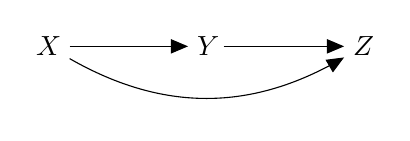
\begin{tikzpicture}[node distance=2cm, auto,>=triangle 45]
  \node (X) {$X$};
  \node [right of=X] (Y) {$Y$};
  \node [right of=Y] (Z) {$Z$};
  \draw[->] (X) --  (Y);
  \draw[->] (Y) -- (Z);
  \draw[->] (X) to [bend right=30] (Z);
\end{tikzpicture}
\caption{A coherent FFL.}
\end{figure}
%
\begin{python}
def coh_ffl_and(xs, yalpha=0.1, ybeta=0.1, kxy=0.5, zalpha=0.1, zbeta=0.1, kxz=0.5, kyz=0.5):
    ynow = 0
    ys = []
    znow = 0
    zs = []
    for x in xs:
        yb = 0
        if x > kxy:
            yb = ybeta
        ynew = update(ynow, yalpha, yb)
        ys.append(ynew)

        zb = 0
        if (x > kxz) and (ynow > kyz):
            zb = zbeta
        znew = update(znow, zalpha, zb)
        zs.append(znew)

        ynow = ynew
        znow = znew
    return ys, zs
\end{python}
%
And we'll test our function with the following code:
%
\begin{python}
xs = pulse(10,15,120) + pulse(40,100,120)
ys, zs = coh_ffl_and(xs, kyz=0.5)

p1, = plot(xs)
p2, = plot(ys)
p3, = plot(zs)
legend([p1,p2,p3,p4],["$X$","$Y$","$Z$"])
xlabel("time")
ylim(0,2)
\end{python}
%
In the example above, our $X$ signal represents two pulses -- a short pulse starting at time point 10, and a more sustained pulse at time point 40. As suggested by Shen-Orr et al., and illustrated in Fig.~\ref{fig:cohffland}, the coherent FFL motif with AND logic can act as a type of sign-sensitive filter.  $Z$ doesn't turn on until $Y$ reaches a critical threshold, but both $Y$ and $Z$ turn off simultaneously.
%
\begin{figure}[!ht]
    \centering
    \includegraphics[width=0.33\columnwidth]{./figures/hands-on12/fig-cohffland.png}
    \caption{Behavior of a coherent FFL with AND logic at $Z$.}\label{fig:cohffland}
\end{figure}


Now let's add some random noise to our input signal, $X$.
%
\begin{python}
nxs = xs + np.random.rayleigh(0.5,size=len(xs)) # add some random noise to the signal
nxs = abs(nxs - 0.5)
plot(nxs);
\end{python}
%
Let's see how the noise effects the network:
%
\begin{python}
ys, zs = coh_ffl_and(nxs, kyz=0.5)

p1, = plot(nxs)
p2, = plot(ys)
p3, = plot(zs)
legend([p1,p2,p3,p4],["$X$","$Y$","$Z$"])
xlabel("time")
ylim(0,2)
\end{python}
%
As shown in Fig.~\ref{fig:noisyffl}, $Z$ is effectively buffered from the noise.
%
\begin{figure}[!ht]
    \centering
    \includegraphics[width=0.33\columnwidth]{./figures/hands-on12/fig-noisyffl.png}
    \caption{Behavior of a coherent FFL with AND logic at $Z$, in response to a noisy input signal $X$.}\label{fig:noisyffl}
\end{figure}

\medskip
\begin{assignment}
Write an Python function that generates a coherent FFL with OR logic at $Z$ (i.e. $Z$ is on if either $X$ or $Y$ are above their respective thresholds), and illustrate this network motif for a variety of parameter settings.  How does the behavior of the coherent FFL with OR logic differ from the similar topology with AND logic?
\end{assignment}


\subsection{Incoherent FFLs}

Now we'll examine the behavior of an incoherent FFL, as illustrated in the figure below. As before, $X$ is an activator of both $Y$ and $Z$, but now $Y$ represses $Z$.

\begin{figure}[!ht]
\centering
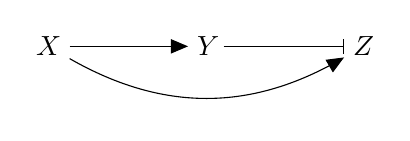
\begin{tikzpicture}[node distance=2cm, auto,>=triangle 45]
  \node (X) {$X$};
  \node [right of=X] (Y) {$Y$};
  \node [right of=Y] (Z) {$Z$};
  \draw[->] (X) --  (Y);
  \draw[-|] (Y) -- (Z);
  \draw[->] (X) to [bend right=30] (Z);
\end{tikzpicture}
\caption{An incoherent FFL.}
\end{figure}

\begin{python}
def incoh_ffl_and(xs, yalpha=0.1, ybeta=0.1, kxy=0.5, zalpha=0.1, zbeta=0.1, kxz=0.5, kyz=0.5):
    ynow = 0
    ys = []
    znow = 0
    zs = []
    for x in xs:
        yb = 0
        if x > kxy:
            yb = ybeta
        ynew = update(ynow, yalpha, yb)
        ys.append(ynew)

        zb = 0
        if (x > kxz) and (ynow < kyz):
            zb = zbeta
        znew = update(znow, zalpha, zb)
        zs.append(znew)

        ynow = ynew
        znow = znew
    return ys, zs
\end{python}
%
And we'll test our new function as follows:
%
\begin{python}
xs = pulse(10,40,180) + pulse(70,140,180)
ys, zs = incoh_ffl_and(xs, kyz=0.75)

p1, = plot(xs)
p2, = plot(ys)
p3, = plot(zs)

legend([p1,p2,p3,p4],["$X$","$Y$","$Z$"])
xlabel("time")
ylim(0,2)
\end{python}
%
This produces Fig.~\ref{fig:incohfll}.  Incoherent FFLs are capable of producing pulsatile behaviors. Notice how the length of the pulses in $Z$ are insensitive to longer input signals $X$ (they are however sensitive to very short pulses in $X$).
%
\begin{figure}[!ht]
    \centering
    \includegraphics[width=0.33\columnwidth]{./figures/hands-on12/fig-incohffl.png}
    \caption{Behavior of an incoherent FFL with AND logic at $Z$.}\label{fig:incohfll}
\end{figure}

\section{Repressilator}

Elowitz and Liebler (Nature, 403(6767):335-8) proposed that a synthetic network motif that they called the `repressilator' could generate sustained oscillatory behavior. This network motif consists of three genes that mutually repressor each other, as illustrated in Fig.~\ref{fig:repressilator}.
\begin{figure}[!ht]
\centering
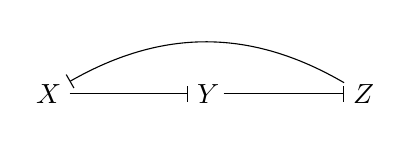
\begin{tikzpicture}[node distance=2cm, auto,>=triangle 45]
  \node (X) {$X$};
  \node [right of=X] (Y) {$Y$};
  \node [right of=Y] (Z) {$Z$};
  \draw[-|] (X) --  (Y);
  \draw[-|] (Y) -- (Z);
  \draw[-|] (Z) to [bend right=30] (X);
\end{tikzpicture}
\caption{The repressilator network motif.}\label{fig:repressilator}
\end{figure}
%
Let's implement the repressilator motif as a Python function:
\begin{python}
def repressilator(xalpha, xbeta, yalpha, ybeta, zalpha, zbeta, kxy=0.5, kyz=0.5, kzx=0.5, xinit=1, yinit=1, zinit=1, nticks=500):
    xnow = xinit
    xs = []
    ynow = yinit
    ys = []
    znow = zinit
    zs = []

    for i in range(nticks):
        if xnow < kxy:
            ya, yb = yalpha, ybeta
        else:
            ya, yb = yalpha, 0
        ynew = update(ynow, ya, yb)
        ys.append(ynew)

        if ynow < kyz:
            za, zb = zalpha, zbeta
        else:
            za, zb = zalpha, 0
        znew = update(znow, za, zb)
        zs.append(znew)

        if znow < kzx:
            xa, xb = xalpha, xbeta
        else:
            xa, xb = xalpha, 0
        xnew = update(xnow, xa, xb)
        xs.append(xnew)

        ynow = ynew
        znow = znew
        xnow = xnew

    return xs, ys, zs
\end{python}
%
And we can test it as we've done previously:
\begin{python}
xs,ys,zs = repressilator(0.1,1, 0.1,2, 0.1,2)
p1, = plot(xs)
p2, = plot(ys)
p3, = plot(zs)

legend([p1,p2,p3,],["$X$","$Y$","$Z$"])
xlabel("time")
\end{python}
%
\begin{figure}[!ht]
    \centering
    \includegraphics[width=0.33\columnwidth]{./figures/hands-on12/fig-repressilator.png}
    \caption{Behavior of the repressilator network motif.}\label{fig:repressdynamics}
\end{figure}



\medskip
\begin{assignment}
Spend some time exploring the parameter space of the repressilator motif.  Under what conditions does the system \emph{NOT} oscillate?  What parameters can you change to get longer oscillations (i.e. longer intervals between peak values for a given gene)?  Generate graphs to illustrate the cases above.
\end{assignment}

% \chapter{Building a Bioinformatics Pipeline}
% 
\section{Overview}

Many types of analyses, especially those involving genomic data, require the investigator to carry out a large number of sequential steps. For example, given a set of uncharacterized genes in your organism of interest you might want to find out as much as you can about the structure and function of the proteins they encode, search for related proteins in other organisms, and try to identify pathways that they might be involved in. If you had only a single gene of interest you might apply each of the appropriate software tools by hand to carry out such an analysis. However, when the number of genes of interest grows beyond a small number (say 10-15) doing such an analysis by hand starts to become tedious and error prone.  A bioinformatics pipeline can help to automate this process, will make the analysis easier to replicate or apply to new sets of genes, and can be modified to include additional tasks.  Writing out a series of analysis steps as a pipeline also helps us to achieve the goal of `reproducible research' in the same way that knitr helps you to do so in R.

We're going to build an example bioinformtics pipeline using BioPython along with several command line programs.  This pipeline will incorporate such features as web based queries and conversion of information between different file formats.

\section{The Pipeline}


The tasks carried out by the pipeline will be as follows:

\begin{itemize}

\item Read in a nucleotide sequence from a FASTA file
\item Translate the nucleotide sequence to an amino acid sequence
\item Do a blastp search against human and fly proteins in the Swiss-Prot database using an interface to the NCBI web version of BLAST
\item Download protein sequences for the best blast hits from Swiss-Prot
\item Use MAFFT to do a multiple alignment of the original amino acid sequence and the presumed orthologs generated via the blast search
\item Analyze the query protein for known protein domains using HMMER and Pfam
%\item Use a web service to query the KEGG pathways database to look for pathways that include orthologues to your gene of interest

\end{itemize}


You will need a working installation of Python (2.7+), IPython, and the BioPython library (1.59+) as well as the command line tools we installed last week (MAFFT, HMMER).

\section{MAFFT}

MAFFT is a multiple sequence alignment program. It's relatively fast and a number of studies have shown that it is amongst the best performing multiple sequence aligners. MAFFT is usually the sequence aligner I reach for first.  Clustalw is the `classic' alignment tool, so it's useful to have on your system, but MAFFT usually gives better alignments (though Clustalw2 is supposed to address some of the short-comings of the older versions of Clustalw). See the \href{http://mafft.cbrc.jp/alignment/software/}{MAFFT website} for additional references and information.

There are pre-compiled MAFFT binaries available on the MAFFT website.

Once you've installed MAFFT check the installation location and confirm that the binary is working (on Windows, add the MAFFT install directory to your PATH):
%
\begin{code}
$ which mafft
/usr/local/bin/mafft
$ mafft  # type ctrl-c to exit from the interactive prompt

---------------------------------------------------

   MAFFT v6.864b (2011/11/10)

        Copyright (c) 2011 Kazutaka Katoh
        NAR 30:3059-3066, NAR 33:511-518
        http://mafft.cbrc.jp/alignment/software/
---------------------------------------------------
\end{code}

\subsection{Testing MAFFT}

Once you've confirmed that MAFFT is properly installed, let's test it with some real data. Download the |fungal-ras.fas| file from the class website. This file includes protein sequences of Ras-family proteins from a number of different fungi.  Ras proteins are small GTPases that are involved in cellular signal transduction.  Ras signaling is often involved in cellular growth and differentiation and mutations that affect Ras signaling often lead to cancer.  We'll use this data to do some quick tests to confirm that our software tools are working correctly. Of course, when putting together an analysis pipeline for your own purposes you'll want to spend a fair amount of time reading the documentation (and related papers) for each tool and make sure you understand the various options and settings.

Let's run Clustalw and MAFFT to align the Ras sequences:
%
\begin{bash}
$ mafft --auto fungal-ras.fas > fungal-ras-mafft.fas
\end{bash}
%
The commands above should produce the following file: |fungal-ras-mafft.fas| (MAFFT).  To visualize the alignments there are a variety of different multiple alignment viewers. One such program is \href{http://www.jalview.org/}{Jalview}, a free cross platform, multiple alignment viewer/editor written in Java.  Take a look at the MAFFT alignment using Jalview.


\section{HMMER}

HMMER is an implementation of a profile Hidden Markov Model (HMM) for protein sequence analysis. You can read up on HMMER at the \href{http://hmmer.janelia.org/}{HMMER website}. We will use it here for finding protein domains in sequences in conjuction with the PFAM database.


\subsection{Get the PFAM HMM library}

We will be using the Pfam database (Release 26) in conjunction with HMMER to search for known protein domains in our sequences of interest. Since the the Pfam HMM libraries are large I'll try and provide a couple of thumb drives with the necessary library. If you're using this document outside of class you can download the necessay library as follows:
%
\begin{code}
$ curl -O ftp://ftp.sanger.ac.uk/pub/databases/Pfam/releases/Pfam26.0/Pfam-A.hmm.gz
\end{code}
%
This is a large file (202MB) and decompresses to an even larger file (approx. 1GB). Make sure you have adequate disk space. On OS X or Windows using Cygwin you can unzip it as follows:
%
\begin{code}
$ gunzip Pfam-A.hmm.gz
\end{code}
%
If you aren't using Cygwin on Windows you can download the open source program \href{http://www.7-zip.org/}{7-zip} which can unzip gzip'd files (and many other common compression formats).

\subsection{Testing HMMER}

To test out HMMER and Pfam download the |Rme1.fas| file from the class wiki. Rme1 is a transcription factor that regulates sporulation and meiosis in budding yeast, \textit{Saccharomyces cerevisiae}.  We'll use HMMER to analyze the domain structure of Rme1.

The first thing you'll need to do is run |Pfam-A.hmm| through the |hmmpress| program which prepares the HMM database for fast scanning by creating binary files. This might take a few minutes depending on the speed of your machine.

\begin{code}
$ hmmpress Pfam-A.hmm
\end{code}

This will create a number of additional files in the same directory as |Pfam-A.hmm|. We can now use |hmmscan| to search for known protein domains included in the Pfam database.

\begin{code}
$ hmmscan Pfam-A.hmm Rme1.fas > Rme1-Pfam-out.txt
\end{code}

The default output from |hmmscan| is designed to be human readable. Open |Rme1-Pfam-out.txt| in a text editor to see the output. For outputs that are easier to parse computationally use the |--tblout| or |--domtblout| options to save output in a tabular format.

\begin{code}
$ hmmscan --domtblout Rme1-output.txt -o /dev/null Pfam-A.hmm Rme1.fas
\end{code}

This call produces a file |Rme1-output.txt| that contains a space delimited text file summarizing the per-domain output. The |-o| option redirects the main human-readable output (in this case to the `bit-bucket', /dev/null). You can then manipulate the tabular output in |Rme1-output.txt| using standard Unix tools like |awk|.

See pp.\,24-26  of the \href{ftp://selab.janelia.org/pub/software/hmmer3/3.0/Userguide.pdf}{HMMER user guide} for more info on the |hmmscan| program and settings. E-values and bit-scores are the criteria you want to look at when trying to judge which domains you sequence of interest has good matches to.  HMMER bit scores reflect the extent to which a sequence is a good match to a  profile model (higher bit scores are better matches). See p.\,43 of the HMMER 2.3 user guide (use Google to find a copy of the older version of the HMMER manual) for a discussion of E-values and bit scores.  If you examine the output file |Rme1-output.txt| you'll see that the model with the lowest E-values and highest bit-scores is a ``zinc finger'' domain.  There are three such domains in the Rme1 protein (see the column labeled ``N'' in the output), though two of them are weaker matches (larger E-values). Rme1 is a zinc finger transcriptional factor. The two weaker zinc finger domains are weak matches to the HMM model for zinc fingers but are nonetheless functional domains.


\section{Biopython}

Now we turn our attention to Biopython.  As we build our pipeline I will first demonstrate the use of various modules, classes, and functions in the interactive shell and then I will give a set of functions that consolidate the commands to make them convenient to use.

\subsection{Test files}

Download the file |unknown1.fas| and |unknown2.fas| from the class website. I recommend you place these in |~/tmp|.

\subsection{Reading in a single sequence from a FASTA file}

Fire up and ipython interpreter, either a text based command line (|ipython --pylab|) or an ipython notebook (|ipython notebook --pylab=inline|).


We'll start by showing how to read sequence data out of a FASTA file:
\begin{python}
>>> cd ~/tmp
>>> from Bio import SeqIO
>>> u1 = SeqIO.read('unknown1.fas','fasta')
>>> type(u1)
<class 'Bio.SeqRecord.SeqRecord'>
>>> u1
SeqRecord(seq=Seq('ATGATGAATTTTTTTACATCAAAATCGTCGAAT
CAGGATACTGGATTTAGCTCT...TGA', SingleLetterAlphabet()),
id='YHR205W', name='YHR205W', description='YHR205W  Chr 8', dbxrefs=[])
>>> u1.name
'YHR205W'
>>> u1.description
'YHR205W  Chr 8'
>>> u1.seq
Seq('ATGATGAATTTTTTTACATCAAAATCGTCGAATCAGGATACTGG
ATTTAGCTCT...TGA', SingleLetterAlphabet())
>>> u1.seq[:10]
Seq('ATGATGAATT', SingleLetterAlphabet())
>>> u1.seq[0]
'A'
>>> u1.seq[9]
'T'
>>> u1.seq[:10].tostring()
'ATGATGAATT'
>>> u1.seq.translate()[:10]
Seq('MMNFFTSKSS', HasStopCodon(ExtendedIUPACProtein(), '*'))
\end{python}

|SeqIO| is a sub-module of the top-level module Biopython module |Bio|.  |SeqIO.read| reads a single sequence object from a file and returns an instance of a |SeqRecord| class (defined in the Biopython package). A \emph{class} is a programming concept that groups data and functions that operate on that data into a single object. For example, in the code above we used the |.name| and |.description| attributes to examine information about the sequence (this information was retrieved from the FASTA file itself).  A |SeqRecord| holds a |Seq| object (yet another class!) as well as accessory information like the name of the sequence, a description, etc. |Seq| objects act very much like strings in terms of slicing and element access but they also have specialized function like |.translate()| that can be used to translate a nucleotide sequence into a peptide sequence.

\subsubsection{Reading in multiple sequences from a FASTA file}

In the code above we demonstrated how to read a single sequence from a FASTA file.  Here we demonstrate how to read multiple sequences.  The key difference is the use of the |SeqIO.parse()| function rather than |SeqIO.read()|.

\begin{python}
>>> u2 = SeqIO.parse('unknown2.fas', 'fasta')
>>> type(u2)
<type 'generator'>
>>> s1 = u2.next()
>>> type(s1)
<class 'Bio.SeqRecord.SeqRecord'>
>>> s1
SeqRecord(seq=Seq('ATGTCATCAAAACCTGATACTGGTTCGGA
AATTTCTGGCCCTCAGCGACAGGAA...TGA', SingleLetterAlphabet()),
id='YJL005W', name='YJL005W', description='YJL005W', dbxrefs=[])
>>> s1.seq
Seq('ATGTCATCAAAACCTGATACTGGTTCGGAAATTTCTGGCC
CTCAGCGACAGGAA...TGA', SingleLetterAlphabet())
>>> s2 = u2.next()
>>> s2
SeqRecord(seq=Seq('ATGTCATCAAATCATGCTATTAGTCCAGAA
ACTTCTGGCTCTCATGAGCAACAA...TGA', SingleLetterAlphabet()),
id='MIT_Sbay_c342_13338', name='MIT_Sbay_c342_13338',
description='MIT_Sbay_c342_13338', dbxrefs=[])
>>> s3 = u2.next()
>>> s4 = u2.next()
>>> s5 = u2.next()
---------------------------------------------------------------------------
StopIteration                             Traceback (most recent call last)
/Users/pmagwene/Desktop/tmp/<ipython console> in <module>()
StopIteration:
\end{python}

In this case the |SeqIO.parse| function returns an object that has \emph{iterator} semantics (technically it's a `generator' but this is a technical difference that you can ignore for now). An iterator is an object that `acts like' a sequence (e.g. a list or tuple), but there are some major differences. The most important one is that an iterator does not have to compute the entire sequence at once. In the case of the |SeqIO.parse()| function that means that if you have a FASTA file with thousands of sequence entries it wouldn't try to suck them all into memory. The |.next()| method is used to call successive sequence entries in the FASTA file. When you call |.next()| on the iterator(generator) instance you get back |SeqRecords|, one at a time. However, as the lost call demonstrates if there is no 'next' item in the iterator it raises a |StopIteration| exception. For more info about iterators and generators see Norman Matloff's  \href{https://github.com/pmagwene/Bio313/raw/master/lecture-13/PyIterGen.pdf}{Tutorial on Python Iterators and Generators}.

The steps for reading a FASTA sequence file can be wrapped up in the following function. We'll place each of the functions we develop in a module called |pipeline.py| (place this in your working directory or your |PYTHONPATH|).  As you progress through the pipeline design you will add additional functions to this module.

\begin{python}
# pipeline.py -- a simple bioinformatics pipeline
from Bio import SeqIO

def read_fasta(infile):
    """Read a single sequence from a FASTA file"""
    rec = SeqIO.read(infile,'fasta')
    return rec

def parse_fasta(infile):
    """Read multiple sequences from a FASTA file"""
    recs = SeqIO.parse(infile,'fasta')
    return [i for i in recs]
\end{python}

\subsubsection{List comprehensions}
The |parse_fasta()| function  above introduces another new concept called \emph{list comprehensions}. A list comprehension is a compact way of applying a function to each element in a sequence. In this case the list comprehension implicitly called |.next()| to get all the |SeqRecords| from the generator returned by |SeqIO.parse()|.  You'll recall that most functions in R works in a vector-wise manner. List comprehensions provide similar semantics for Python.  Below are some simpler examples of list comprehensions. Try and predict the output of each of these before typing them in:

\begin{python}
In [1]: x = [2,4,6,8,10]
In [2]: [i**2 for i in x]
Out[2]: ???
In [3]: y = ['bob', 'tab', 'rob', 'snob']
In [4]: def juvenilize(s):
   ...:     return str(s) + "by"
   ...:
In [5]: [juvenilize(i) for i in y]
Out[5]: ???
\end{python}

You can  use the |read_fast()| function as follows:
\begin{python}
>>> import pipeline
>>> recs = pipeline.parse_fasta('unknown2.fas')
>>> len(recs)
4
>>> [i.name for i in recs]
['YJL005W', 'MIT_Sbay_c342_13338', 'MIT_Smik_c333_12160', 'MIT_Spar_c300_12282']
\end{python}

Note that the |parse_fasta()| function will return a list of |SeqRecords| even when there is only a single sequence in the file. In contrast, if you use the function |read_fasta()| on a FASTA file with more than one sequence it will raise an error.

\subsection{Translating nucleotide sequence to a protein sequence}

The next step is to translate each  DNA sequence into a corresponding protein sequence. This is very easy using the |.translate()| method associated with the |Seq| class.

\begin{python}
>>> recs[0].seq.translate()
Seq('MSSKPDTGSEISGPQRQEEQEQQIEQSSPTEANDRSIHDEV
PKVKKRHEQNSGH...ST*', HasStopCodon(ExtendedIUPACProtein(), '*'))
\end{python}
%
Note that the above code returns an object of type |Seq|. That's usually what we want if we're manipulating nucleotide or protein sequences but if we want to write our translated sequences back out into a file we need to create new |SeqRecords|. I illustrate this in the function below (add this to |pipeline.py|).

\begin{python}
from Bio import Seq
from Bio import SeqRecord

def translate_recs(seqrecs):
    """ nucleotide SeqRecords -> translated protein SeqRecords """
    proteins = []
    for rec in seqrecs:
        aaseq = rec.seq.translate()
        protrec = SeqRecord.SeqRecord(aaseq, id=rec.id, name=rec.name,
        			      description=rec.description)
        proteins.append(protrec)
    return proteins
\end{python}

We can then encapsulate the whole process of converting a nucleotide FASTA file to a peptide sequence FASTA file as so (add these to |pipeline.py|):

\begin{python}
def write_fasta(recs, outfile):
    ofile = open(outfile, 'w')
    SeqIO.write(recs, ofile, 'fasta')

def translate_fasta(infile, outfile):
    """ nucleotide fasta file -> protein fasta file """
    nrecs = parse_fasta(infile)
    precs = translate_recs(nrecs)
    write_fasta(precs, outfile)
\end{python}

|open()| is a built-in Python function that when called with the |'w'| argument opens a file for writing. When called with |'r'| as it's second argument it opens a file for reading.

We can use our |translate_fasta| function from the Python interpreter like so:

\begin{python}
>>> reload(pipeline)
<module 'pipeline' from '/Users/pmagwene/synchronized/pyth/pipeline.py'>
>>> pipeline.translate_fasta('unknown2.fas', 'unknown2-protein.fasta')
\end{python}
%
Take a moment to open the file \texttt{unknown2-protein.fasta} in a text editor to confirm that the file now hold amino acid sequences rather than nucleotide sequences.

\subsubsection{Globbing to get multiple files of a given type}
As an aside, what if we wanted to repeat this for a whole directory full of DNA sequences in separate FASTA files?  Here's a function to help accomplish that task:
\begin{python}
import glob

def inout_pairs(insuffix, outsuffix):
    """ Files in directory with given suffix -> list of tuples w/ (infile,outfile)"""
    infiles = glob.glob('*'+insuffix)
    pairs = []
    for infile in infiles:
        inprefix = infile[:-len(insuffix)]
        outfile = inprefix + outsuffix
        pairs.append((infile,outfile))
    return pairs
\end{python}
%
The |glob| module gives you filename `globbing' functionality. Globbing is a means of matching specified file or pathnames; you can think about this as a simplified class of regular expressions.  For example, you're probably familiar with command line searches like:
\begin{python}
$ ls *.fas   # list all files with the extension .fas
$ ls unk*   # list all files that begin with 'unk'
\end{python}
%
The |inout_pairs()| function we defined above allows us to glob file files with the given |insuffix| and create a corresponding set of names for output files. The following illustrates this:

\begin{python}
>>> pairs = pipeline.inout_pairs('.fas', '-protein.fasta')
>>> pairs
[('unknown1.fas', 'unknown1-protein.fasta'),
('unknown2.fas', 'unknown2-protein.fasta')]
>>> from Bio.Data.CodonTable import TranslationError
>>> for (i,o) in pairs:
...     try:
...         pipeline.translate_fasta(i,o)
...     except TranslationError:
...         continue
...
...
>>> ls *.fas*  # only works in ipython
unknown1-protein.fasta  unknown1.fas  unknown2-protein.fasta  unknown2.fas
\end{python}
%
Note that I changed the file suffix from |.fas| to |.fasta| on the output files. This isn't necessary but I find that doing so makes it easy to sort through large directories to distinguish generated files from the original files. The |inout_pairs()| function will come in handy when we combine our functions to generate a multi-sequence pipeline.

Another new concept I introduced in the for loop above is |try-except| block for exception handling.  The Python starts by executing the code in the |try| clause.  If there are no problems the |except| clause is ignored.  However, if an exception (error) is raised than it evaluates the |except| clause. In this case, our |except| clause says if the error is an exception of type |TranslationError| (defined in |Bio.Data.CodonTable|) then ignore it and just keep working.  However, any other exception will stop program execution, as we haven't included any general error handling code. See Downey, Chap 14 for more discussion of exception handling.


\subsection{BLAST searches via the NCBI server}

We can use Biopython do network based BLAST searches. Here we will use blastp to search against protein sequences in the Swiss-Prot database.

\begin{python}
>>> from Bio.Blast import NCBIWWW, NCBIXML
>>> prot1 = pipeline.read_fasta('unknown1-protein.fasta')
>>> results_handle = NCBIWWW.qblast('blastp','swissprot',prot1.seq.tostring(), entrez_query='(Homo sapiens[ORGN])')
>>> results = results_handle.read()
>>> sfile = open('prot1_blast.out','w')
>>> sfile.write(results)
>>> sfile.close()
>>> blast_out = open('prot1_blast.out','r')
>>> brec = NCBIXML.read(blast_out)
>>> brec
<Bio.Blast.Record.Blast instance at 0x2ec22d8>
>>> len(brec.alignments) # we got 50 blast hits in the query
50
>>> brec.alignments[0]
<Bio.Blast.Record.Alignment instance at 0x2ec23a0>
>>> brec.alignments[0].accession
u'P31749'
\end{python}

This code introduces another concept we'll call the \emph{Producer-Consumer} pattern. The Producer-Consumer pattern is a general programming concept, but the key here is that the pattern generalizes the problem of parsing complex biological data types. The producer does the work of getting the information from a file (or from the web in this case). The consumer process the information into a form we can use. In the code above the function |NCBIWWW.qblast()| is the producer and |NCBIXML.read()| plays the role of the consumer. This pattern is used over and over again in Biopython so you should spend some time trying to understand the general idea. See the Biopython tutorial for a more complete discussion.

Our BLAST query returned the information in the form of XML data.  XML stands for `Extensible Markup Language', and is a generic way to encode documents in machine-readable form.  XML data is usually plain text -- go ahead and open up the file |prot1_blast.out| in a text editor to see the output. Since XML is a generic format, specific types of XML documents need a `schema' or `grammar' that specifies how the document is to be read and interpretted. In the example above, the module |NCBIXML| knows how to handle XML data returned from NCBI, hence our use of the function |NCBIXML.read()|.

In the example given, we limited our query to sequences from humans. If we wanted to include all metazoan sequences we could pass |'(Metazoa[ORGN])'| as the argument to |entrez_query|. If we didn't want to limit our search at all we would simply not include that argument (i.e. accept the default). The BLAST output is fairly complicated. See the BioPython tutorial section 7.5 for a complete breakdown of all the fields in the BLAST output.

Again, the commands above are rather involved so let's wrap them up in a function:

\begin{python}
from Bio.Blast import NCBIWWW, NCBIXML

def blastp(seqrec, outfile, database='nr', entrez_query='(none)'):
    handle = NCBIWWW.qblast('blastp', database, seqrec.seq.tostring(),
    				entrez_query=entrez_query)
    results = handle.read()
    sfile = open(outfile, 'w')
    sfile.write(results)
    sfile.close()
    bout = open(outfile, 'r')
    brecord = NCBIXML.read(bout)
    return brecord

def summarize_blastoutput(brecord):
    hits = []
    for alignment in brecord.alignments:
        expect = alignment.hsps[0].expect
        accession = alignment.accession
        hits.append((expect,accession))
    hits.sort() # will sort tuples by their first value (i.e. expect)
    return hits
\end{python}

We can use this code as follows:
\begin{python}
>>> humanblast = pipeline.blastp(prot1, 'prot1-hum-blast.out', database='swissprot', entrez_query='(Homo sapiens[ORGN])')
>>> flyblast = pipeline.blastp(prot1, 'prot1-fly-blast.out', database='swissprot', entrez_query='(Drosophila melanogaster[ORGN])')
>>> humanhits = pipeline.summarize_blastoutput(humanblast)
>>> flyhits = pipeline.summarize_blastoutput(flyblast)
>>> humanhits[0] # the first number is the E-value for the BLAST search
(4.98013e-95, u'P31749')
>>> print humanhits[0][1]  # prints the swissprot accession number
P31749
>>> flyhits[0]
(4.09304e-96, u'Q8INB9')
\end{python}

Go to the UniProt \href{http://www.uniprot.org/}{website} and use the search box to lookup those accession numbers.



\subsection{Getting records from Swiss-Prot}

For a small number of accession numbers it's easy to use the web interface to UniProt (Swiss-Prot). For hundred of blast hits that's just not an option. Conveniently, we can use Biopython to query the Swiss-Prot database to retrieve information about these presumed orthologs. You can access the Swiss-Prot database as follows:

\begin{python}
>>> from Bio import ExPASy
>>> from Bio import SwissProt
>>> handle1 = ExPASy.get_sprot_raw(humanhits[0][1]) # access with the accession number
>>> rec1 = SwissProt.read(handle1)
>>> print rec1.description
RecName: Full=RAC-alpha serine/threonine-protein kinase; EC=2.7.11.1; AltName:
Full=RAC-PK-alpha; AltName: Full=Protein kinase B; Short=PKB; AltName: Full=C-
AKT;
>>> rec1.comments[0]
"FUNCTION: AKT1 is one of 3 closely related serine/threonine- protein kinases (AKT1, AKT2 and AKT3) called the AKT kinase, and which regulate many processes including metabolism, proliferation, cell survival, growth and angiogenesis.
... output truncated ..."
>>> print dir(rec1) # lets see what other attributes the record has
['__doc__', '__init__', '__module__', 'accessions', 'annotation_update', 'comments', 'created', 'cross_references', 'data_class', 'description', 'entry_name', 'features', 'gene_name', 'host_organism', 'host_taxonomy_id', 'keywords', 'molecule_type', 'organelle', 'organism', 'organism_classification', 'references', 'seqinfo', 'sequence', 'sequence_length', 'sequence_update', 'taxonomy_id']
>>> print rec1.gene_name
Name=AKT1; Synonyms=PKB, RAC;
>>> print rec1.sequence[:25] # first 25 amino acids
MSDVAIVKEGWLHKRGEYIKTWRPR
\end{python}

Here's some functions to make this more convenient:

\begin{python}
from Bio import ExPASy
from Bio import SwissProt

def get_swissrec(accession):
    handle = ExPASy.get_sprot_raw(accession)
    record = SwissProt.read(handle)
    return record

def swissrec2seqrec(record):
    seq = Seq.Seq(record.sequence, Seq.IUPAC.protein)
    s = SeqRecord.SeqRecord(seq, description=record.description,
                id=record.accessions[0], name=record.entry_name)
    return s
\end{python}
%
And here is an example of how we can apply these functions:

\begin{python}
>>> ids = [humanhits[0][1], flyhits[0][1]]
>>> ids
[u'P31749', u'Q8INB9']
>>> swissrecs = [pipeline.get_swissrec(i) for i in ids]
>>> seqs = [pipeline.swissrec2seqrec(i) for i in swissrecs]
>>> seqs[0]
SeqRecord(seq=Seq('MSDVAIVKEGWLHKRGEYIKTWRPRYFLLKNDGTFIGYKERPQDVDQREAPLNN...GTA', IUPACProtein()), id='P31749', name='AKT1_HUMAN', description='RecName: Full=RAC-alpha serine/threonine-protein kinase; EC=2.7.11.1; AltName: Full=Protein kinase B; Short=PKB; AltName: Full=Protein kinase B alpha; Short=PKB alpha; AltName: Full=Proto-oncogene c-Akt; AltName: Full=RAC-PK-alpha;', dbxrefs=[])
>>> seqs[1]
SeqRecord(seq=Seq('MNYLPFVLQRRSTVVASAPAPGSASRIPESPTTTGSNIINIIYSQSTHPNSSPT...SMQ', IUPACProtein()), id='Q8INB9', name='AKT1_DROME', description='RecName: Full=RAC serine/threonine-protein kinase; Short=DAkt; Short=DRAC-PK; Short=Dakt1; EC=2.7.11.1; AltName: Full=Akt; AltName: Full=Protein kinase B; Short=PKB;', dbxrefs=[])
>>> seqs.append(prot1)  # add our original protein sequence to the list
>>> pipeline.write_fasta(seqs, 'unknown1-plus-human-fly.fasta')
\end{python}


\subsection{Multiple sequence alignment via MAFFT}

We've now generated a new FASTA file that includes our original protein sequence and the sequences for the human and fly BLAST best hits.  We will use MAFFT to perform a multiple alignment. Biopython has built in code to simplify command line usage of common alignment programs like CLUSTALW, MAFFT, and MUSCLE.  However I'll show you how to do this with your own code using the |subprocess| module.  Knowing how the |subprocess| module works is useful because it allows you to interface with any command line program from within Python.

The |subprocess| module allows your Python code to start other programs (child processes) and send/get input and output from those same processes. When we use the subprocess module we're putting the Unix design element of `Everything is a file or process' to use. Here's a simple example:

\begin{python}
>>> import subprocess
>>> subprocess.call(["ls","-l"])
# on windows the equivalent command is
# subprocess.call(["dir",],shell=True)
# output is NOT shown in ipython notebook, instead
# a return code (0 if the command worked) is shown
total 11696
-rw-r--r--   1 pmagwene  staff    93514 Nov 22 19:36 prot1-fly-blast.out
-rw-r--r--   1 pmagwene  staff   109635 Nov 22 19:35 prot1-hum-blast.out
-rw-r--r--   1 pmagwene  staff   109635 Nov 22 19:19 prot1_blast.out
-rw-r--r--   1 pmagwene  staff     2308 Nov 22 20:07 unknown1-plus-human-fly.fasta
-rw-r--r--   1 pmagwene  staff      854 Nov 22 16:46 unknown1-protein.fasta
-rwx------   1 pmagwene  staff     2535 Nov 22 15:38 unknown1.fas
-rw-r--r--@  1 pmagwene  staff    24849 Nov 22 16:25 unknown2.fas
-rw-r--r--   1 pmagwene  staff     8331 Nov 22 16:46 unknowns-protein.fasta
\end{python}

The above code uses a convenience function |call()| in the |subprocess| module. We'll use the same function to run MAFFT:

\begin{python}
import subprocess

def mafft_align(infile, outfile):
    ofile = open(outfile,'w')
    retcode = subprocess.call(["mafft",infile], stdout=ofile)
    ofile.close()
    if retcode != 0:
        raise Exception("Possible error in MAFFT alignment")
\end{python}

And we put it to use as follows:
\begin{python}
In [8]: reload(pipeline)
In [8]: pipeline.mafft_align('unknown1-plus-human-fly.fasta', 'unknown1-alignment.fasta')
\end{python}

If all went well this should have created the file |unknown1-alignment.fasta| in your directory.  Open this alignment using JalView to examine the alignment in more detail.

\subsection{Searching for protein domains using HMMER and Pfam}

As the final step of our pipeline we'll use HMMER and the Pfam database to search for known protein domains in our original protein. This assumes you have the HMMER binaries and Pfam database installed as demonstrated in last weeks exercises and that you've already run |hmmpress| against the Pfam database. Again we write a small wrapper function using the |subprocess| module. This time we'll use the |Popen| class to illustrate how we can capture the output produced by |hmmpfam|. Note that if you haven't installed the HMMER binaries to one of the standard locations you might need to specify the full path to the |hmmscan| executable in the code below.

\begin{python}
def hmmer_pfam(infilename, outfilename, pfamdb):
    pipe = subprocess.Popen(["hmmscan", pfamdb, infilename],
            stdout=subprocess.PIPE).stdout
    output = pipe.read() # this gives us the output of our command
    outfile = open(outfilename, 'w')
    outfile.write(output)
    outfile.close()
\end{python}


This function can be called like this:

\begin{python}
# change the last argument to match the path to your Pfam database.
>>> pipeline.hmmer_pfam('unknown1-protein.fasta', 'unknown1-domains.out', '/Users/pmagwene/tmp/Pfam-A.hmm')
\end{python}

As before this search may take several minutes.


\subsection{Putting it all together}

We've generated a variety of functions that take care of the major steps of our pipeline. It's time to put the steps together to automate the entire process.

\begin{python}
def oneseq_pipeline(infilename, pfamdb=None,
                    compareto=['Homo sapiens','Drosophila melanogaster'],
                    skipHMMER = True,extension="XX"):
    # translate nucleotide sequence to protein seq
    protout = 'protein-' + infilename + extension
                # add the extension so all generated files have
                # different extension than input files

    translate_fasta(infilename, protout)

    # run blastp on protein sequence against swissprot and extract best hits
    protrec = parse_fasta(protout)[0]
    blastout ='blast-' + protout
    besthitids = []
    for organism in compareto:
        equery = '(%s[ORGN])' % organism # create the entrez organism query
        brecord = blastp(protrec, blastout, database='swissprot', entrez_query=equery)
        bhits = summarize_blastoutput(brecord)
        besthitids.append(bhits[0][1])

    # download corresponding records from Swiss-Prot
    swissrecs = [get_swissrec(i) for i in besthitids]
    seqs = [swissrec2seqrec(i) for i in swissrecs]
    seqs.append(protrec)

    # write FASTA file with best hits plus original protein sequence
    plusout = 'blasthits-' + protout + '.XML'
    write_fasta(seqs, plusout)

    # do multiple alignment via mafft
    mafft_align(plusout, 'aligned-' + protout)

    # search for domains via HMMER/Pfam
    if not skipHMMER:
        if pfamdb is not None:
            hmmerout = 'hmmer-' + protout
            hmmer_pfam(protout, hmmerout, pfamdb)

\end{python}

Our function can take as input a FASTA file with a single sequence or with multiple sequences. In the case of a multiple sequences it assumes that the `target' sequence for the search is the first sequence in the file. Also, note the |skipHMMER| argument included in the function. The HMMER search takes a relatively long time and doing it sequence by sequence is not very efficient so by default the pipeline will skip this step. If you want to include the HMMER step than specify the Pfam database file and set |skipHMMER=False|.

\subsubsection{Testing out the pipeline}
To test out the function we do:
\begin{python}
>>> reload(pipeline)
>>> pipeline.oneseq_pipeline('unknown1.fas')
\end{python}
%
This will create four new FASTA files:
\begin{enumerate}[1), noitemsep, topsep=0.5ex]
\item |protein-unknown1.fasXX|
\item |blast-protein-unknown1.fasXX.XML|
\item |blasthits-protein-unknown1.fasXX|
\item |aligned-protein-unknown1.fasXX|
\end{enumerate}
%
These respectively contain:
\begin{enumerate}[1), noitemsep,topsep=0.5ex]
\item the amino acid sequence translated from the nucleotide sequence given as input
\item the XML output of the qblast query to NCBI
\item the amino acid sequences for the BLAST hits returned from NCBI
\item the MAFFT multiple alignment of the protein sequences.
\end{enumerate}

\medskip
Let's now test the pipeline using an alternate set organisms:
\begin{python}
>>> pipeline.oneseq_pipeline('unknown1.fas', compareto=["Homo sapiens","Mus musculus","Caenorhabditis elegans"])
\end{python}

For completeness let's also test the pipeline with the HMMER step included:
\begin{python}
>>> pipeline.oneseq_pipeline('unknown1.fas', '/home/pmagwene/tmp/Pfam-A.hmm',
skipHMMER=False)
\end{python}

\subsubsection{Extending the pipeline to deal with multiple inputs}
Now that we're confident out single sequence pipeline function works it can be easily adapted to deal with multiple input files:

\begin{python}
def multiseq_pipeline(inext, pfamdb=None,
                compareto=['Homo sapiens','Drosophila melanogaster'],
                skipHMMER=True):
    inout = inout_pairs(inext, 'XX')
    infiles = [i[0] for i in inout]
    for filename in infiles:
        print "Processing %s" % filename
        oneseq_pipeline(filename, pfamdb, compareto, skipHMMER)
\end{python}

To test the complete multi-sequence pipeline delete all the generated files (so that only \verb=unknown1.fas= and \verb=unknown2.fas= are in the unknowns directory) and try the following:
\begin{python}
>>> pipeline.multiseq_pipeline('.fas')
\end{python}

Given our example data this function will process just two input files.  However, you can add an arbitrary number of additional `.fas' files to the directory and the pipeline will process those as well with exactly the same command.

There are a number of ways the pipeline could be sped up. One obvious improvement would be to utilize a local installation of BLAST and the respective databases. However, optimization is often a complex task. The pipeline we developed here doesn't require us to install BLAST (which can be somewhat involved) and provides adequate performance for a modest number of sequences. It is possible to turn this set of Python functions into a program that you could run from the command line (rather than the Python interpeter) just like any other Unix program.


\section{The pipeline.py module}
The pages that follow give the complete code listing for the |pipeline.py| module.

\newpage
\lstinputlisting[language=python]{./hands-on13/pipeline.py}


%\appendix
%\chapter{The Unix Command Line}
%\input{./supplements/unix-commandline.tex}


%
%
% \bibliography{../researchjournal-refs.bib}
% \bibliographystyle{cbe}

\end{document}

